%%%%%%%%%%%%%%%%%%%%%%%%%%%%%%%%%%%%%%%%%%%%%%%%%%%%%%
% Tesis Romano Trad                              %
%%%%%%%%%%%%%%%%%%%%%%%%%%%%%%%%%%%%%%%%%%%%%%%%%%%%%%
\documentclass[11pt,A4paper,oneside]{book}

% Set equal margins on book style
\setlength{\oddsidemargin}{43pt}
\setlength{\evensidemargin}{43pt}
\setlength{\marginparwidth}{47pt}
\setlength{\footskip}{10pt}



\usepackage[spanish]{babel} % para escribir en español
\usepackage[utf8x]{inputenc}% solución a los acentos
\usepackage{verbatim}       % para insertar código sin perder formato
\usepackage{amsmath}        % fórmulas matemáticas
\usepackage{graphicx}       % para insertar imágenes
\usepackage{longtable}
\usepackage{float}
\usepackage{subfig}
\usepackage{colortbl}
\usepackage{tabularx}
%\usepackage{algorithm}
%\usepackage{algorithmic}
\newcommand{\HRule}{\rule{\linewidth}{0.5mm}}
\begin{document}            % inicio del documento

%\title{Implementación HW/SW de Arquitecturas de Clasificacion de Paquetes en Logica Reconfigurable}
%\author{Luis Roberto Romano, \and Jairo Nicolas Trad}
%\institute{Universidad Nacional de Córdoba}
%\date{Universidad Nacional de Córdoba}
%\maketitle

\begin{titlepage}
\begin{center}

\includegraphics[width=0.4\textwidth]{Logo-UNC.eps}

\textsc{\LARGE Universidad Nacional de Córdoba}\\[0.5cm]
\textsc{\Large Facultad de Ciencias Exactas, Físicas y Naturales}\\[1cm]
\textsc{\large Proyecto Integrador}\\[0.5cm]

\HRule \\[0.4cm]
{ \huge \bfseries Implementación de Arquitectura Mixta de Clasificacion de Paquetes en Logica Reconfigurable}\\[0.4cm]
\HRule \\[1.5cm]

\begin{minipage}{0.4\textwidth}
\begin{flushleft} \large
\emph{Autores:}\\
Luis R. Romano

Jairo N. Trad
\end{flushleft}
\end{minipage}
\begin{minipage}{0.43\textwidth}
\begin{flushright} \large
\emph{Director:} \\
 Dr. Ing. Jorge M. Finochietto

\emph{CoDirector:} \\
 Ing. Carlos A. Zerbini

\end{flushright}
\end{minipage}

\vfill

% Bottom of the page
{\large \today}

\end{center}

\end{titlepage}


\frontmatter
\tableofcontents            % índice de contenidos
\listoffigures              % índice de figuras
\listoftables               % índice de tablas

\mainmatter
\chapter{Introducción}

En la actualidad las redes de datos están creciendo en complejidad. Basta mirar el incremento en la la cantidad de aplicaciones web que ofrecen contenido multimedia, para determinar que no solo crece el volumen de los datos, sino que tambien se requiere una mayor velocidad y confiabilidad en la transmisión. 

También es notoria la consolidación de múltiples servicios sobre redes Ethernet, como ser comunicación de voz, vídeo en estándar y alta definición (STV y HDTV), videoconferencias, transacciones en tiempo real, etc.

En este contexto puede verse cómo es necesaria la optimización en el procesamiento de los paquetes de datos. Esto debe darse bajo la premisa de que no alcanza con proveer soluciones rapidas, sino que tambien se debe dotar a las mismas con un buen grado de flexibilidad y escalablidad que permitan sostener el ritmo actual de crecimiento.



\section{Contexto}
\begin{comment}
\subsection{Evolución en los dispositivos de enrutamiento}

En un principio los enrutadores contaban con un bus central compartido, un CPU, memoria y los puertos de entrada y salida. Cada paquete entrante era transferido al CPU por medio del bus compartido. La decisión de reenvío se llevaba a cabo allí y luego el paquete atravesaba nuevamente dicho bus hacia el puerto de salida. La performance de estos dispositivos estaba limitada principalmente por 2 factores: la capacidad de procesamiento de la CPU central (debido a que la búsqueda en la tabla de ruteo es una tarea que consume una alta cantidad de tiempo) y el hecho de que cada paquete tenía que atravesar 2 veces el bus compartido.

Para hacer frente al primer factor algunos fabricantes de enrutadores introdujeron paralelismo mediante múltiples CPU. Cada una de ellas manipulaba un porción del tráfico entrante. Pero cada paquete tenía todavía que atravesar el bus compartido 2 veces. 

Más adelante el diseño de la arquitectura de enrutadores avanzó un paso más. Una memoria caché de ruteo y capacidad de procesamiento fueron añadidos a cada puerto y las decisiones de reenvío se hacían localmente. De esta manera, cada paquete atraviesa el bus compartido solamente una vez desde el puerto de entrada hacia el puerto de salida. Aunque cada puerto contaba con capacidad de procesamiento, todas las funciones de control todavía se manejaban por el procesador central.

Aunque con el tiempo la performance de los distintos CPU han crecido, este crecimiento no ha podido mantener el ritmo del incremento en la capacidad de los enlaces. Es en este contexto donde se ve claramente que hoy por hoy uno de los mayores cuellos de botella en los enrutadores troncales es el cómputo del prefijo más largo para cada paquete. Los protocolos de hoy en día requieren hacer selección de rutas en base no sólo a un campo sino a varios (tales como el número de protocolo, dirección de origen, puerto de destino, etc). El número de accesos a memoria y la velocidad de ésta determinan la rapidez de un algoritmo de búsqueda de ruta (route lookup algorithm).

\end{comment}

%\subsection{Requerimiento de procesamiento en redes}
%\subsubsection{Características del tráfico}

En lo que respecta a las tecnologías de red, las nuevas tendencias se canalizan hacia la agregación de paquetes en flujos. Dos ejemplos los constituyen MPLS y VLANs.


MPLS son las siglas de \textit{Multiprotocol Label Switching}. Es un mecanismo en redes de telecomunicaciones de alta performance que transporta datos de nodo a nodo basado en etiquetas en vez de direcciones de red, con el fin de evitar búsquedas complejas en una tabla de ruteo. Dichas etiquetas identifican enlaces virtuales entre nodos. Es capaz de encapsular paquetes de varios protocolos de red.

\begin{figure}[h]
  \centering
	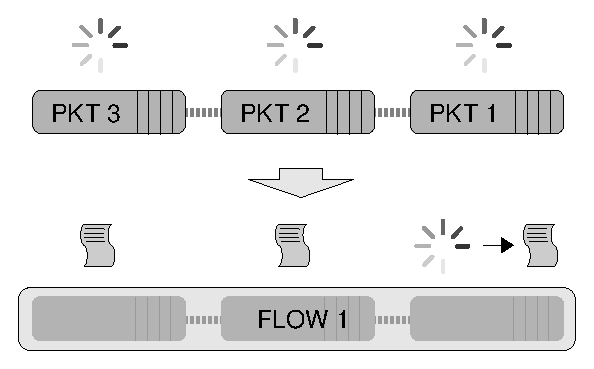
\includegraphics[width=0.70\textwidth]{1-introduccion/graf/packet_vs_flow-crop.eps}
  \caption{Agregación en flujos}
  \label{fig:flow}
\end{figure}


Las VLANs son redes lógicamente independientes que están conectadas a un mismo conmutador físico. Su funcionamiento se basa en un etiquetado dentro de las tramas de enlace de datos.


\begin{figure}[h]
  \centering
	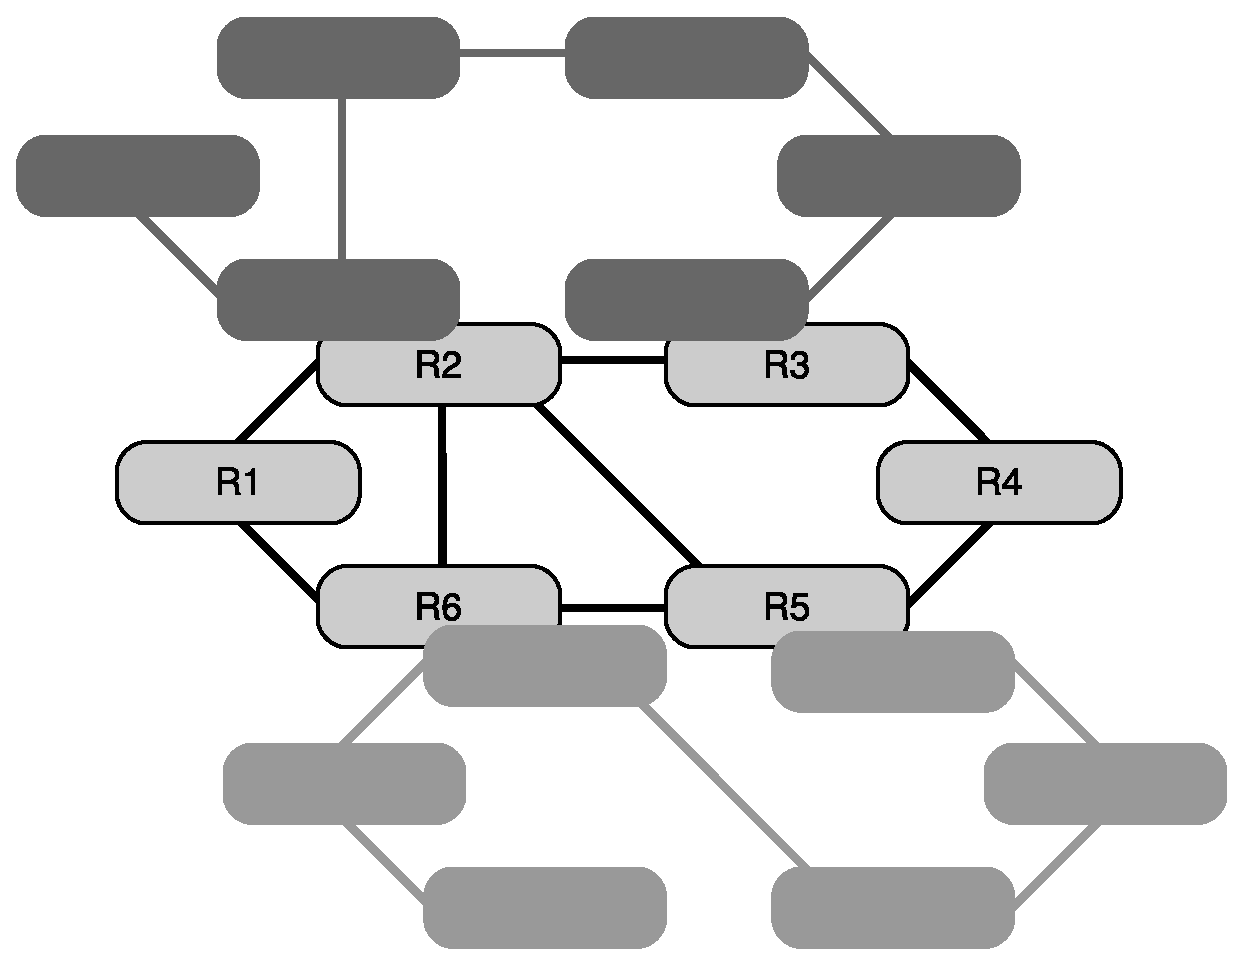
\includegraphics[width=0.70\textwidth]{1-introduccion/graf/network_virtualization_2.eps}
  \caption{Virtualización de redes}
  \label{fig:virt}
\end{figure}


%\subsection{Lógica reconfigurable como respuesta}

En cuanto al Hardware necesario para hacer frente a esta brecha entre la necesidad de procesar el flujo creciente de datos de la red y la capacidad de hacerlo, se busca contar con soluciones que permitan generar respuestas especificas de manera flexible, en el menor tiempo y con el mejor rendimiento posible.

Las tecnologías que en la actualidad son usadas para implementar soluciones a estos problemas, son tres:

Los Circuitos de Propósito Específico (ASICs), que están formados por cientos de bloques especializados trabajando en paralelo. Aunque cuentan con un altísimo desempeño, tienen un alto costo inicial y el tiempo para desarrollarlo es grande.

Los Procesadores de Red (NPs), son procesadores específicos para este tipo de problemas, cuentan con múltiples elementos de procesamiento, buena performance para ciertas tareas, aunque tienen dificultades a la hora de la portabilidad y sus interfaces son propietarias en casi todos los casos.
\begin{figure}[h]
  \centering
      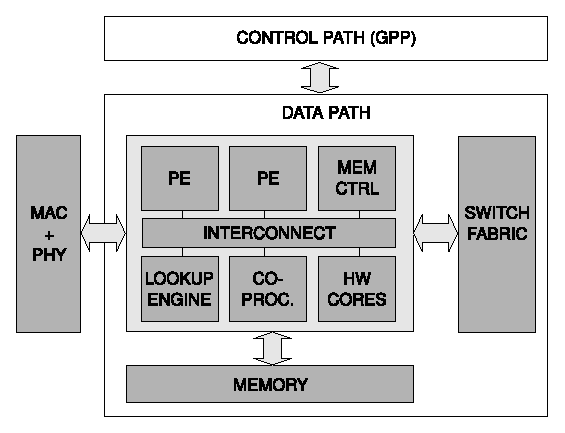
\includegraphics[width=0.5\textwidth]{1-introduccion/graf/NP_based.eps}
  \caption{Solución basada en NP}
  \label{fig:diseno}
\end{figure}
\newpage

Los Procesadores de Propósito General (GPPs), utilizan la arquitectura propia de la PC y la adaptan al procesamiento de la red mediante un software especializado. Aunque esta solución es muy popular por su flexibilidad y su bajo costo, las transiciones con memoria RAM mediante un bus compartido y la naturaleza secuencial de los GPPs son factores limitantes a tener en cuenta. 
 \begin{figure}[h]
  \centering
      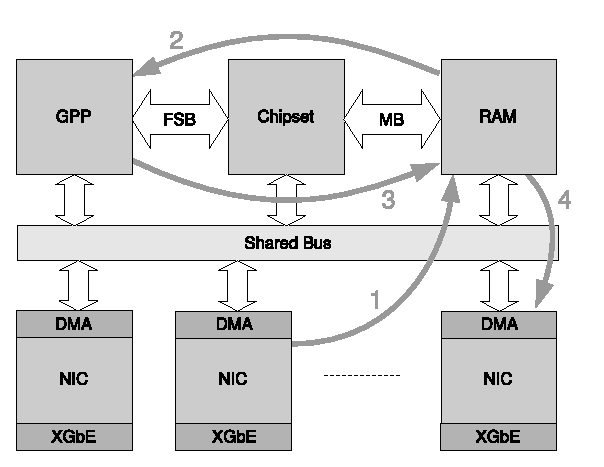
\includegraphics[width=0.5\textwidth]{1-introduccion/graf/GPP_based.eps}
  \caption{Solución basada en GPP}
  \label{fig:diseno}
\end{figure}

Las tecnologías actuales, por las razones anteriormente mencionadas, están alcanzando su limite y es necesario encontrar tecnologías que las reemplacen, para poder satisfacer los requerimientos actuales de las redes. 

Las FPGA(field-programmable gate array) son dispositivos de lógica reconfigurable que es posible programar, una o varias veces, usando un lenguaje de Descripcion de hardware(HDL). Las FPGAs se utilizan en aplicaciones similares a los ASICs sin embargo son más lentas, tienen un mayor consumo de potencia y no pueden abarcar sistemas tan complejos como ellos. A pesar de esto, tienen un flujo de diseño flexible, sus costes de desarrollo y adquisición son mucho menores para pequeñas cantidades de dispositivos y el tiempo de desarrollo es también menor.

%\subsubsection{FPGA como plataforma para SoC}

Los Sistemas en un Chip (SoC) son circuitos integrados que contienen todo, o la mayoría, de los módulos que corresponden a un sistema informático o electrónico en un solo componente. Son usados especialmente en el área de sistemas embebidos. Los microcontroladores son técnicamente SoC, pero se considera que los SoC tienen procesadores mas potentes y pueden correr aplicaciones mas complejas, para lo cual necesitan mayor cantidad de memoria que suele estar disponible como chips externos. 

Gracias a la disponibilidad en la ultima década de Soft-Core CPUs y otros Soft IP, se ha producido un punto de inflección en el uso de FPGAs como plataforma para SoC; Mezcla de logros técnicos y fuerzas de mercado, varios fabricantes como Altera, Cypress Semiconductor, Intel y Xilinx anunciaron la comercialización de FPGA con facilidades para el desarrollo de SoC.

Estos avances que simplifican el desarrollo de SoC, la flexibilidad en el flujo de diseño y el prototipado rápido son las condiciones que posicionan a las FPGA como la herramienta indicada para atacar un problema tan complejo como la clasificación de paquetes. 

 \begin{figure}[h]
  \centering
	 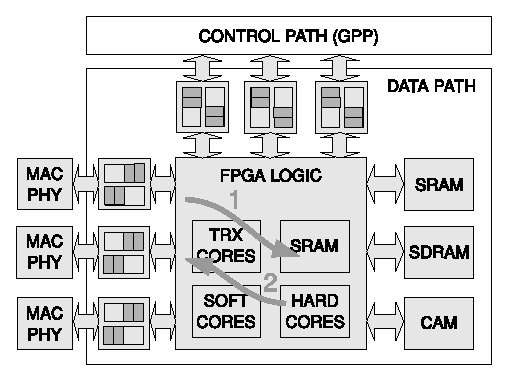
\includegraphics[width=0.5\textwidth]{1-introduccion/graf/FPGA_based.eps}
  \caption{Solución basada en FPGA}
  \label{fig:diseno}
\end{figure}

     




\section{Problema Marco}
\begin{comment}
\subsubsection{Datagrama IP}

\begin{figure}[h]
  \centering
	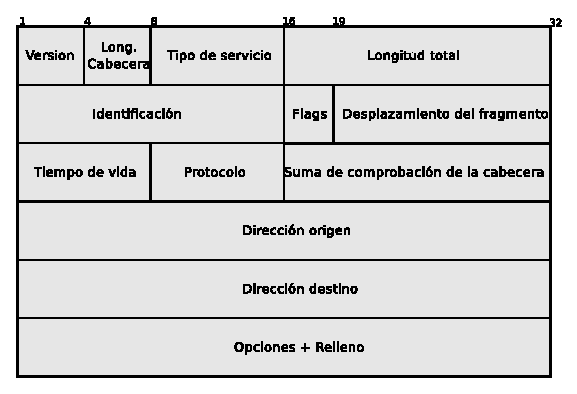
\includegraphics[width=1\textwidth]{2-sistema/graf/ip.eps}
  \caption{Formato de datagrama IP}
  \label{fig:ip}
\end{figure}

La PDU del protocolo IP se denomina \textit{datagrama IP} y se compone de los siguientes campos:
\begin{itemize}
	\item Versión: indica la versión del protocolo.
	\item Longitud de la cabecera: longitud de la cabecera expresada en palabras de 32 bits.
	\item Tipo de servicio: especifica los parámetros de fiabilidad, prioridad, retardo y rendimiento.
	\item Longitud total: longitud total del datagrama en Bytes.
	\item Identificador: un número de secuencia que, junto a la dirección origen y destino y el protocolo usuario, se utiliza para identificar de forma unívoca al datagrama.
	\item Flags: son 3 bits de los cuales solo 2 están definidos. El bit de \textit{no fragmentación} prohíbe la fragmentación cuando está puesto a 1. El bit de \textit{Más datos} se utiliza para fragmentación y reensamblado.
	\item Desplazamiento del fragmento: indica el lugar donde se sitúa el fragmento dentro del datagrama original, medido en unidades de 64 bits.
	\item Tiempo de vida: en cada enrutador se decrementa en 1 unidad. Tiene como fin evitar que un datagrama se quede dando vueltas para siempre en la red.
	\item Protocolo: especifica a que protocolo del nivel de transporte corresponde el datagrama.
	\item Suma de comprobación de la cabecera: Es el complemento a uno de la suma en complemento a uno de todas las palabras de 16 bits de la cabecera.
	\item Dirección origen: codificada para permitir una asignación variable de bits para especificar la red y el sistema final conectado a la red especificada.
	\item Dirección destino: igual que el campo anterior.
	\item Opciones: contiene las opciones solicitadas por el usuario que envía los datos.
	\item Relleno: se usa para asegurar que la cabecera del datagrama tenga una longitud múltiplo de 31 bits.
	\item Datos: debe tener una longitud múltiplo de 8 bits.
\end{itemize}

\subsubsection{Dirección IP}

Es un número de 32 bit que identifica un dispositivo dentro de una red que utilice el protocolo IP. Las direcciones IP se suelen representar por cuatro números decimales separados por puntos, que equivalen al valor de cada uno de los cuatro bytes que componen la dirección.

Como ocurre en la mayoría de las redes las direcciones IP tienen una estructura jerárquica. Una parte de la dirección corresponde a la red, y la otra al host dentro de la red. Cuando un dispositivo de enrutamiento recibe un datagrama por una de sus interfaces compara la parte de red de la dirección con las entradas contenidas en sus tablas (que normalmente sólo contienen direcciones de red, no de host) y envía el datagrama por la interfaz correspondiente.

Los bits que corresponden a la parte de red conforman lo que se denomina \textit{prefijo de red}.

Existen 3 maneras de representar un prefijo de red:

\begin{itemize}
	\item Binario con asterisco: por ejemplo, el prefijo 132.239 se denotaría 1000010011101111* (dado que 132 es en binario 10000100 y 239 es 11101111). El asterisco al final denota que los bits restantes pueden ser de cualquier valor.
	\item Notación A/L, donde A es una dirección IP y L es la longitud del prefijo. Siguiendo el ejemplo anterior, la notación sería 132.239.0.0/16.
	\item Notación máscara: pe utiliza una dirección de red y una máscara en vez de un prefijo explícito. De esta manera, volviendo al ejemplo anteriormente mencionado, éste puede expresarse como 132.239.0.0 con máscara 255.255.0.0
\end{itemize}
\end{comment}

La necesidad de procesar cada vez más paquetes de datos lleva a lo que se conoce como \textit{clasificación}. Ésta consiste en la categorización de paquetes en flujos se denomina. Se efectúa en base a un número de campos en la cabecera del paquete, tales como la dirección de origen/destino, puerto de origen/destino, tipo de servicio (TOS), etc. En general, para una clasificación basada en N campos, se dice que la misma es N-dimensional (o multidimensional). El propósito de la misma es clasificar paquetes de acuerdo a un conjunto de reglas dado.

Cada regla \textbf{R} tiene \textbf{F} componentes y el $ f^{vo} $ componente de \textbf{R}, denotado como \textbf{R[f]} es una \textit{expresión de correspondencia de rango} en el $ f^{vo} $ campo del paquete. Si para todo \textit{f} $ \in $ [1, \textit{f}] el $ f^{vo} $ campo de la cabecera de un paquete \textbf{P} satisface la expresión de rango \textbf{R[f]}, \textbf{P} se corresponde con \textbf{R}.

Un caso particular de clasificación unidimensional es lo que se conoce como IP Lookup. Es el caso que se abordará en este trabajo.

\subsubsection{Dirección IP}

Es un número de 32 bit que identifica un dispositivo dentro de una red que utilice el protocolo IP. Las direcciones IP se suelen representar por cuatro números decimales separados por puntos, que equivalen al valor de cada uno de los cuatro bytes que componen la dirección.

Como ocurre en la mayoría de las redes las direcciones IP tienen una estructura jerárquica. Una parte de la dirección corresponde a la red, y la otra al host dentro de la red. Cuando un dispositivo de enrutamiento recibe un datagrama por una de sus interfaces compara la parte de red de la dirección con las entradas contenidas en sus tablas (que normalmente sólo contienen direcciones de red, no de host) y envía el datagrama por la interfaz correspondiente.

Los bits que corresponden a la parte de red conforman lo que se denomina \textit{prefijo de red}.

Existen 3 maneras de representar un prefijo de red:

\begin{itemize}
	\item Binario con asterisco: por ejemplo, el prefijo 132.239 se denotaría 1000010011101111* (dado que 132 es en binario 10000100 y 239 es 11101111). El asterisco al final denota que los bits restantes pueden ser de cualquier valor.
	\item Notación A/L, donde A es una dirección IP y L es la longitud del prefijo. Siguiendo el ejemplo anterior, la notación sería 132.239.0.0/16.
	\item Notación máscara: pe utiliza una dirección de red y una máscara en vez de un prefijo explícito. De esta manera, volviendo al ejemplo anteriormente mencionado, éste puede expresarse como 132.239.0.0 con máscara 255.255.0.0
\end{itemize}

\subsubsection{IP Lookup}

El procedimiento que se lleva acabo en un dispositivo de enrutamiento podría describirse de la siguiente manera:

Un paquete llega por una interfaz de entrada. Éste porta una dirección IP determinada. El dispositivo consulta una tabla para determinar la interfaz de salida para el paquete en cuestión. Dicha tabla contiene un conjunto de prefijos con sus correspondientes interfaces de salida. El paquete es correspondido con el prefijo más largo que esté contenido en la dirección de destino y luego es redirigido  a la correspondiente interfaz de salida. Esta tarea de determinar el enlace de salida es denominada \textit{Búsqueda de dirección (address lookup).}

En la figura ~\ref{fig:prefijos} puede observarse una dirección IP como así también 3 prefijos de diferentes longitudes. Tanto éstos como la dirección están representados por sus bits. En el procedimiento de address lookup la interfaz seleccionada sería aquella asociada al prefijo más largo.

 \begin{figure}[h]
  \centering
	 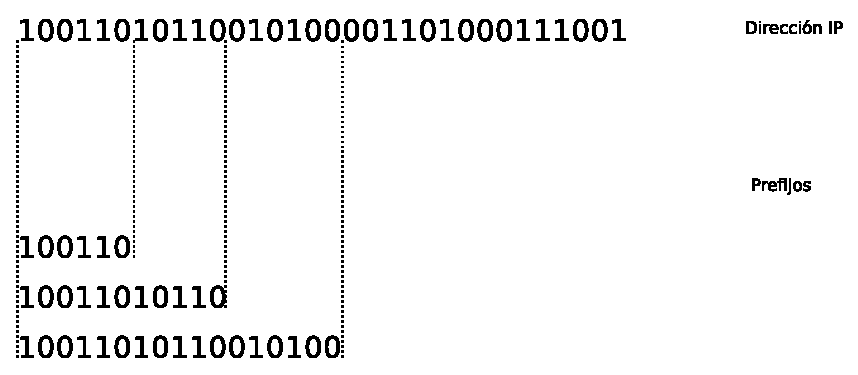
\includegraphics[width=0.7\textwidth]{1-introduccion/graf/prefijos.eps}
  \caption{Dirección IP y prefijos de diferente longitud}
  \label{fig:prefijos}
\end{figure}



\section{Objetivos}
\subsection{Objetivos Generales}
Teniendo en cuenta los problemas planteados, el objetivo general de este proyecto es estudiar los diversos algoritmos de clasificación de paquetes para poder encontrar las limitaciones en la implementación de los mismos tanto en software como en hardware. 
En Particular, se pretende considerar una plataforma de lógica reconfigurable que permite integrar arquitecturas de Hardware con Software embebido.

\subsection{Objetivos Específicos}

    \begin{itemize}     

     	\item Diseñar un sistema embebido que realice la clasificación unidimensional de paquetes mediante una arquitectura mixta, Hardware-Software
	\item Implementar dicho sistema en hardware reconfigurable
	\item Implementar al menos 2 algoritmos conocidos y analizar su performance
	\item Sugerir mejoras en la implementación de los mismos   

\end{itemize}


\section{Organización}

En el Capitulo 2 se estudiara, a nivel funcional, una solución propuesta para este tipo de problemas. A continuación se presentara de manera detallada la Arquitectura digital de los módulos que componen el sistema. En el Capitulo 4 se describirá la metodología y los recursos utilizados para implementar este proyecto y en el Capitulo 5 se presentan las diferentes curvas resultantes de la ejecución de esta implementación.





%\section{Distribucion Lineal}

\chapter{Sistema}

Entre de dispositivos que realizan la clasificación de paquetes se encuentran soluciones implementadas de manera completa en hardware, FPGA, ASIC u otra plataforma, como por ejemplo NetFPGA\cite{netfpga}, o implementadas, procesador de propósito general mediante, completamente en software, que es el caso de Click\cite{click}. La intención de este proyecto integrador, como puede verse de manera gráfica en la figura~\ref{fig:hwsw}, es complementar las ventajas de ambos mundos maximizándolas y reduciendo así las desventajas de utilizar el hardware o el software por separado. 


 \begin{figure}[h]
  \centering
	 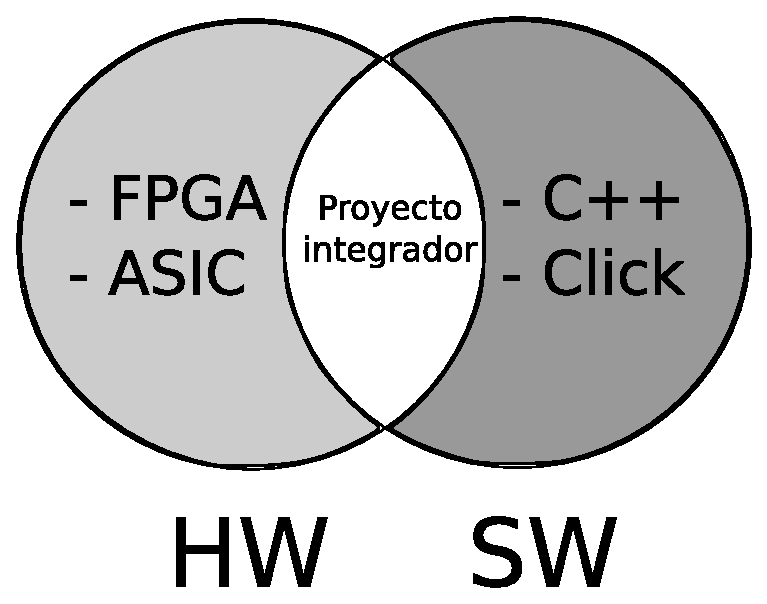
\includegraphics[width=0.6\textwidth]{2-sistema/graf/interseccion.eps}
  \caption{Arquitectura mixta}
  \label{fig:hwsw}
\end{figure}


\section{Solución propuesta}

Para el problema planteado en el capítulo anterior se propone, de manera funcional, la siguiente solución: 

    \begin{enumerate}
  	\item Un flujo de paquetes llega a la interfaz de red del dispositivo y es necesario clasificarlo en distintos flujos para que sea redireccionado.
	\item Se almacenan los paquetes en un buffer según el orden de llegada.
	\item Se extrae el primer paquete y se toma la información que pertenece a la cabecera; La información completa del paquete queda en espera.
	\item Se envía la cabecera al microprocesador.
	\item El microprocesador aplica un algoritmo de clasificación a cierta información de la cabecera y reenvía los resultados al hardware. 
	\item Se envía el paquete a la interfaz de salida, anexándole a cada palabra un tag adjunto con el resultado de la clasificación.
    \end{enumerate}

\section{Esquema propuesto}
Para implementar la solución se propone el hardware descripto en el diagrama de la figura~\ref{fig:solucion}
 \begin{figure}[h]
  \centering
	 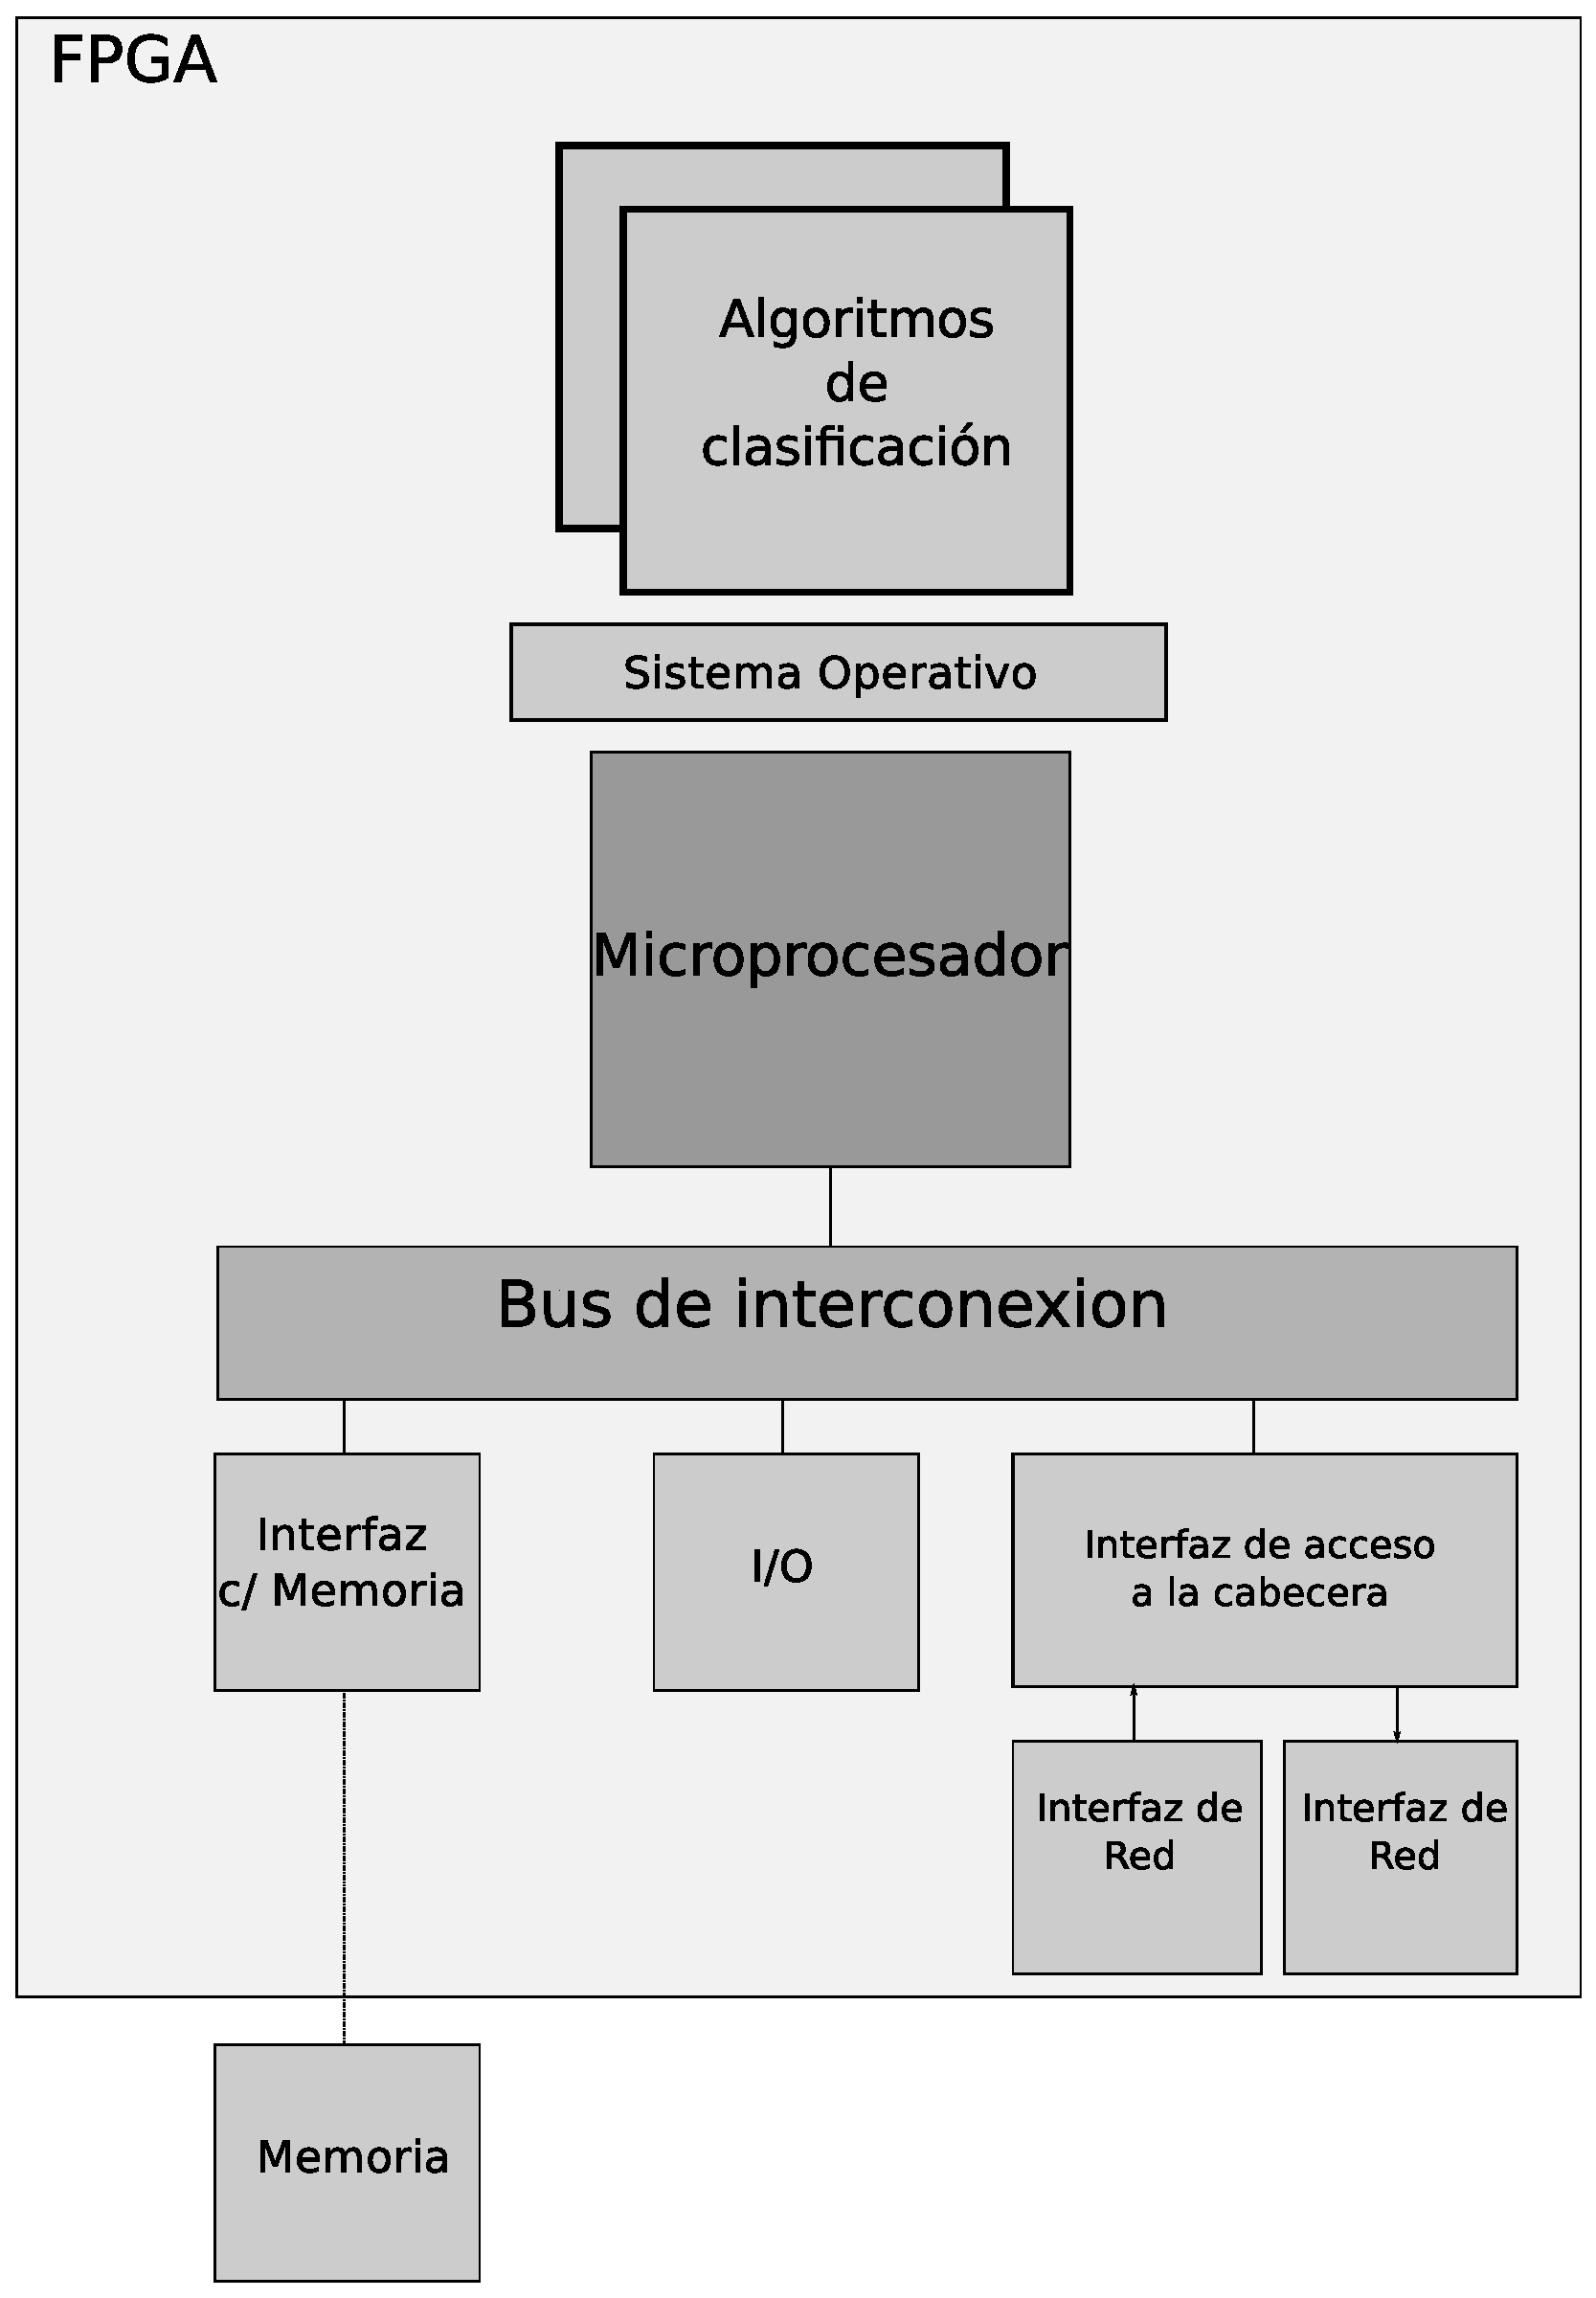
\includegraphics[width=0.6\textwidth]{2-sistema/graf/solucion.eps}
  \caption{Diagrama de la arquitectura propuesta}
  \label{fig:solucion}
\end{figure}

De los módulos mencionados, es necesario poner especial atención en el diseño de la interfaz de acceso a la cabecera.

\subsection{Interfaz de acceso a la cabecera}
Este módulo tiene como función acceder a los campos que conforman la cabecera IP en los paquetes entrantes. La información recolectada es enviada al microprocesador para que este implemente el software de clasificación.

\newpage

 \begin{figure}[h]
  \centering
	 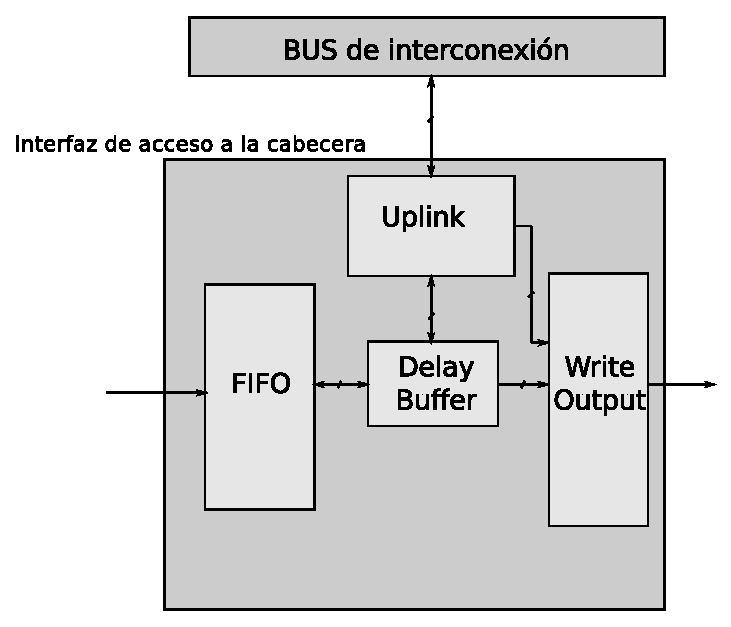
\includegraphics[width=0.6\textwidth]{2-sistema/graf/modulo.eps}
  \caption{Interfaz de acceso a la cabecera}
  \label{fig:inter}
\end{figure}



%\subsection{Descripción funcional}

A continuación se describe funcionalmente cada uno de los bloques que conforma la interfaz, ilustrada en la figura~\ref{fig:inter}
\subsubsection{Cola de espera FIFO\textit{(First in First out)}}
A la entrada del módulo se encuentra una FIFO que se encarga de almacenar y poner a disposición en orden de llegada los datos que emite el generador. Además, para poder manipular los paquetes, la FIFO debe almacenar toda la información de control disponible a su entrada.
Este módulo también debe permitir la parametrización en la mayor cantidad de sentidos posibles, especialmente se desea poder configurar la cantidad de palabras a almacenar, ya que la memoria dentro de un FPGA es un recurso crítico y se desea encontrar la mejor relación entre rendimiento y consumo de recursos.

\subsubsection{Delay Buffer}
Este componente será el encargado de ir tomando los datos desde la FIFO y de detectar el inicio y finalización de un paquete. Además deberá mantener almacenada la cabecera del paquete mientras el software toma una decisión. En este módulo es deseable configurar la cantidad de palabras que se considerarán parte de la cabecera y que serán enviadas al microprocesador.

\subsubsection{Uplink}
Este módulo es el encargado de gestionar las transacciones con el microprocesador. Para ello debe entender las señales que utiliza el bus y poder interrumpir al procesador para enviarle los datos cuando estos estén disponibles. Asimismo cuando el procesador responde con el resultado de la clasificación, Uplink lo almacena y lo envía al módulo Write output para que este escriba el resultado de la clasificación en la etiqueta anexa al paquete correspondiente.
Eventualmente se desarrollaran varias versiones de este módulo, que envíen toda la cabecera o una parte selectiva de ella buscando optimizar el rendimiento.

\subsubsection{Write Output}
Para finalizar este módulo toma la salida de Delay Buffer y escribe el resultado que le envía Uplink en la etiqueta que se encuentra anexa a cada una de las palabras del paquete.

\section{Algoritmos de Clasificación}

Los algoritmos de clasificación de paquetes que se implementaron fueron los siguientes:

\subsection{Búsqueda lineal}

El esquema más simple de lookup consiste en una tabla, donde cada entrada contiene un prefijo (expresado en notación máscara) mas un identificador de enlace de salida. Cuando llega un paquete se examina su dirección IP y se va comparando con cada uno de los prefijos almacenados. Para que exista correspondencia debe existir igualdad bit a bit entre el prefijo y la dirección IP. Si esto se cumple para varios prefijos, se opta por el más largo de ellos y el paquete se expide por el enlace asociado a dicho prefijo.
Para optimizar este esquema, los prefijos se almacenan en orden decreciente de longitud, como se muestra en la figura~\ref{fig:linear}, de manera que al encontrar una coincidencia no sea necesario seguir buscando en el resto de la tabla. 

\begin{figure}[h]
  \centering
	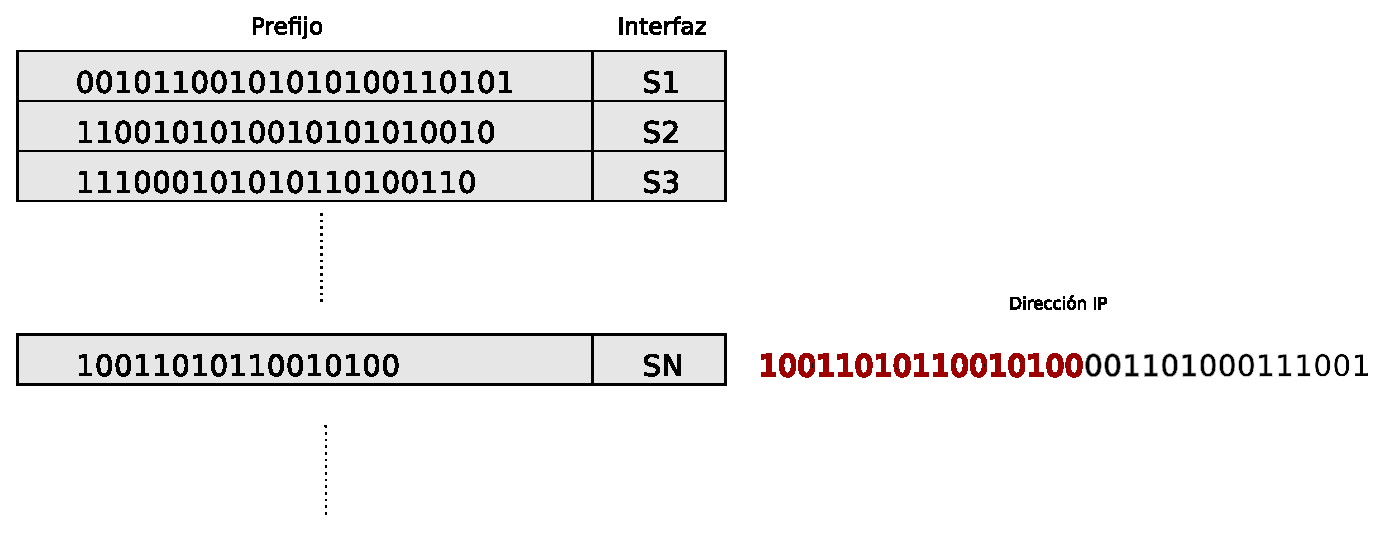
\includegraphics[width=0.80\textwidth]{2-sistema/graf/linear.eps}
  \caption{Búsqueda lineal}
  \label{fig:linear}
\end{figure}

\newpage
\subsection {Unibit tries}

Un Unibit trie es un árbol en el cual cada nodo contiene un \textit{puntero-cero }y un \textit{puntero-uno}. Partiendo del nodo raíz, todos los prefijos que comienzan con 0 son almacenados en el subárbol apuntado por el puntero-cero y aquellos que comienzan con 1 se almacenan en el subárbol apuntado por el puntero-uno.Cada subárbol es construido recursivamente de manera similar usando los bits restantes de cada uno de los prefijos.
Considerar la siguiente tabla de enrutamiento:
\begin{table}[h]
\begin{center}
	\begin{tabular}{|c|c|} \hline
		\textbf{Prefijo} & \textbf{Enlace de salida} \\ \hline
		101* & S1 \\
		111* & S2 \\
		11001* & S3 \\
		1* & S4 \\
		0* & S5 \\
		1000* & S6 \\
		100000* & S7 \\
		100* & S8 \\
		110* & S9 \\	\hline
	\end{tabular}
	\caption{Prefijos y enlaces de salida}
	\label{tab:prefgw}	
\end{center}
\end{table}



A la misma le corresponde la representación en Unibit trie de la figura~\ref{fig:trie}.
Sea una dirección de destino \textit{D}. Para efectuar la búsqueda del prefijo más largo, los bits de \textit{D} son usados para trazar un camino a lo largo del trie. Dicho camino comienza en el nodo raíz y continúa hasta encontrar un puntero vacío o un nodo vacío. Durante el recorrido a través del trie, el algoritmo mantiene un registro del último enlace encontrado en un nodo del camino recorrido (que es el mas largo hasta el momento). En el caso que la búsqueda terminara éste es el prefijo retornado.

\begin{figure}[h]
  \centering
	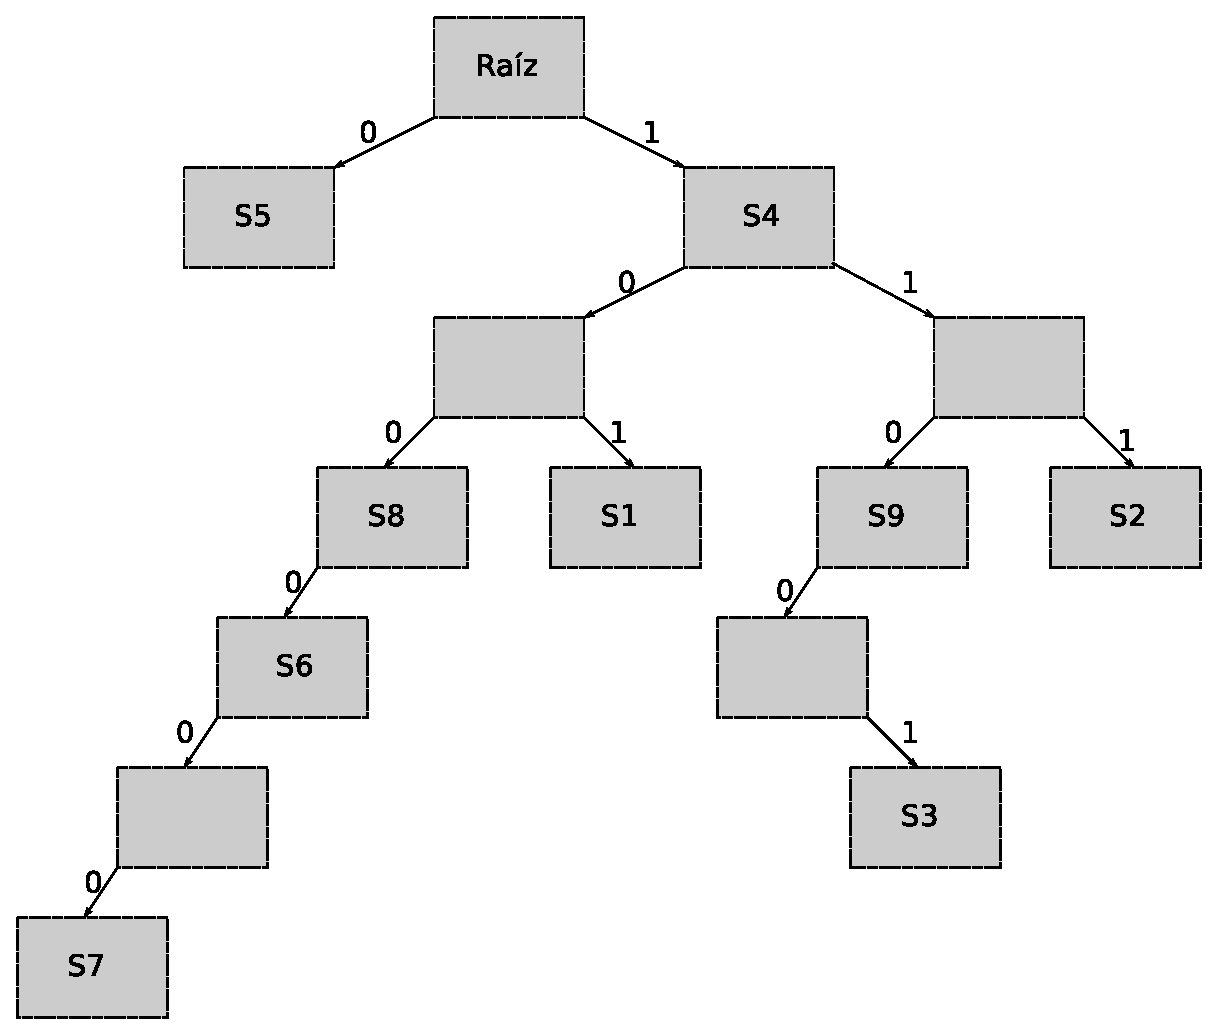
\includegraphics[width=0.80\textwidth]{2-sistema/graf/trie.eps}
  \caption{Unibit trie}
  \label{fig:trie}
\end{figure}


 
\chapter{Arquitectura}
En este capitulos se detallara la arquitectura del proyecto en general, poniendo foco en la seleccion adecuada de las tecnologias a utilizar y completando mas detalladamente el diseño obtenida en el capitulo anterior.

\section{Procesador Embebido}

Como se dijo en el capitulo 2, los microprocesadores embebidos en logica reprogramable se clasifican, basicamente, en dos tipos Hardcore y Softcore. Aunque los Hardcores ofrecen unas mejores prestaciones existen muy pocos dispositivos en el mercado que ofrecen este tipo de modulos y, en general, el costo de este tipo de dispositivos es mayor que el de uno que no cuenta con un hardcore. Por esta razones de ahora en adelante se limitara el estudio a softcores, siempre buscando que lo implementado siga los principios del diseño modular a los fines de facilitar la portabilidad.
\subsection{Estudio de los softcores disponibles}
Los SoftCores pueden ser clasificados en tres tipos segun su origen

\begin{itemize}
	\item Provistos por los fabricantes de las FPGA
	\item Provistos por empresas distribuidoras de bloques IP(Intelectual Property)
	\item Provistos por la comunidad Open Source
\end{itemize}

\subsubsection{Provistos por los fabricantes de las FPGA}
Xilinx y Altera, los dos mayores fabricantes de FPGA, proveen un Softcore para integrar en sus dispositivos. La ventaja natural de este tipo de core es que se encuentran altamente integrados en las herramientas de desarrollo de dichos fabricantes, permitiendo montar un sistema embebido en minutos de manera grafica e intuitiva. Ademas estan a disposición del usuario una buena cantidad de  modulos IP para anexar al procesador y aumentar asi sus funcionalidades. 

Dentro de las desventajas esta el hecho de que son dependientes de la plataforma y no es posible implementar el core propietario de Altera en un dispositivo Xilinx, y viseversa. Ademas se debe pagar una licencia por el uso de estos cores y no se cuenta con la posibilidad de observar o modificar el codigo de los mismos. 

Xilinx ofrece a los usuarios de sus dispositivos el MicroBlaze, un procesador RISC de 32 bits con una arquitectura muy similar al MIPS DLX. A nivel herramientas de desarrollo la empresa provee el "Xilinx's EDK(Embedded Development Kit)" que permite generar un sistema embebido completo con las interconexiones necesarias. Es posible correr el sistema operativo GNU/Linux en este tipo de procesador.

Altera por su parte ofrece la linea de Cores NIOS II, tambien RISC de 32 bits, que cuenta en tres variantes principales Nios II Fast, Economy y Standard y dos variantes especializadas Nios II SC core, para aplicaciones militares y aeroespaciales, y DesignWare IP, para implementar en ASIC. Altera provee ademas una interfaz de usuario para la construccion del sistema embebido llamado SOPC que se encuentra integrado a Quartus y ademas el Nios II Embedded Design Suite (EDS) que permite diseñar el software requerido para cada aplicacio. Permite la implementacion del sistema operativo GNU/Linux.

\subsubsection{Provistos por empresas distribuidoras de bloques IP}
Existe una buena cantidad de empresas que se dedican a generar y comercializar bloques de propiedad intelectual (IP Cores o IP Blocks), unidades logicas reusables que son propiedad intelectual de un individuo o empresa.
Varias de estas empresas cuentan con Softcores con distintas capacidades y tecnologias. La ventaja principal esla portabilidad de estos cores entre FPGA de distintos fabricantes. Entre las desventajas podemos nombrar la calidad de la documentacion y la complejidad intrinseca que implica comprender y utilizar una herramienta de desarrollo de un tercero. 

Dentro de los mas conocidos se puede nombrar a la linea Leon de la empresa Aeroflex, LatticeMico32 de Lattice semiconductor o ARM cortex de Freescale. Los IP core pueden estar licenciados de diferentes formas incluidas entre ellas GPL.
 
\subsubsection{Provistos por la comunidad Open Source}
La comunidad open source se ha encargado de producir una buena cantidad de softcores, las capacidades y perfomance de los mismos cubre casi todos los rangos. En la pagina web que lleva una lista de este tipo de proyectos, opencores, se pueden encontrar alrededor de 130 cores. El problema con este tipo de core esta en la poco uniforme calidad de la documentacion y en la calidad dudosa de varios de los cores. Sin embargo la flexibilidad para poder modificar la arquitectura a gusto y el costo cero de implementacion son ventajas nada despreciables de estos productos. 

Se destaca el proyecto Openrisc 1200, que tiene una gran comunidad que lo soporta y algun prestigio ganado en este terreno.


\subsubsection{Tabla comparativa}
																																						 																												
																																								

\begin{table}
	\centering
	\begin{tabular}{|p{1.65cm}|p{1.98cm}|c|p{2.2cm}|p{1.5cm}|c|c|p{1.5cm}|} \hline
		Core & Arquitectura & Licencia & Profundidad del Pipeline & Ciclos por Instruccion & MMU & FPU & FPGA \\ \hline
		MicroBlaze & MicroBlaze & Propietaria & 3,5 & 1 & Opt & Opt & Xilinx\\ \hline
		Nios II/fast & Nios II & Propietaria & 6 & 1 & si & opt & Altera \\ \hline
		Nios II/std & Nios II & Propietaria & 5 & 1 & no & Opt & Altera \\ \hline
		Nios II/econ & Nios II & Propietaria & no & 6 & no & Opt & Altera \\ \hline
		LEON3 & SPARC-v8 & GPL & 7 & 1 & si & si & Xilinx, Altera, Lattice \\ \hline
		OpenRISC 1200 & OpenRISC 1000 & LGPL & 5 & 1 & si & no & Xilinx, Altera, Lattice \\ \hline
		Lattice Mico32 & Lattice Mico32 & Propietaria & 6 & 1 & no & no & Indep. \\ \hline
		Cortex-M1 & ARMv6 & Propietaria & 3 & 1 & no & no & Xilinx, Altera \\ \hline
	\end{tabular}
	\caption{Comparativa softcores}
	\label{tab:comp}
\end{table}


\section{Modulo Gestor de Datos}
\section{Software}

\subsection{NIOS II SBT}

El NIOS II Software Building Tools (o SBT) es un conjunto de utilidades y scripts que sirve para crear y construir aplicaciones embebidas basadas en C/C++, librerías de usuario y paquetes de soporte de placa (board support packages o BSP). 

Puede invocarse desde la IDE Eclipse o desde el intérprete de comandos del NIOS II.

El NIOS II SBT puede crear los siguientes tipos de proyecto:
\begin{itemize}
	\item Aplicación NIOS II: un programa que implementa alguna funcion deseada.
	\item NIOS II BSP: una librería que provee acceso al hardware en el sistema. Brinda un entorno de rutinas a medida para un procesador y, eventualmente, un sistema operativo. 
	\item Librería de usuario: un conjunto de funciones reutilizables. 
\end{itemize}

\subsubsection{Aplicaciones y librerías de usuario}

Para el caso de aplicaciones y librerías de usuario, el SBT genera un makefile privado (denominado \textbf{Makefile}) el cual es usado para construir el proyecto. Al hacer esto se genera un archivo .elf para una aplicación, o .a para una librería. En este último caso, también se produce un makefile público (denominado \textbf{public.mk}), que se incluye en el privado para cualquier aplicación que use la librería de usuario.

Cuando se crea un makefile se provee al SBT con una lista de archivos de código fuente y una referencia al directorio donde se almacena el BSP. Luego, la herramienta examina la extensión de cada archivo fuente para determinar el lenguaje de programación. 

Actualmente, los soportados son:

\begin{itemize}
	\item C (extensión .c).
	\item C++ (extensiones .cpp, .cxx, .cc).
	\item NIOS II Assembler (extensiones .s, .S).
\end{itemize}


\subsubsection{Board Support Packages}

Un BSP es una librería especializada que contiene código de soporte específico del sistema. Aisla la aplicación de los detalles del sistema, tales como mapeo de memoria, dispositivos disponibles y configuración del procesador.

Se compone de:

\begin{itemize}
	\item Capa de abstracción de Hardware (Hardware Abstraction Layer o HAL): Permite al software interactuar con el hardware del sistema. Se describirá en detalle más adelante en este capítulo.
	\item Librería C estándar newlib: ANSI C estándar diseñada para sistemas embebidos.
	\item Drivers de dispositivos: para manejar cada uno de los componentes del sistema.
	\item Paquetes de software opcionales: permiten proveer funcionalidad adicional.
	\item Sistema operativo de tiempo real opcional: implementación de MicroC/OS-II RTOS.
\end{itemize}

\subsubsection{Proceso de construcción del software}

Para crear un proyecto de software se llevan a cabo una serie de pasos:

\begin{enumerate}
	\item Se obtiene el diseño de hardware sobre el cual va a correr el software. Dicha información está almacenada en un archivo de extensión \textbf{.sopcinfo}, el cual es generado por la herramienta SOPC builder.
	\item Se genera el BSP con las características necesarias según las funcionalidades requeridas. También se genera un makefile para dicho paquete.
	\item Opcionalmente, se crea una librería de usuario (junto a su correspondiente makefile).
	\item Se escribe el software de aplicación. Se colecta todo el código fuente, y luego se genera el makefile correspondiente.
	\item Se construye el proyecto.
\end{enumerate}


\subsection {HAL}

La Capa de Abstracción de Hardware \textit{(Hardware Abstraction Layer o HAL)} provee una interfaz simple de drivers de dispositivos para conectar los programas con el hardware subyacente. La API está integrada con la librería estándar ANSI C, lo cual permite al software acceder a los dispositivos mediante el uso de funciones C ampliamente conocidas, tal como printf(), fopen(), fwrite(), etc.

\subsubsection{Servicios}

La HAL provee los siguientes servicios:

\begin{itemize}
	\item Integración con la librería estándar newlib: provee funciones estándar ANSI C de amplio uso.
	\item Drivers de dispositivo: brinda acceso a cada dispositivo en el sistema.
	\item API: proporciona una interfaz estándar consistente a los servicios de la HAL, tales como acceso a dispositivos y manejo de interrupciones.
	\item Inicialización de sistema: Lleva a cabo la inicialización para el procesador y las rutinas antes de ejecutar la función principal (main).
	\item Inicialización de dispositivos: Instancia e inicializa cada uno de los dispositivos del sistema antes de que se ejecute la función main.
\end{itemize}

La figura ~\ref{fig:hal} muestra las capas de un sistema basado en la HAL, desde el nivel de hardware hasta el programa de usuario.

\begin{figure}[H]
  \centering
	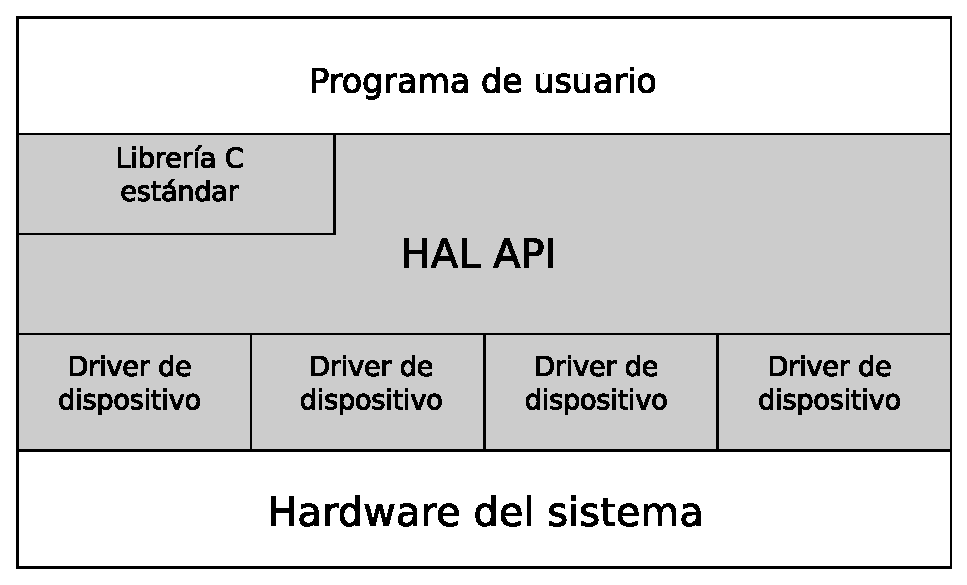
\includegraphics[width=0.80\textwidth]{3-arquitectura/graf/hal.eps}
  \caption{Capas de un sistema basado en la HAL.}
  \label{fig:hal}
\end{figure}

\subsubsection{Modelos de dispositivos genéricos}

La HAL provee modelos de dispositivos genéricos para diversos tipos de periféricos que se encuentran en sistemas embebidos, tales como timers, interfaces Ethernet y dispositivos de I/O que transmiten datos de caracter. Estos modelos permiten escribir programas usando una API consistente sin preocuparse por el hardware subyacente.

Los tipos de periféricos cubiertos son:

\begin{itemize}
	\item Dispositivos de caracter: envían y/o reciben caracteres en forma serial, como ser una UART.
	\item Timers: dispositivos que llevan la cuenta de los tics de un clock y pueden generar interrupciones periódicas.
	\item Subsistemas de archivos: un mecanismo para acceder a archivos almacenados en dispositivos físicos. Dependiendo de la implementación interna, el driver del subsistema de archivos podría acceder a los dispositivos subyacentes en forma directa o usar un driver aparte.
	\item Dispositivos Ethernet: proveen acceso a una conexión Ethernet para una pila de red, tal como la NicheStack® TCP/IP Stack, provista por Altera.
	\item Dispositivos DMA: periféricos que llevan a cabo una gran cantidad de transacciones de datos. El origen y destino pueden ser la propia memoria o algún otro dispositivo.
	\item Dispositivos con memoria flash: periféricos con memoria no volátil que utilizan un protocolo especial de programación para almacenar datos.
\end{itemize}

Todos los periféricos, ya sean de Altera o de terceros, deben proveer un archivo de cabecera que defina la interfaz de bajo nivel del dispositivo con el hardware. 

Ciertos dispositivos tienen características específicas de hardware con requierimientos de uso que no se adaptan bien a una API de propósito general. La HAL maneja dichos requerimientos mediante la función ioctl(), cuyas opciones dependerán del periférico en cuestión.

Algunos periféricos proveen funciones de acceso dedicadas que no están basadas en el modelo genérico de la HAL. En ese caso, se debe proveer un archivo de cabecera con dichas funciones.


\subsubsection{Librería C estándar : newlib}
La HAL integra su entorno de rutinas con una implementación open-source de la librería C estándar:\textbf{ newlib}. La misma está hecha para ser utilizada en sistemas embebidos. 

\subsubsection{La HAL dentro de un proyecto de software}
La creación y administración de proyectos basados en la HAL están altamente ligadas al NIOS II SBT

\begin{figure}[h]
  \centering
	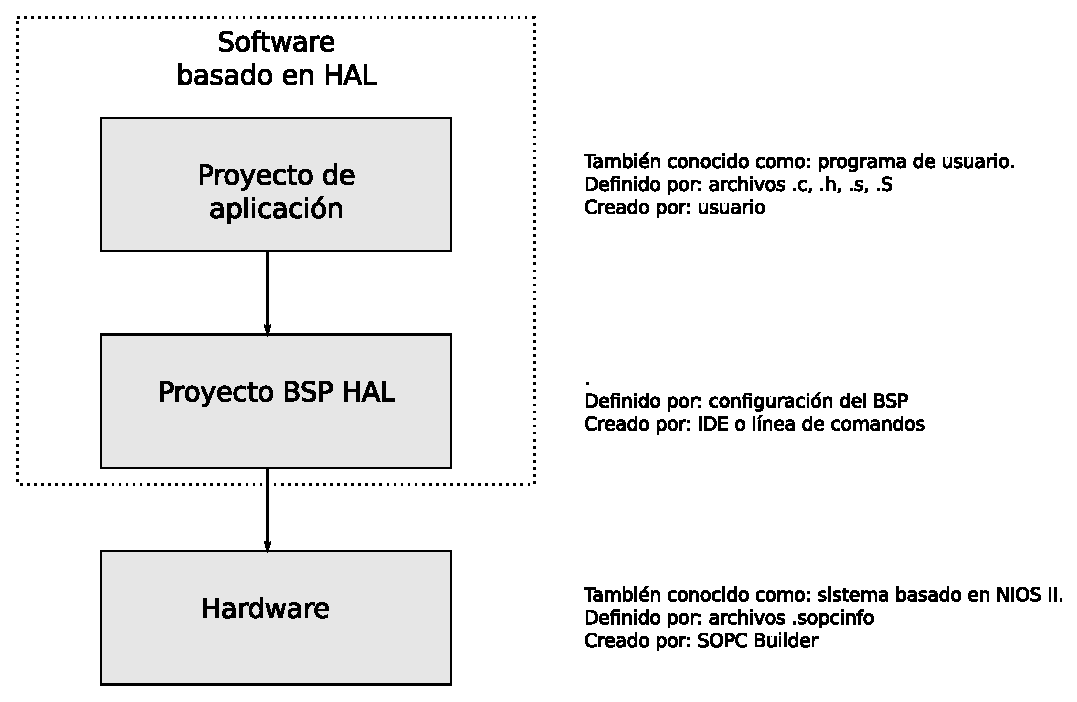
\includegraphics[width=0.90\textwidth]{3-arquitectura/graf/halsof.eps}
  \caption{Capas de un programa basado en HAL}
  \label{fig:halsof}
\end{figure}

La figura ~\ref{fig:halsof} muestra el diagrama en bloques de un software basado en la HAL. Todo programa de este tipo consta de dos proyectos. El ćodigo de aplicación específico se encuentra en uno de ellos, el cual depende a su vez de otro proyecto BSP separado.

EL primero contiene todo el código que el programador desarrolla. El segundo, toda la información necesaria para la interacción hardware-software. Este último a su vez depende del hardware del sistema, cuya información se encuentra en un archivo generado por la herramienta SOPC Builder.

\subsubsection{El archivo de descripción del sistema (system.h)}
El archivo system.h provee una descripción completa del software del sistema basado en NIOS II. Describe cada periférico e incluye:

\begin{itemize}
	\item La configuración de hardware del periférico.
	\item La dirección base.
	\item Información IRQ (si es necesario).
	\item Un nombre simbólico para el periférico.
\end{itemize}

El SBT genera un archivo \textbf{system.h} para cada proyecto BSP, cuyo contenido dependerá del archivo .sopcinfo mencionado anteriormente en este capítulo.

\subsubsection{Acceso al hardware}
El software accede al hardware a través de macros que abstraen la interfaz mapeada en memoria al dispositivo. Todos los componentes proveen un directorio que define el hardware y el software del periférico en cuestión. En esta carpeta se encuentra un archivo de cabecera que define la interfaz con el hardware y su nombre es $<componente>$\_regs.h, el cual se incluye en el subdirectorio inc. Por ejemplo, el componente JTAG UART define su interfaz en el archivo $<Directorio Instalacion Altera>$/ip/altera/sopc\_builder\_ip/

altera\_avalon\_jtag\_uart/inc/altera\_avalon\_jtag\_uart\_regs.h.

El archivo de cabecera \_regs.h define las siguientes macros de acceso para el componente:
\begin{itemize}
	\item Macros de acceso a registros que proveen operaciones de lectura/escritura. Éstas son:
	\begin{itemize}
		\item IORD\_$<NombreDelComponente>$\_$<NombreDelRegistro>$ ($<DireccionBaseDelComponente>$).
		\item IOWR\_$<NombreDelComponente>$\_$<NombreDelRegistro>$ ($<DireccionBaseDelComponente>$, $<Dato>$).
	\end{itemize}
	\item Macros de direccionamiento de registro, que retornan las direcciones físicas de cada uno de ellos. La dirección devuelta es la dirección base del componente + el valor de desplazamiento de registro especificado. Esta macro tiene el nombre de esta forma:
	\begin{itemize}
		\item IOADDR\_$<NombreDelComponente>$\_$<NombreDelRegistro>$ ($<DireccionBaseDelComponente>$).
	\end{itemize}
	\item Máscaras a nivel de bits. Estas macros tienen los siguientes nombres:
	\begin{itemize}
		\item $<NombreDelComponente>$\_$<NombreDelRegistro>$\_$<NombreDelCampo>$\_MSK : Máscara de bit de un campo.
		\item $<NombreDelComponente>$\_$<NombreDelRegistro>$\_$<NombreDelCampo>$\_OFST : Desplazamiento de bit del el comienzo del campo.
	\end{itemize}
\end{itemize}

Cabe mencionar que las los valores leídos/escritos mediante las macros de acceso a registro (IORD e IOWR) no trabajan con la caché del microprocesador.



La razón de utilizar la HAL en vez de un sistema operativo, yace principalmente en la mayor simplicidad de uso que ésta presenta. En el caso de haber optado por el segundo enfoque hubiese sido necesario el desarrollo de drivers para el manejo de los dispositivos, con la complejidad que ello implica. La HAL, por otra parte, ofrece un conjunto de funciones de la librería estándar ANSI C para la interacción con el hardware del diseño, lo cual hace que dicha tarea sea significativamente más simple.



\subsection {Algoritmos de clasificación}

Se implementaron 2 algoritmos de clasificacion: Busqueda lineal y Busqueda en árbol unibit.

El software utilizado para realizar las pruebas consistió en 2 proyectos por separado. Uno para cada tipo de búsqueda en la tabla.

El mismo fue desarrollado en lenguaje c++, por presentar éste ciertas facilidades para las implementaciones llevadas a cabo. Puntualmente se sacó ventaja de un STL container (list) para implementar la búsqueda lineal. La característica utilizada en este caso fue el ordenamiento de la lista con sólo una llamada a función.

Para efectuar el intercambio de datos con el hardware se hizo uso de las macros IOWR e IORD, las cuales escriben y leen respectivamente los datos hacia/desde un componente conectado al bus Avalon MM. La razón de haber usado dichas macros yace en el hecho de que las mismas no son puestas en caché. Esta característica se torna indispensable en este diseño, ya que en el mismo no se puede leer un dato sin saber si está verdaderamente disponible en el bus.


\subsubsection {Búsqueda lineal}

Se implementó en una lista enlazada, creada a partir del template list de c++. Los nodos de la lista contienen 3 campos:

\begin{itemize}
	\item Dirección de red (entero de 32 bit sin signo)
	\item Máscara de red (entero de 32 bit sin signo)
	\item Identificador de decisión (entero de 32 bit con signo)
\end{itemize}

Como se le dió prioridad a los prefijos de red más largos, se debió sobrecargar el operador de comparación ( > ) para que la función sort pudiese ordenar en base a la longitud de máscara. De esa manera, los nodos que contenían valores de máscara más grandes quedaban en las primeras posiciones de la lista.

Cuando la función encargada del lookup recibe una dirección IP de destino, realiza los siguientes pasos:

\begin{itemize}
	\item Coloca un iterador al comienzo de la lista.
	\item Realiza un AND con el valor de máscara del nodo que está siendo apuntado. Si el resultado de la operación es igual al valor de dirección de red de dicho nodo, entonces se retorna con el valor identificador de decisión. En otro caso, continúa la busqueda en el siguiente nodo.
\end{itemize}

\subsubsection {Busqueda en Arbol unibit}

Se implementó una clase en la cual se definieron las características de los nodos del arbol, como así tambien las operaciones de inserción y búsqueda.

En este contexto, pueden existir 2 tipos de nodo:

\begin{itemize}
	\item Común: no está asociado a una decisión.
	\item Decisión: contiene un valor que identifica a la decisión a tomar. 
\end{itemize}

Cada nodo cuenta con los siguientes campos:
\begin{itemize}
	\item gw: es un identificador de la decisión a tomar. En los nodos no asociados a una decision, tiene el valor estipulado en la macro NONE.
    \item zero / one: Son punteros a nodo, asociados a los bits 0/1 del prefijo que se esté leyendo.

\end{itemize}




El algoritmo de búsqueda toma como entrada la dirección IP de destino del paquete a clasificar. Luego de ello, va haciendo un testeo bit a bit de la misma, partiendo con un puntero de recorrido desde el nodo raíz. Si el bit de la dirección es 0 y el puntero zero está apuntando hacia algun nodo, el puntero de recorrido se mueve al nodo apuntado por el puntero zero. En caso contrario, se mueve al nodo apuntado por el puntero one (En caso de que exista alguno). Esto se repite nodo a nodo, hasta que ocurre alguna de las siguientes situaciones:

\begin{itemize}
    	\item     El puntero de recorrido queda varado en un nodo decision, con lo cual se retorna el valor de gw.
    	\item El puntero de recorrido queda varado en un nodo común. 
\end{itemize}



Contemplando esta última posibilidad, el algoritmo hace que en cada nodo se chequee si se trata de un nodo decisión. En dicho caso, se almacena el campo gw en una variable y se continua el recorrido. Si se da un caso en el cual el nodo de recorrido queda apuntando a un nodo comun y luego de testear un bit se determina que el mismo no tiene un nodo asociado (es decir, que alguno de los punteros zero / one esté en NULL) la funcion retorna la variable anteriormente mencionada. 

\subsection {Cache}

Se implementó una cache directa. La misma consta de una tabla hash de 16 entradas. Las colisiones se resuelven por reemplazo directo. La misma fue testeada con ambos algoritmos mencionados anteriormente. Para ello, se agregó una lógica adicional que consistió en:

\begin{itemize}
	\item Al tomar una direccion IP, chequear primero si el valor de decisión se encuentra en caché.
	\item Si está, retornar dicho valor.
	\item En otro caso, efectuar el lookup y almacenar el valor de decisión en caché.
\end{itemize}

Para evitar el overhead introducido por el uso de clases, se optó por el uso de estructuras para la implementación de este último enfoque.

\begin{comment}
\section{Parte HW}

\subsection{Componentes del sistema}

\subsubsection*{NIOS II}

Es un microprocesador softcore. Esto significa que el mismo es instanciado usando la lógica propia de la FPGA. En este diseño, ejecuta un software de clasificación de paquetes que se almacena en una memoria SDRAM en la placa de desarrollo.

\subsubsection*{PLL}

Este módulo toma como entrada una señal de clocl de 50 MHZ de frecuencia y la bifurca en 2: Una de ellas alimentará al módulo que oficia de interfaz con la memoria SDRAM y la otra hará lo propio con el resto de los componentes del sistema. Estas señales están defasadas entre sí 60º con el fin de evitar el skew producido por la diferencia entre la llegada del clock a la memoria y al resto del sistema.

\subsubsection*{Timer}

Módulo utilizado para llevar estadísticas de retardo dentro del software.

\subsubsection*{JTAG UART}

Este módulo permite interactuar con el sistema vía USB. Esto implica tanto la configuracion de la FPGA, como también la posibilidad de ver la ejecución del software en una consola.

\subsubsection*{Interfaz con SDRAM}

Tiene la función de interconectar al sistema con la memoria SDRAM de la placa de desarrollo.

\subsubsection*{Extractor de cabeceras}

Este módulo extrae cabeceras de paquetes Ethernet y las envía al software, donde son procesadas y devueltas. Su funcionamiento se detallará a continuación.

\subsection{Módulo extractor de cabeceras}


(..esta parte completala vos...)

\section{Parte SW}

\section{Parte SW}

Se implementaron 2 algoritmos de clasificacion: Busqueda lineal y Busqueda en árbol unibit.

El software utilizado para realizar las pruebas consistió en 2 proyectos por separado. Uno para cada tipo de búsqueda en la tabla.

El mismo fue desarrollado en lenguaje c++, por presentar éste ciertas facilidades para las implementaciones llevadas a cabo. Puntualmente se sacó ventaja de un STL container (list) para implementar la búsqueda lineal. Esta plantilla cuenta con, entre otras cosas, la posibilidad de ordenar la lista con sólo una llamada a función.

Para efectuar el intercambio de datos con el hardware se hizo uso de las macros IOWR e IORD, las cuales escriben y leen respectivamente los datos hacia/desde un componente conectado al bus Avalon MM. La razón de haber usado dichas macros yace en el hecho de que las mismas no son "cacheadas". Esta característica se torna indispensable en este diseño, ya que en el mismo no se puede leer un dato sin saber si está verdaderamente disponible en el bus.


\subsection {Búsqueda lineal}

Se implementó en una lista enlazada, creada a partir del template list de c++. Los nodos de la lista contienen 3 campos:

\begin{itemize}
	\item Dirección de red (entero de 32 bit sin signo)

	\item Máscara de red (entero de 32 bit sin signo)

	\item Identificador de decisión (entero de 32 bit con signo)
\end{itemize}

Como se le dió prioridad a los prefijos de red más largos, se debió sobrecargar el operador de comparación ( > ) para que la función sort pudiese ordenar en base a la longitud de máscara. De esa manera, los nodos que contenían valores de máscara más grandes quedaban en las primeras posiciones de la lista.

Cuando la función encargada del lookup recibe una dirección IP de destino, realiza los siguientes pasos:

\begin{itemize}
	\item Coloca un iterador al comienzo de la lista.
	\item Realiza un AND con el valor de máscara del nodo que está siendo apuntado. Si el resultado de la operación es igual al valor de dirección de red de dicho nodo, entonces se retorna con el valor identificador de decisión. En otro caso, continúa la busqueda en el siguiente nodo.
\end{itemize}

\subsection {Busqueda en Arbol unibit}

Se implementó una clase en la cual se definieron las características de los nodos del arbol, como así tambien las operaciones de inserción y búsqueda.
Cada nodo cuenta con los siguientes campos:
\begin{itemize}
	\item gw: es un identificador de la decisión a tomar. En los nodos no asociados a una decision, tiene el valor estipulado en la macro NONE.
    \item zero / one: Son punteros a nodo, asociados a los bits 0/1 del prefijo que se esté leyendo.

\end{itemize}

En este contexto, pueden existir 2 tipos de nodo:

\begin{itemize}
	\item Común: Está asociado a la macro NONE. La misma lo diferencia del nodo decisión.
	\item Decisión: Contiene en el campo gw un valor que identifica a la decisión a tomar. 
\end{itemize}



El algoritmo de búsqueda toma como entrada la dirección IP de destino del paquete a clasificar. Luego de ello, va haciendo un testeo bit a bit de la misma, partiendo con un puntero de recorrido desde el nodo raíz. Si el bit de la dirección es 0 y el puntero zero está apuntando hacia algun nodo, el puntero de recorrido se mueve al nodo apuntado por el puntero zero. En caso contrario, se mueve al nodo apuntado por one (En caso de que exista). Esto se repite nodo a nodo, hasta que:

\begin{itemize}
    	\item     El puntero de recorrido queda varado en un nodo decision, con lo cual se retorna el valor de gw. Ó
    	\item El puntero de recorrido queda varado en un nodo común. 
\end{itemize}



Contemplando esta última posibilidad, el algoritmo hace que en cada nodo se chequee si se trata de un nodo decisión. En dicho caso, se almacena el campo gw en una variable y se continua el recorrido. Si se da un caso en el cual el nodo de recorrido queda apuntando a un nodo comun y luego de testear un bit se determina que el mismo no tiene un nodo asociado (es decir, que alguno de los punteros zero / one esté en NULL) la funcion retorna la variable anteriormente mencionada. 

\subsection {Cache}

Se implementó una cache directa. La misma consta de una tabla hash de 16 entradas. Las colisiones se resuelven por reemplazo directo. La misma fue testeada con ambos algoritmos mencionados anteriormente. Para ello, se agregó una lógica adicional que consistió en:

\begin{itemize}
	\item Al tomar una direccion IP, chequear primero si el valor de decisión se encuentra en caché.
	\item Si está, retornar dicho valor.
	\item En otro caso, efectuar el lookup y almacenar el valor de decisión en caché.
\end{itemize}
\end{comment}

%\section{Distribucion Lineal}

\chapter{Software}

En este capitulo se describe la implementación con mayor detalle, haciendo incapie en los algoritmos de clasificación, en el hardware usado y presentando, además, algunos de los casos de prueba que fueron usados para validar el funcionamiento de este proyecto integrador.


\section{Algoritmos de clasificación}


Se implementaron 2 algoritmos de clasificación: Búsqueda lineal y Búsqueda en árbol unibit. El software utilizado para realizar las pruebas consistió en 2 proyectos por separado, uno para cada tipo de búsqueda en la tabla. El mismo fue desarrollado en lenguaje c++, por presentar éste ciertas facilidades para las implementaciones llevadas a cabo. Puntualmente se sacó provecho de un STL container (list) para implementar la búsqueda lineal. La característica utilizada en este caso fue el ordenamiento de la lista con sólo una llamada a función.
Para efectuar el intercambio de datos con el hardware se hizo uso de las macros IOWR e IORD, las cuales escriben y leen respectivamente los datos hacia/desde un componente conectado al bus Avalon MM. La razón de haber usado dichas macros yace en el hecho de que las mismas no son puestas en caché. Esta característica se torna indispensable en este diseño, ya que en el mismo no se puede leer un dato sin saber si está verdaderamente disponible en el bus.


\subsection {Búsqueda lineal}

Se implementaron 2 clases. 

\begin{itemize}
	\item \textit{iproute.h}: define el contenido de cada nodo de la lista (entrada en la tabla de ruteo).
	\item \textit{iplookup.h} -  contiene la lista que constituye la tabla de ruteo en sí, así como también las funciones de inserción y búsqueda. También contiene la función que crea una tabla de ruteo de 100 entradas.
\end{itemize}

Los nodos de la lista contienen 3 campos:

\begin{itemize}
	\item Dirección de red (entero de 32 bit sin signo)
	\item Máscara de red (entero de 32 bit sin signo)
	\item Identificador de decisión (entero de 32 bit con signo)
\end{itemize}

Como se le dio prioridad a los prefijos de red más largos, se debió sobrecargar el operador de comparación (\textgreater) para que la función de ordenamiento pudiese ordenar en base a la longitud de máscara, de manera que los nodos que contuviesen valores de máscara más grandes quedaran en las primeras posiciones de la lista. El nodo que representase a la ruta por defecto (que tiene una máscara de longitud cero) queda de esta forma en la última posición.

\subsubsection{Inserción de nuevas entradas}

La función de inserción toma como parámetros una dirección, una máscara y un identificador de decisión. Luego instancia una entrada con dichos elementos y la inserta en la lista. Este procedimiento se encuentra representado en la figura ~\ref{fig:lluinsert}

\begin{figure}[H]
  \centering
	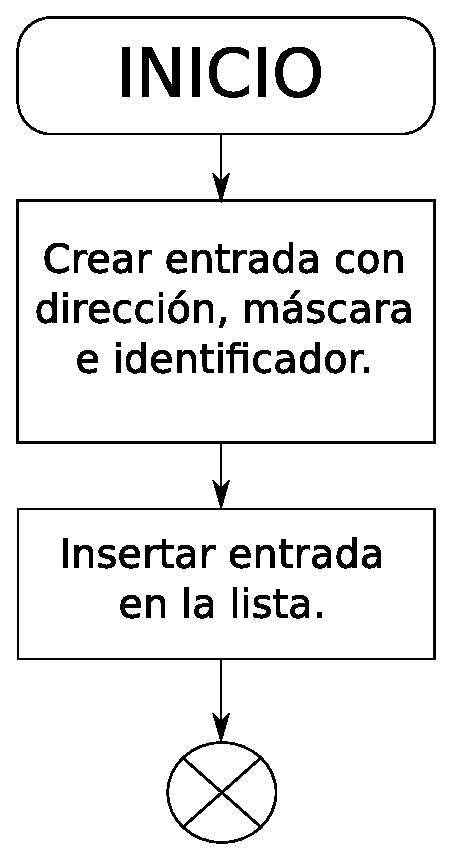
\includegraphics[scale=0.50]{4-implementacion/graf/lluinsert.eps}
  \caption{Diagrama de flujos para la inserción de nuevos valores en LLU}
  \label{fig:lluinsert}
\end{figure}

\subsubsection{Búsqueda}

Cuando la función encargada del lookup recibe una dirección IP de destino, realiza los siguientes pasos:

\begin{itemize}
	\item Coloca un iterador al comienzo de la lista, con el fin de comenzar el recorrido por la misma.
	\item Realiza un AND con el valor de máscara del nodo que está siendo apuntado. Si el resultado de la operación es igual al valor de dirección de red de dicho nodo, entonces se retorna con el valor identificador de decisión, ya que ese es el prefijo más largo según el orden establecido. En otro caso, continúa la búsqueda en el siguiente nodo.
\end{itemize}

Dichos pasos pueden verse graficados en la figura~\ref{fig:llusearch}

\begin{figure}[H]
  \centering
	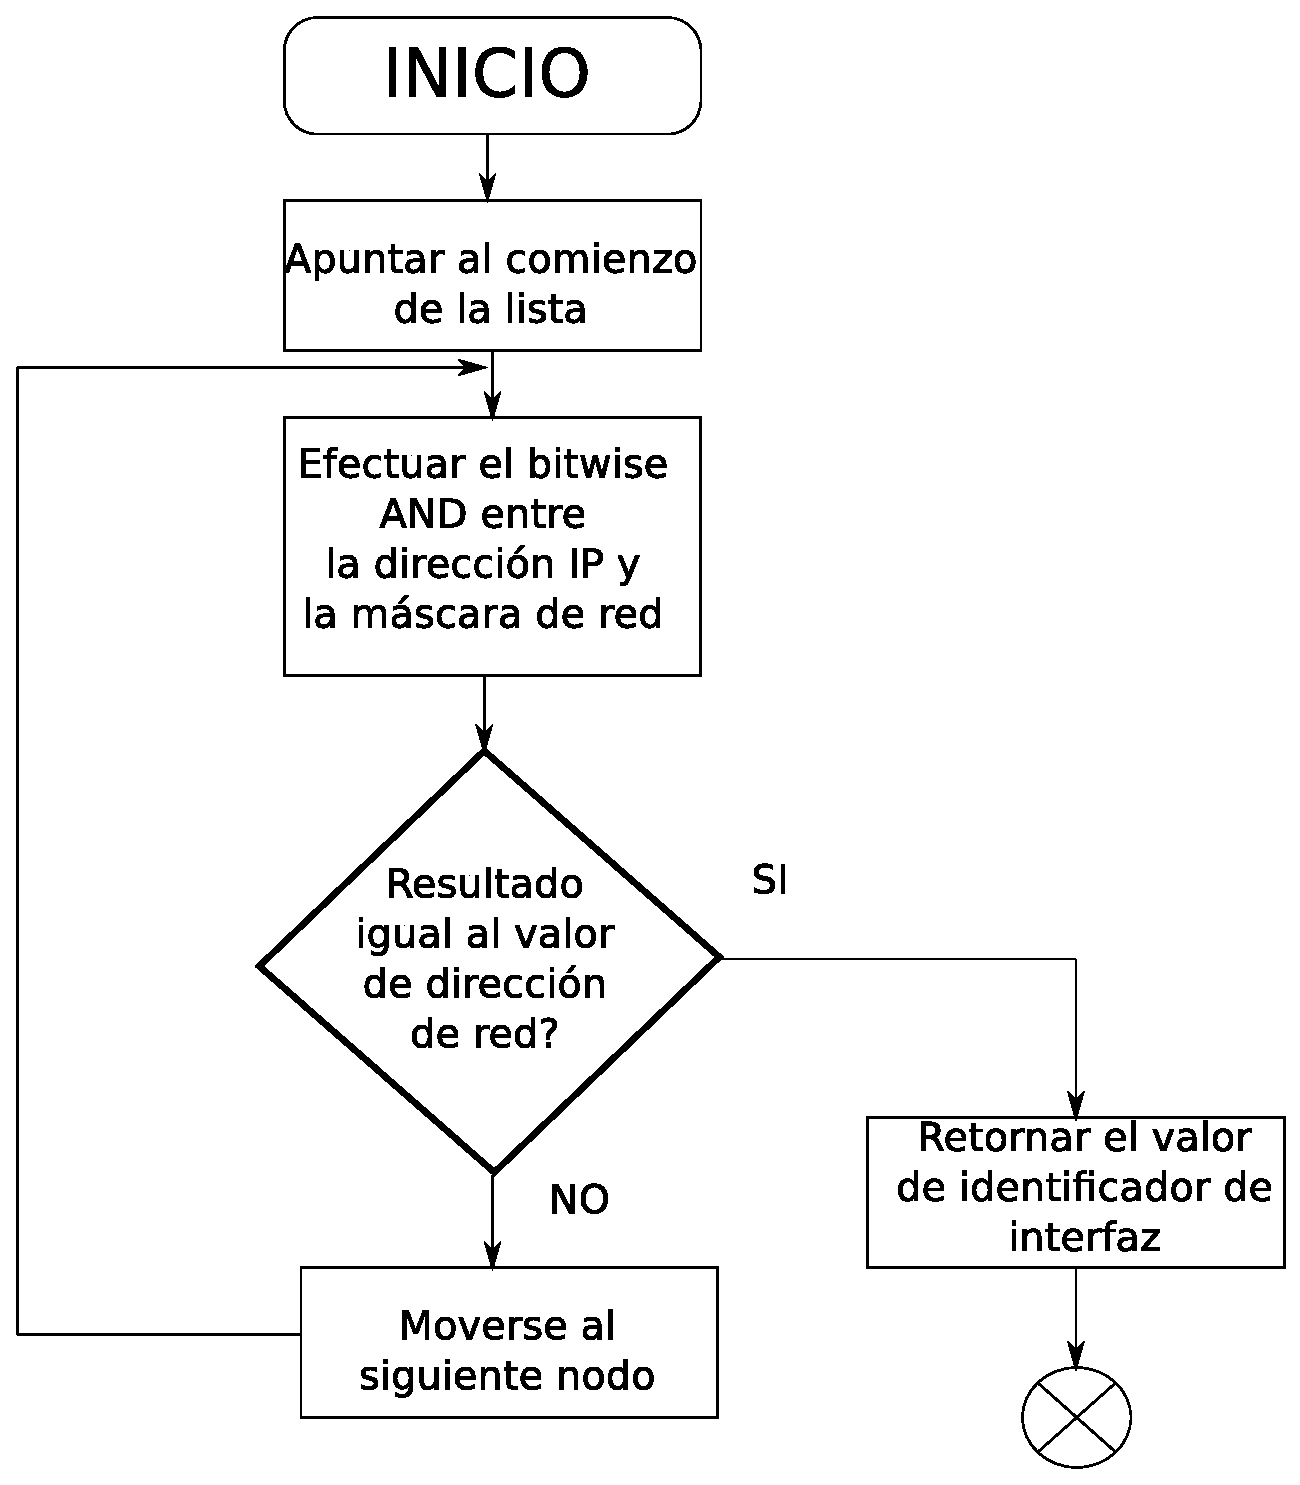
\includegraphics[scale=0.50]{4-implementacion/graf/llusearch.eps}
  \caption{Diagrama de flujos para la búsqueda LLU}
  \label{fig:llusearch}
\end{figure}

\subsection {Búsqueda en Árbol unibit}

Se implementaron 2 clases. 

\begin{itemize}
	\item \textit{trienode.h}: define las características de cada nodo del árbol.
	\item \textit{trie.h}: contiene el árbol unibit, como así también las funciones de búsqueda e inserción de nodos. También contiene una función para la creación de la tabla de ruteo de 100 valores.
\end{itemize}


En este contexto, pueden existir 2 tipos de nodo:

\begin{itemize}
	\item Común: no está asociado a una decisión. Es decir, sólo sirve como "nodo intermedio" en el recorrido por la estructura del árbol.
	\item Decisión: contiene un valor que identifica a la decisión a tomar. En este caso, la interfaz por donde se direcciona el paquete.
\end{itemize}

Cada nodo cuenta con los siguientes campos:
\begin{itemize}
	\item gw: es un identificador de la decisión a tomar. En los nodos no asociados a una decisión (nodos comunes), tiene el valor estipulado en la macro NONE.
    \item zero / one: son punteros a nodo, asociados a los valores de bit 0/1 del prefijo que se esté leyendo.

\end{itemize}

\subsubsection{Inserción de nuevas entradas}

La función de inserción toma como entrada una dirección y una máscara de red, así como también un valor de decisión asociado a la entrada en tabla. Lleva a cabo los siguientes pasos:
\begin{itemize}
	\item Partiendo con un puntero de recorrido desde el nodo raíz, el procedimiento se encuentra contenido en un bucle controlado por la longitud de la máscara de red. Es decir, en cada iteración se hace un testeo de bit de dicha máscara, comenzando por el bit más significativo. 
	\item Si éste es igual a uno, la iteración se lleva a cabo.
	\item En ella, se hace un testeo de bit, pero de la dirección de red.
	\item Si el mismo es igual a cero, se desplaza el puntero de recorrido hacia el nodo apuntado por \textit{zero}.
	\item En caso de no existir dicho nodo, se lo crea y recién entonces se desplaza el puntero de recorrido.
	\item Un procedimiento análogo se lleva a cabo en caso de que el testeo de bit sea igual a uno.
	\item Una vez finalizado el bucle, se escribe el valor de decisión en el nodo que esté siendo apuntado por el puntero de recorrido.
\end{itemize}

La inserción se ve representada en la figura~\ref{fig:utlinsertfc}

\begin{figure}[H]
  \centering
	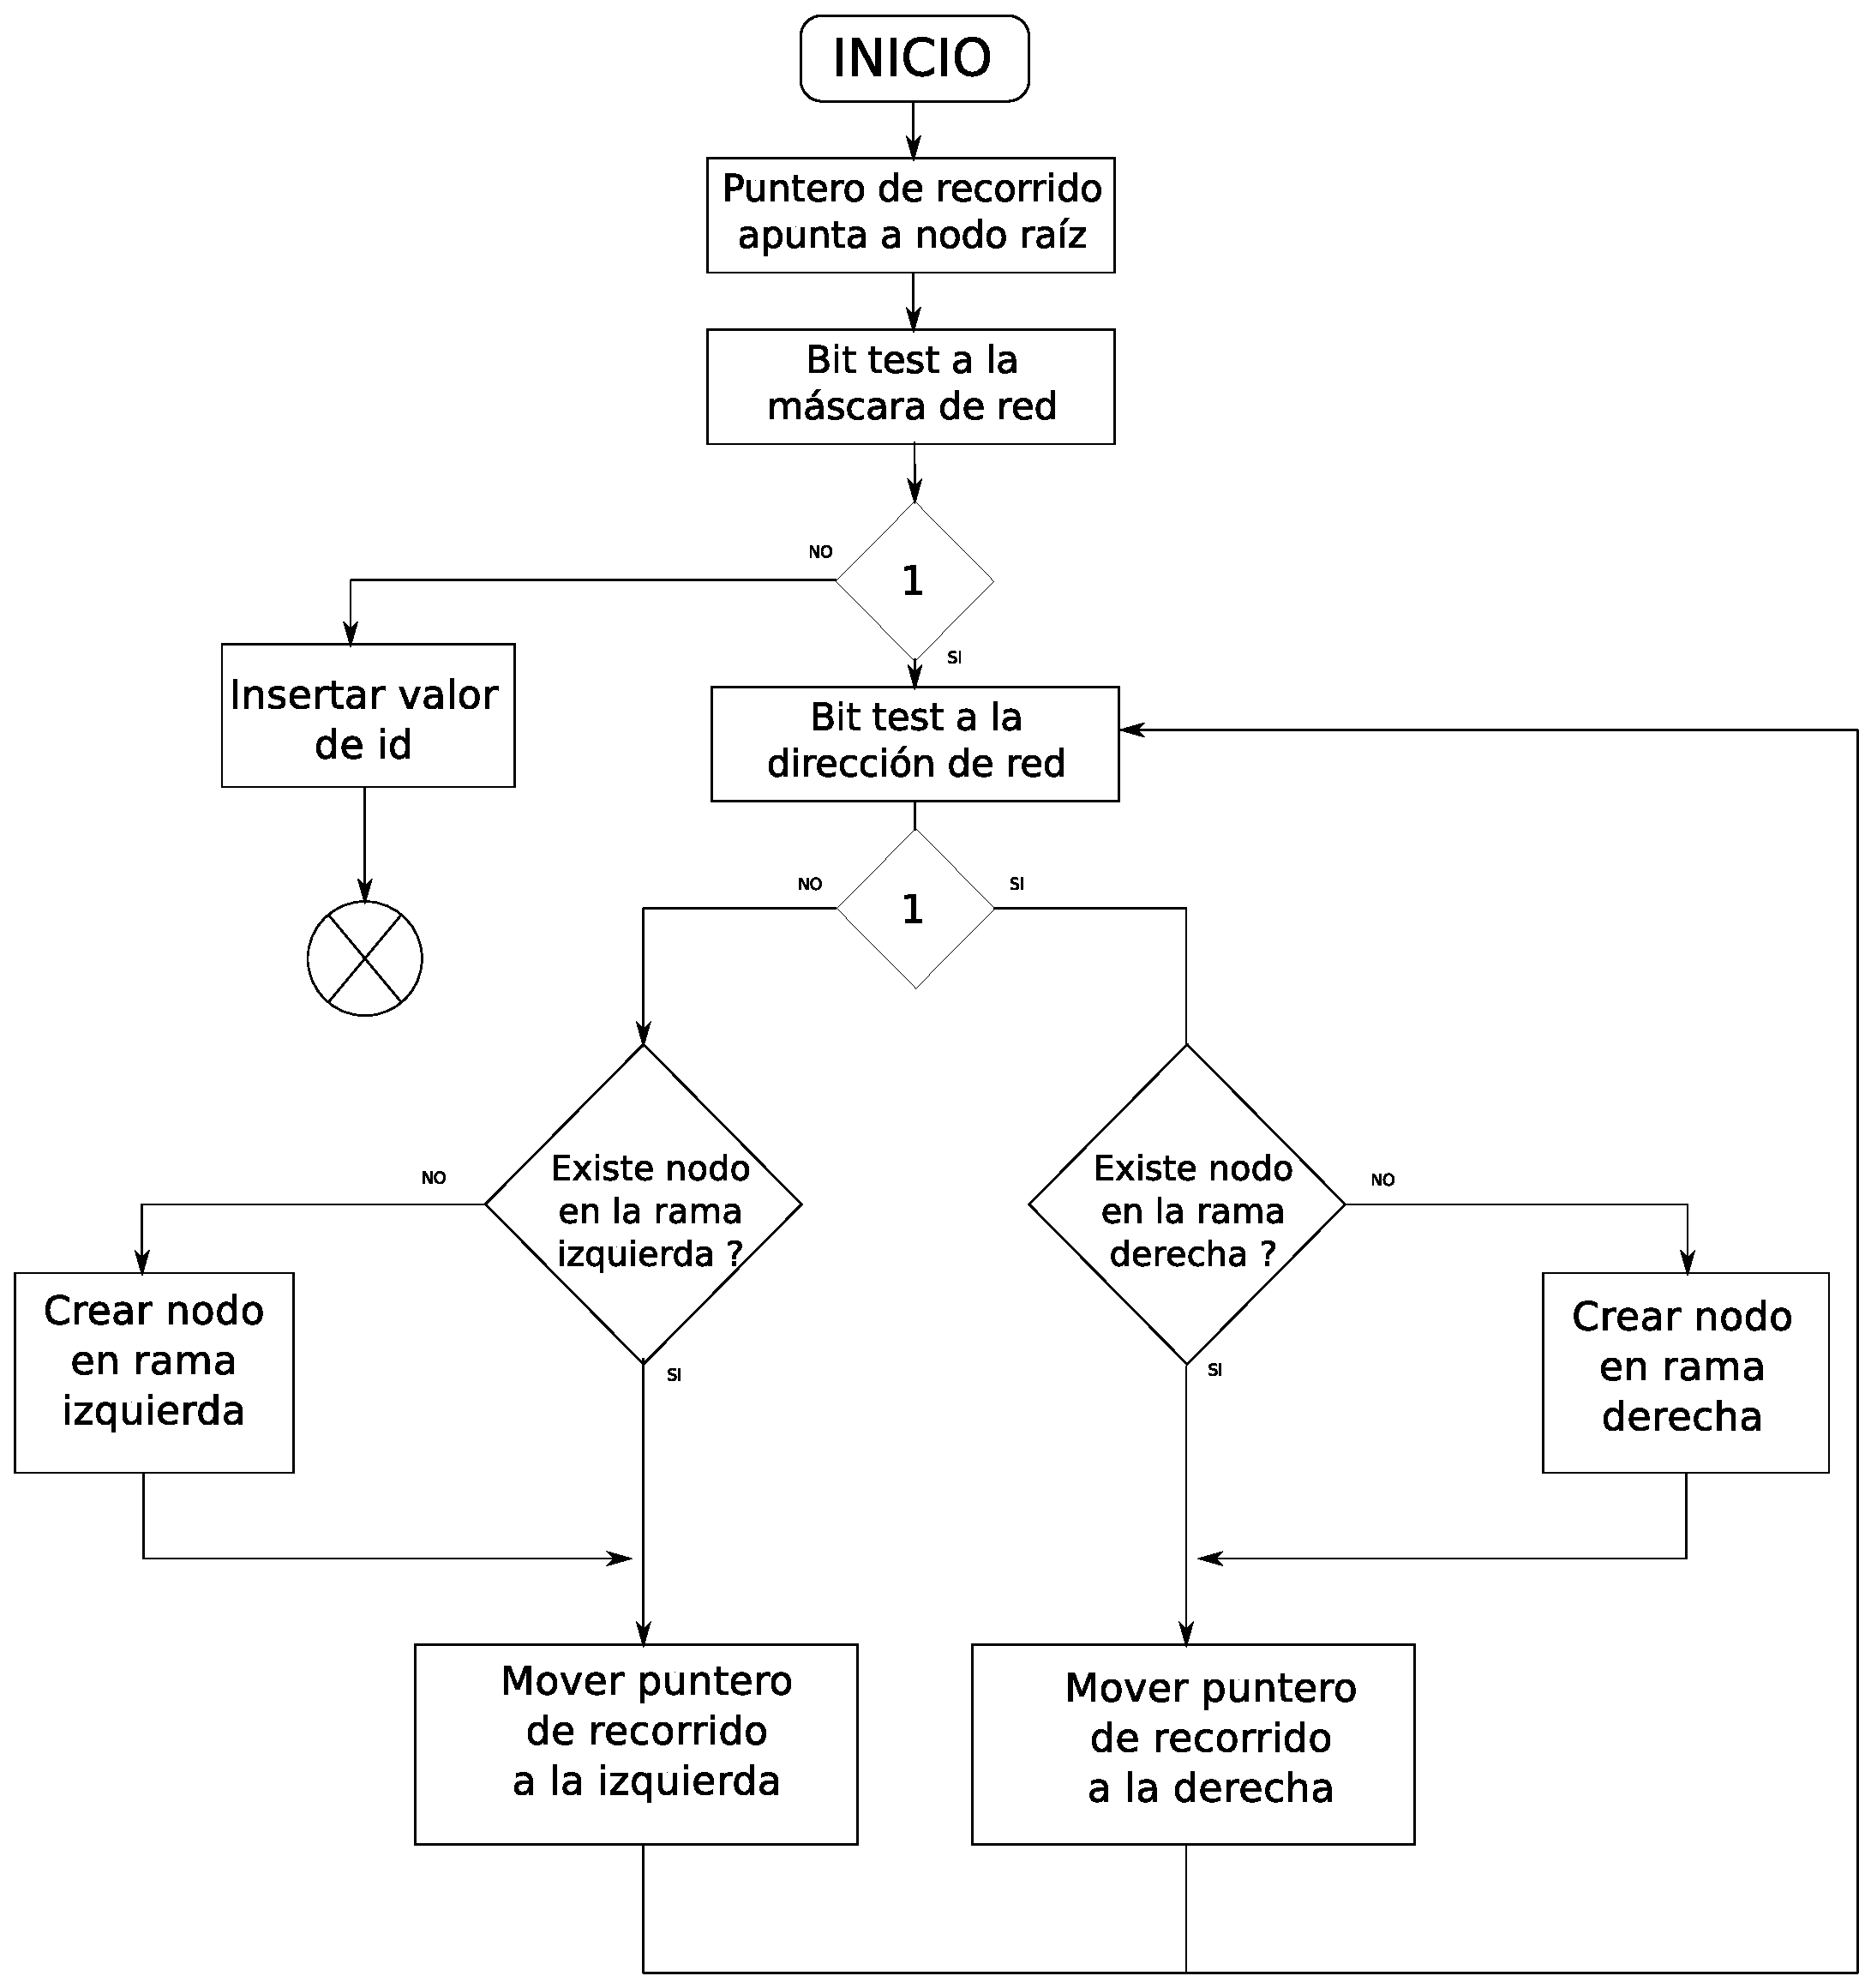
\includegraphics[scale=0.40]{4-implementacion/graf/utlinsert.eps}
  \caption{Diagrama de flujos para la inserción de valores en árbol unibit}
  \label{fig:utlinsertfc}
\end{figure}


\subsubsection{Búsqueda}

El algoritmo de búsqueda toma como entrada la dirección IP de destino del paquete a clasificar. Luego de ello realiza las siguientes acciones:
\begin{itemize}
	\item Hace un testeo bit a bit de dicha dirección, partiendo con un puntero de recorrido desde el nodo raíz.
	\item Si el bit de la dirección es 0 y el puntero zero está apuntando hacia algún nodo, el puntero de recorrido se mueve al nodo apuntado por el puntero zero.
	\item En caso contrario, se mueve al nodo apuntado por el puntero one (En caso de que exista alguno).
\end{itemize}

Esto se repite nodo a nodo, hasta que ocurre alguna de las siguientes situaciones:

\begin{itemize}
    	\item El puntero de recorrido queda varado en un nodo decisión, con lo cual se retorna el valor de gw.
    	\item El puntero de recorrido queda varado en un nodo común. 
\end{itemize}


Contemplando esta última posibilidad, el algoritmo hace que en cada nodo se chequee si se trata de un nodo decisión. En dicho caso, se almacena el campo gw en una variable y se continua el recorrido. Si se da un caso en el cual el nodo de recorrido queda apuntando a un nodo común y luego de testear un bit se determina que el mismo no tiene un nodo asociado (es decir, que alguno de los punteros zero / one esté en NULL) la función retorna la variable anteriormente mencionada. 

Cabe mencionar también que la ruta por defecto se inserta en el nodo raíz del árbol.

El procedimiento de lookup se ve representado en la figura~\ref{fig:utlsearch}

\begin{figure}[H]
  \centering
	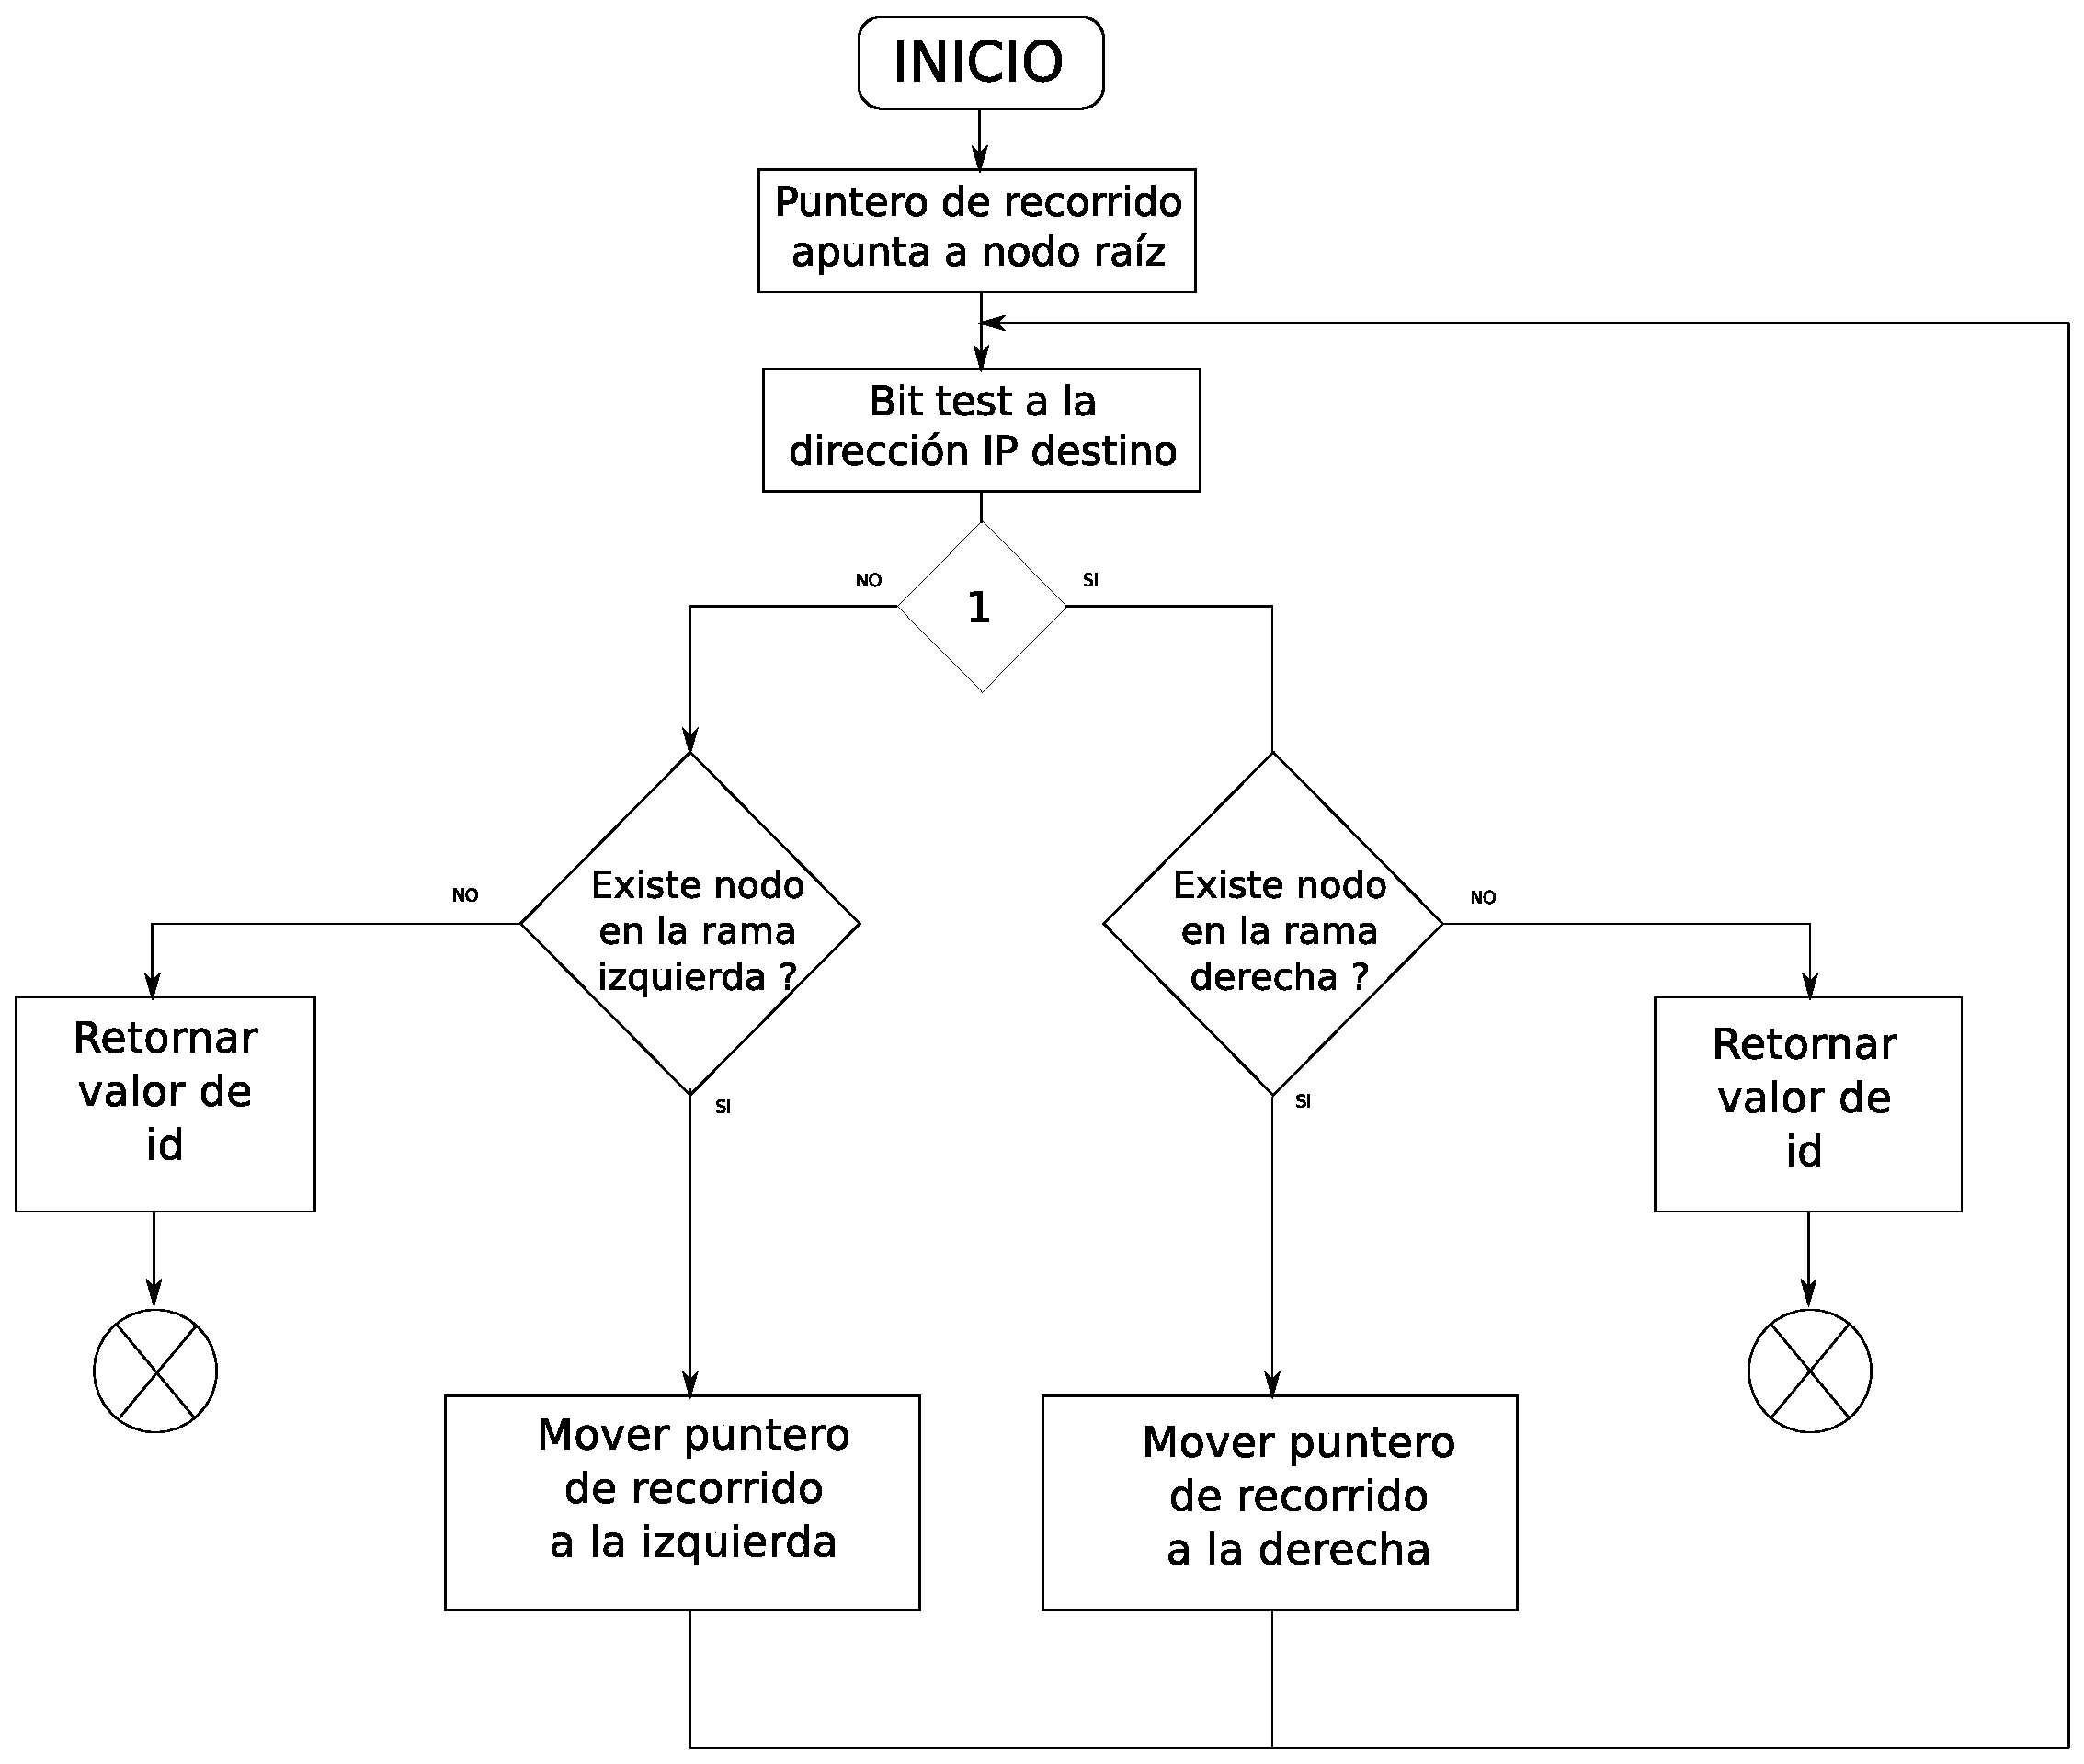
\includegraphics[scale=0.40]{4-implementacion/graf/utlsearch.eps}
  \caption{Diagrama de flujos para la búsqueda en árbol unibit}
  \label{fig:utlsearch}
\end{figure}

\begin{figure}[H]
  \centering
	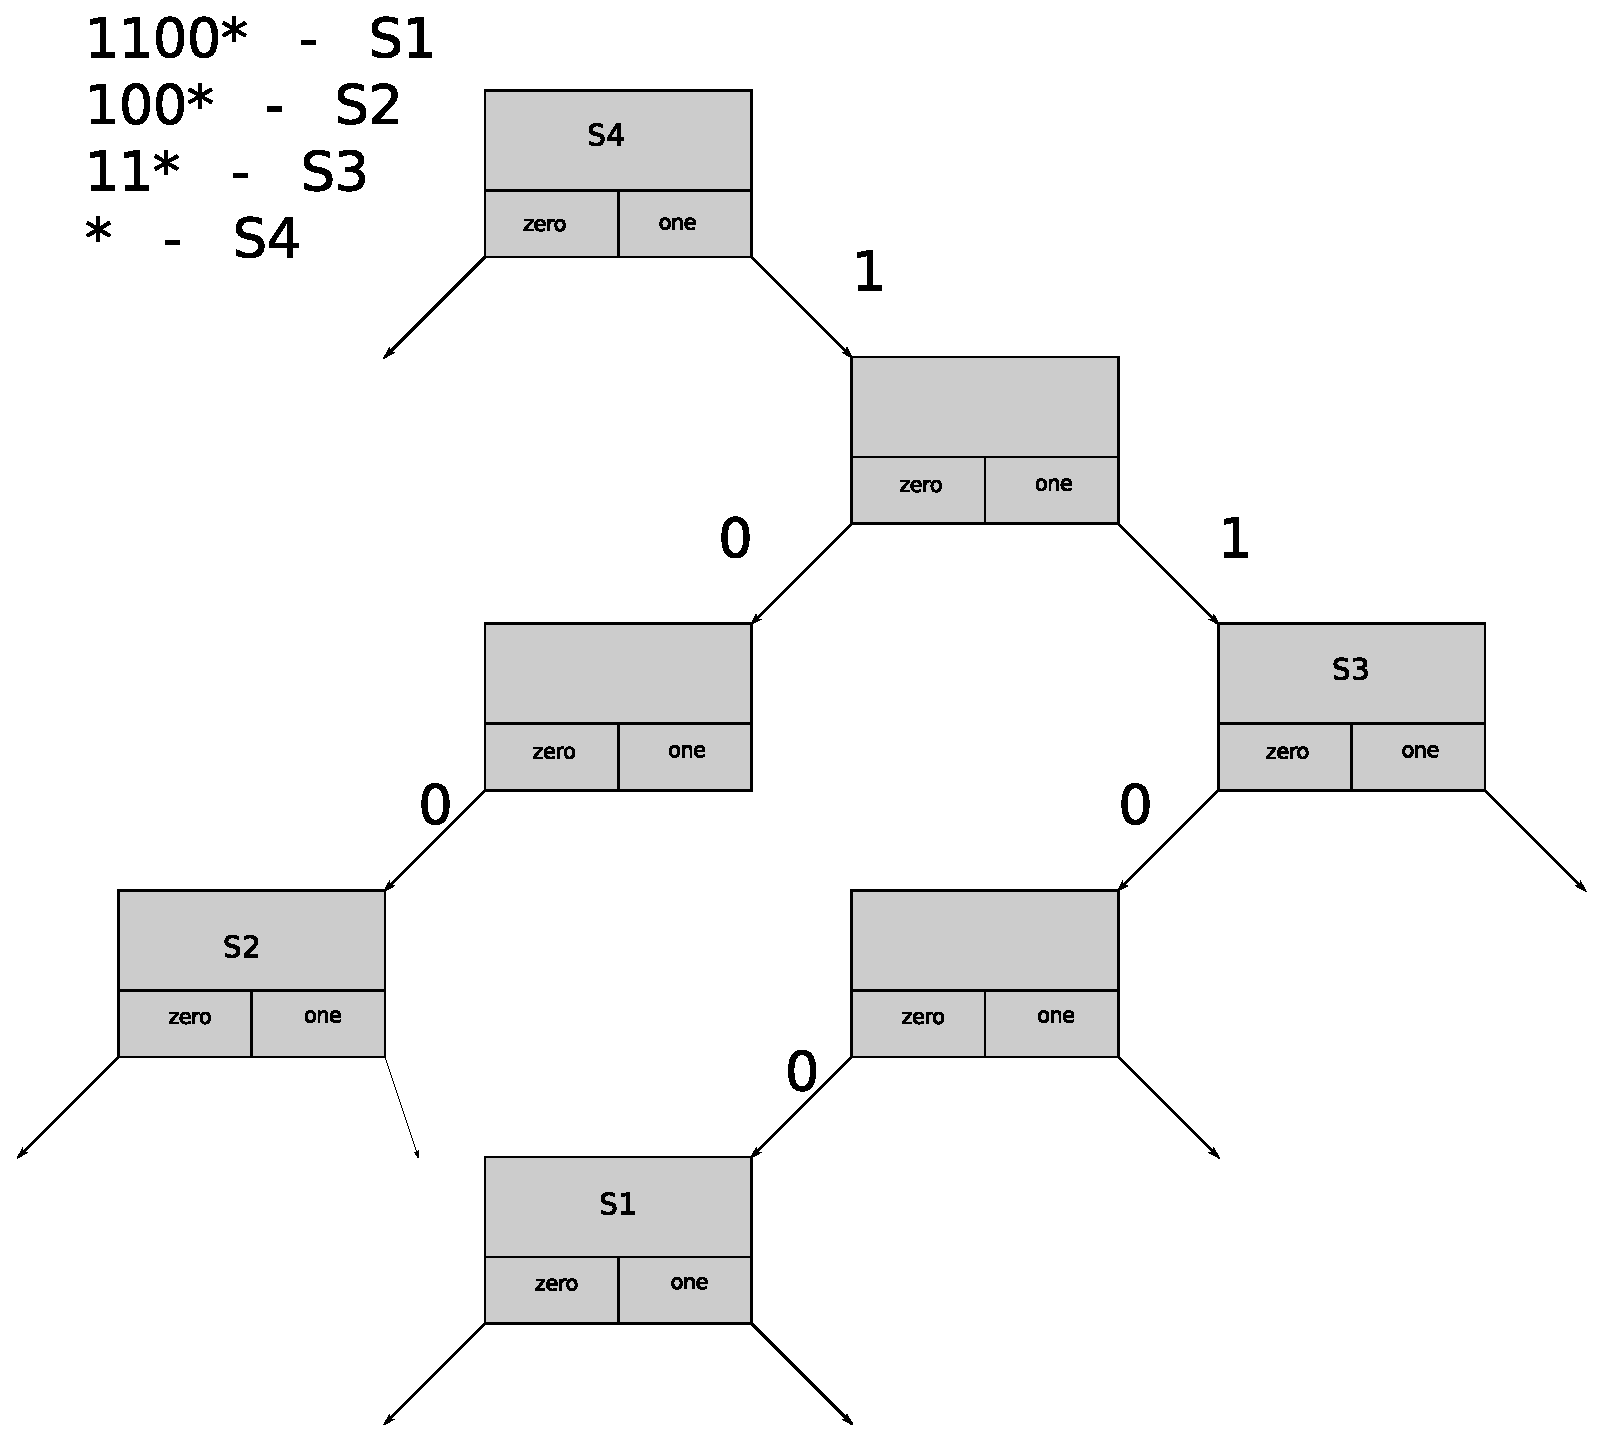
\includegraphics[scale=0.50]{4-implementacion/graf/lluinsert09.eps}
  \caption{Ejemplo de inserción de prefijos en árbol unibit}
  \label{fig:lluinsert}
\end{figure}

En la figura ~\ref{fig:lluinsert} se encuentra ejemplificada la inserción de 3 prefijos más la ruta por defecto. 

Comenzando por el nodo raíz, se inserta el prefijo 1100*. Para ello es necesaria la creación de 4 nodos hijos, uno por cada bit del prefijo. 

A continuación es insertado el prefijo 100*. Para el primer bit ya se encuentra creado el nodo, por lo cual se crean los 2 restantes necesarios.

Luego se inserta el prefijo 11*. Como anteriormente se había insertado el 1100* los nodos necesarios ya existen, por lo cual la inserción es trivial.

Por último en el nodo raíz se inserta la ruta por defecto (S4 en este ejemplo).

Tomando como ejemplo alguna dirección IP que comienza con 1100, puede verse que la búsqueda tomará el camino \textit{Raíz - one - one - zero - zero} y culminará en el nodo cuyo identificador de decisión es S1. 

Vale la pena considerar qué sucede si la dirección IP comienza con 1101. En este caso el camino que seguirá la búsqueda es \textit{Raíz - one - one - zero} y el puntero de recorrido quedará varado allí, ya que no existe en dicho punto un nodo asociado al puntero one. Recuérdese que en cada iteración, el algoritmo de búsqueda chequea si el nodo apuntado por el puntero de recorrido es decisión. Para este caso puede verse que en la segunda iteración (cuando se ha recorrido \textit{Raíz - one - one}) el algoritmo se encuentra parado en un nodo decisión y por lo tanto almacena el valor contenido en dicho nodo (S3) y procede a continuar. Cuando se encuentre varado en el próximo, lo que hará es retornar con el valor mencionado anteriormente. 

\subsection {Cache}

Se implementó una cache directa que consta de una tabla hash de 16 entradas, aunque este tamaño puede ser modificado mediante la macro CACHE\_SIZE. Las colisiones se resuelven por reemplazo directo. La misma fue testeada con ambos algoritmos mencionados anteriormente. Para ello, se agregó una lógica adicional que consistió en:

\begin{itemize}
	\item Al tomar una dirección IP, chequear primero si el valor de decisión se encuentra en caché.
	\item Si está, retornar dicho valor.
	\item En otro caso, efectuar el lookup y almacenar el valor de decisión en caché. Para dicho almacenamiento, se efectúa un hash en la dirección IP, que consiste en calcular el resto de la división entre dicha dirección y el valor de CACHE\_SIZE. El resultado es utilizado como índice para el almacenamiento en la tabla.
\end{itemize}

Para evitar el overhead introducido por el uso de clases, se optó por una implementación basada en una estructura, a la cual se denominó \textit{HashEntry}. La misma cuenta con los siguientes campos:

\begin{itemize}
	\item address: Dirección IP almacenada.
	\item gw: Identificador de decisión.
	\item empty: Indica si la entrada de tabla está vacía.
\end{itemize}

\section{Rutina de servicio de interrupción (Interrupt service routine, ISR)}

Como se mencionó anteriormente, el módulo Uplink envía interrupciones al procesador. A fin de poder procesarlas en el software se implementó una ISR (Interrupt Service Routine) que hace uso de 3 elementos principales:

\begin{itemize}
	\item \textit{store\_array}: Es un buffer en el cual se van almacenando las palabras enviadas por el módulo Uplink.
	\item \textit{i}: Es un subíndice que sirve para moverse dentro del buffer anteriormente mencionado.
	\item \textit{flag}: Es un indicador que se incrementa cada vez que se produce una interrupción.
\end{itemize}

\textit{store\_array} está implementado como una matriz de enteros, y tiene 3 columnas. De esta manera, cada fila cuenta con con 96 bits de los cuales se utilizan 72 de ellos para almacenar las palabras enviadas por Uplink.

Cada vez que el procesador recibe una interrupción, lleva a cabo la lectura del valor recibido y la almacena en \textit{store\_array}, en el lugar indicado por \textit{i}. Luego el subíndice se incrementa, al igual que \textit{flag}.

En la función principal (main) existe una variable llamada \textit{flag2}. A ésta se le asigna el valor de \textit{flag}. Al producirse una interrupción, el valor de \textit{flag} se modifica y por lo tanto la condición de igualdad entre \textit{flag} y \textit{flag2} ya no se cumple. En ese momento se utilizan los valores almacenados en \textit{store\_array} para llevar a cabo el algoritmo de clasificación. Dichos valores a utilizar dependerán de la versión de Uplink que se esté utilizando:

\begin{itemize}
	\item Para la versión que envía quince palabras de 32 bits, es necesario esperar a la quinta palabra de 96 bits en \textit{store\_array} para poder localizar la dirección IP de destino, necesaria para realizar la clasificación. En la figura ~\ref{fig:ip15pal} se muestra cómo está localizada dicha dirección. 
	\item Para la versión que envía sólo una palabra de 32 bits, el procedimiento es trivial ya que esa misma palabra es la dirección IP de destino.
\end{itemize}


Una vez llevado a cabo el procedimiento de clasificación, \textit{flag2} se iguala de nuevo al valor de \textit{flag }y el proceso se repite.


\begin{figure}[H]
  \centering
	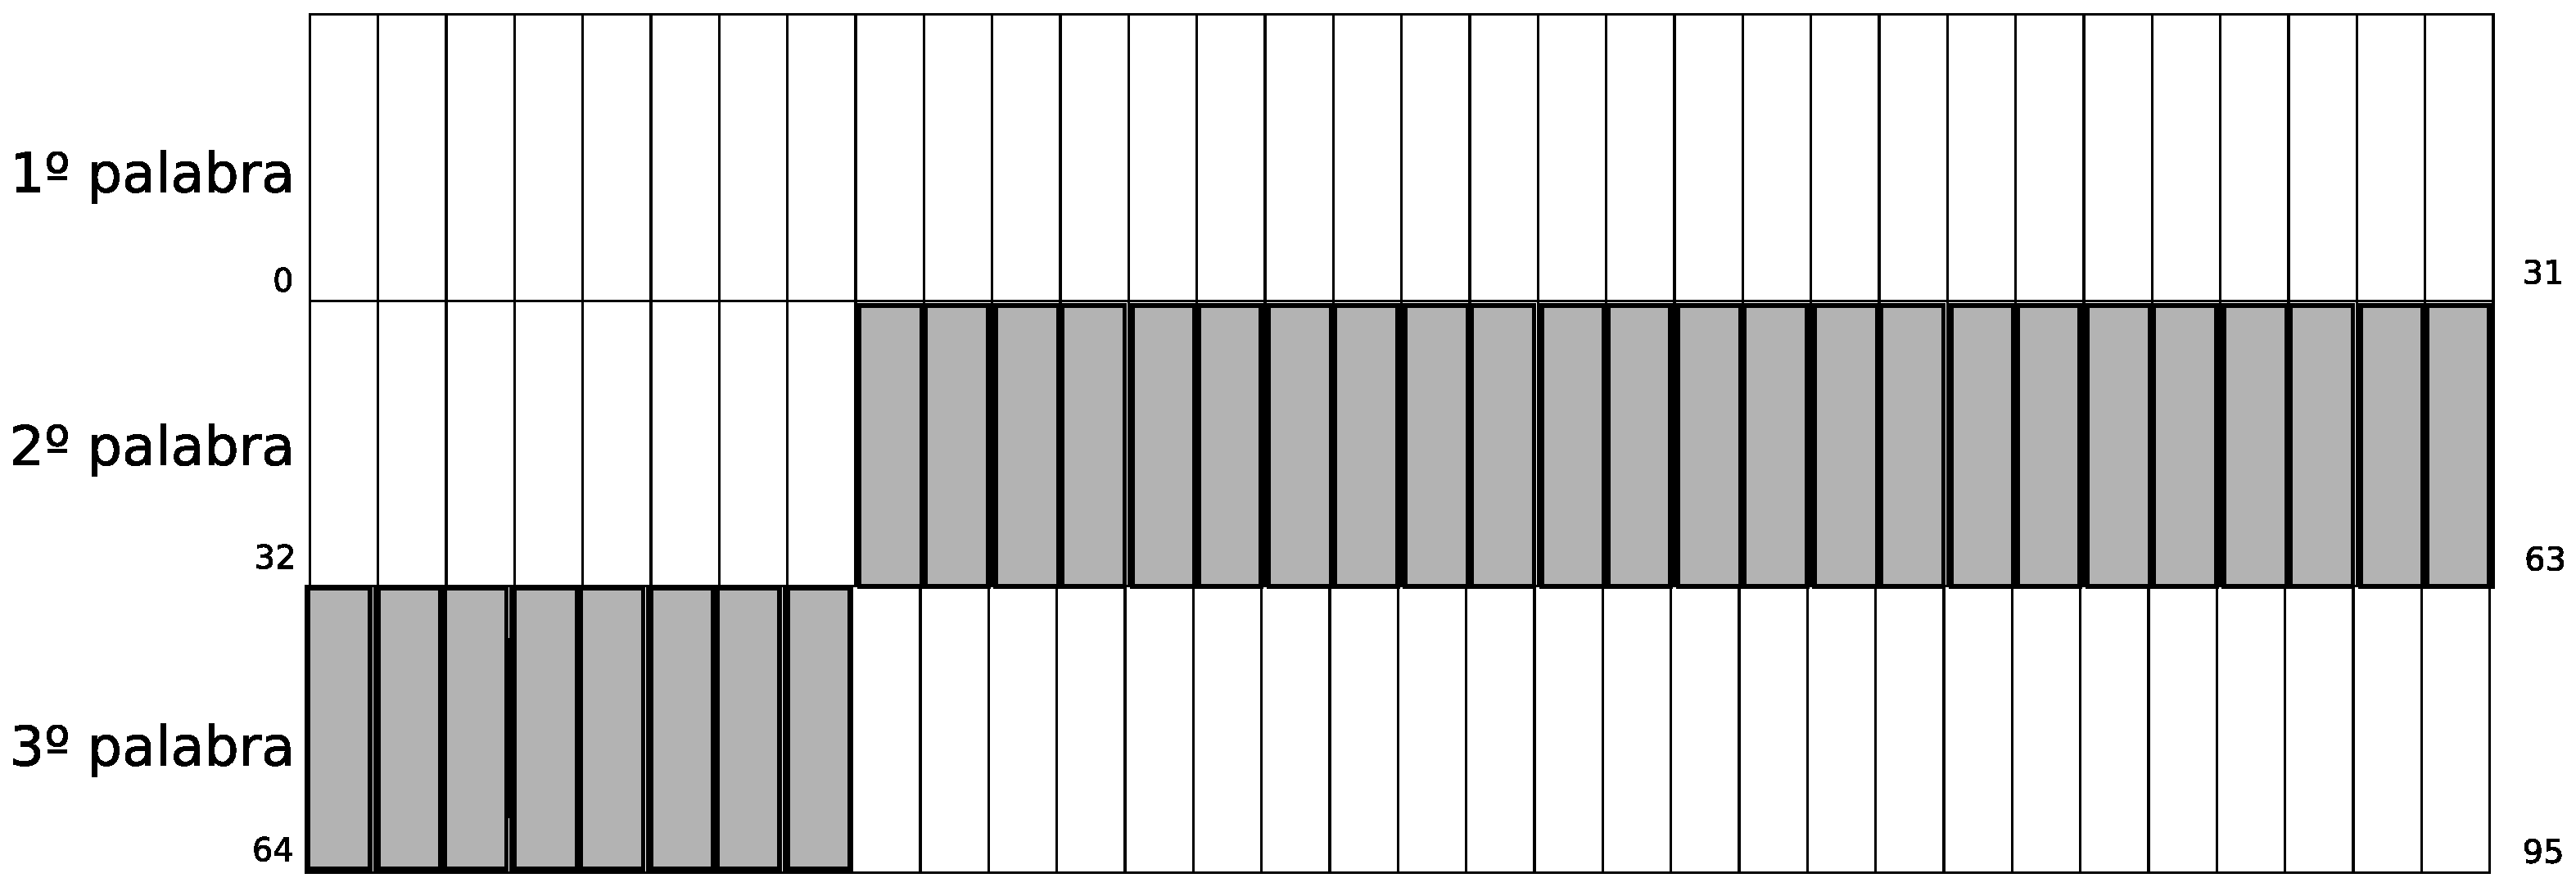
\includegraphics[scale=0.30]{4-implementacion/graf/ip15pal.eps}
  \caption{Ubicación de la dirección IP dentro de una palabra de 96 bits en store\_array, para la versión de Uplink que envía 15 palabras de 32 bits}
  \label{fig:ip15pal}
\end{figure}

\chapter{Integración}
\section{Plataforma}

El hardware utilizado fue la placa de desarrollo Altera DE2, cuyas características principales son:

\begin{itemize}
	\item FPGA: Cyclone II EP2C35F672C6
	\item USB Blaster integrado, para configuración de FPGA
	\item Memoria: 8 MB SDRAM, 512 KB SRAM, 4 MB Flash
	\item Clock de 50 MHz
\end{itemize}

Para una descripción más detallada, referirse al Apéndice A. A su vez, la FPGA incluida en esta placa cuenta con las siguientes características:

\begin{itemize}
	\item Elementos lógicos: 33216
	\item Bit totales de RAM: 483840
	\item Multiplicadores embebidos: 35
	\item PLLs: 4
	\item Cantidad máxima de pines definidos por el usuario: 475
\end{itemize}


\subsection{Microprocesador NIOS II}
El Nios II es un procesador RISC de 32 bits de propósito general que cuenta con las siguientes especificaciones:
\begin{itemize}
	\item Set de instrucciones, bus de datos y espacio de direcciones de 32 bits. 32 registros de propósito general y soporte de hasta 32 interrupciones.
	\item Acceso a una variedad de periféricos e interfaces a memorias y periféricos fuera del chip.
	\item Unidad de manejo de memoria (MMU) opcional para soportar sistemas operativos mas complejos.
	\item Unidad de protección de memoria (MPU) opcional.
	\item Entorno de desarrollo de software basado en GNU C/C++ integrado a Eclipse.
\end{itemize}

Para poder ser implementado en una mayor variedad de dispositivos el Nios II ofrece 3 configuraciones diferentes:  Nios II/f (fast), Nios II/s (Standard), and Nios II/e (Economy).

\subsubsection{Nios II/e}
El Core Nios II/e está diseñado para utilizar la menor cantidad de espacio posible. Esto es apropiado para FPGAs de bajo costo. El mismo Tiene las siguientes características:
\begin{itemize}
	\item Espacio de direcciones de hasta 2GB
	\item Gratuito, no requiere licencia 
\end{itemize}

\subsubsection{Nios II/s}
El Nios II/s está diseñado para mantener un balance entre rendimiento y costo. Entre sus características principales están:

\begin{itemize}
	\item Cache de instrucciones
	\item Espacio de direcciones de hasta 2GB
	\item Pipeline de 5 etapas
	\item Predictor de saltos estático
	\item Multiplicador y divisor por hardware. 
\end{itemize}

\subsubsection{Nios II/f}
El core Nios II/f está diseñado para ofrecer la mayor performance a expensas de un mayor tamaño, medido en unidades lógicas. Este core tiene las siguientes características:

\begin{itemize}
	\item Cache de instrucciones y de datos separadas
	\item MMU y MPU opcionales
	\item Espacio de direcciones de hasta 2GB
	\item Pipeline de 6 etapas
	\item Multiplicador por hardware en un ciclo
	\item Divisor por hardware opcional
	\item Predictor de saltos dinámico
\end{itemize}

En vista de que este último ofrece la mayor flexibilidad y el hardware seleccionado cuenta con las caracteristicas necesarias para soportarlo, sera el utilizado para esta implementacion. 




\subsection{Sintesis y Uso de Recursos}

En la figura \ref{fig:comple} es posible observar un diagrama completo del SoC que se implemento para este proyecto integrador.

\begin{figure}[H]
  \centering
	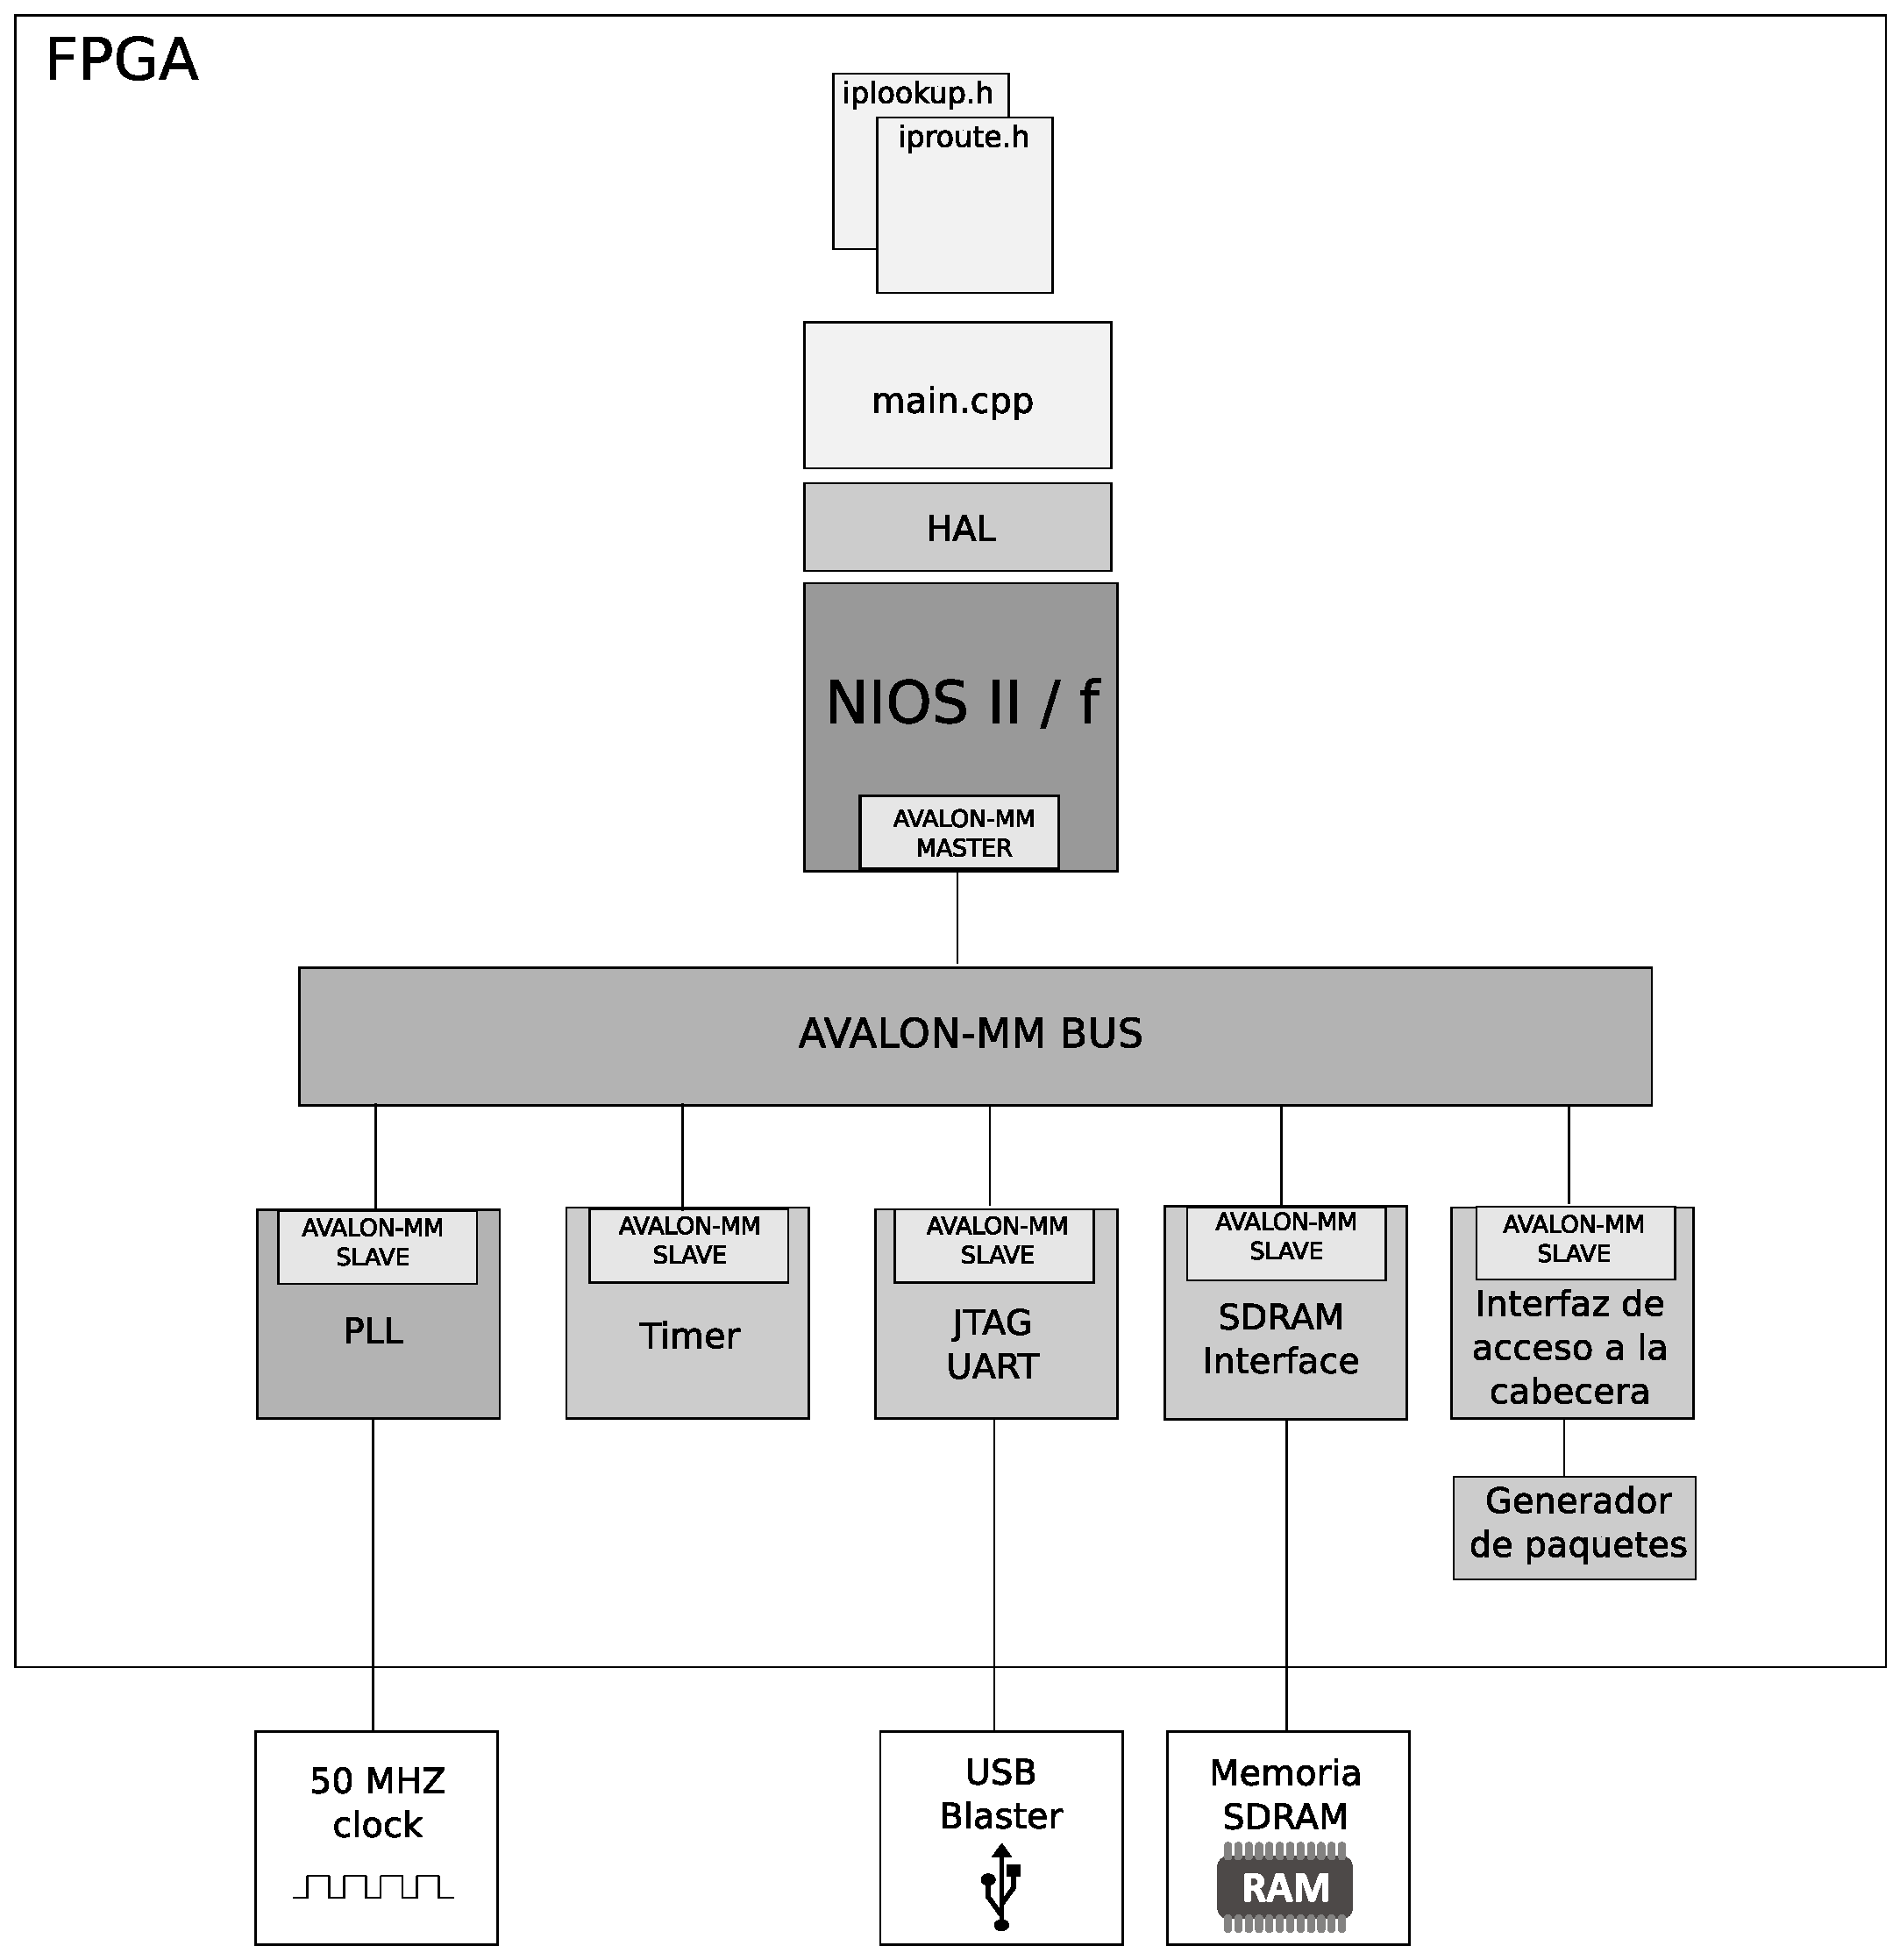
\includegraphics[scale=0.40]{4-implementacion/graf/sistema.eps}
  \caption{Esquematico completo del sistema embebido}
  \label{fig:comple}
\end{figure}

Los recursos totales utilizados por el proyecto completo fueron:
\begin{itemize}
\item Elementos lógicos: 4983
	\item Bits de RAM: 280627
	\item Multiplicadores embebidos: 2
	\item PLLs: 1
	\item Cantidad máxima de pines definidos por el usuario: 86
\end{itemize}

\begin{figure}[H]
  \centering
	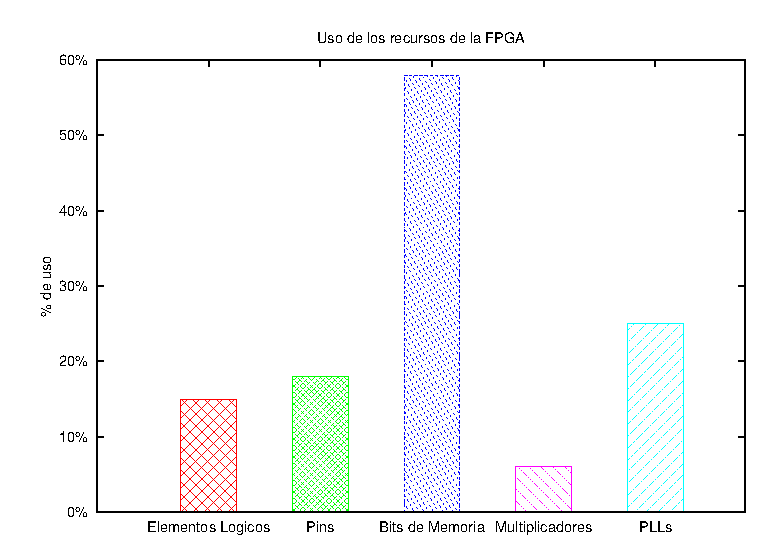
\includegraphics[scale=0.70]{4-implementacion/graf/fpga.eps}
  \caption{Uso de los recursos de la FPGA}
  \label{fig:fpga}
\end{figure}


\section{Verificación}
Se muestran a continuación varios casos de prueba que se realizaron para verificar el correcto funcionamiento del sistema.
\begin{table}
	\begin{tabular}{|>{\columncolor[gray]{0.8}}l|p{11cm}|} \hline
\multicolumn{2}{|>{\columncolor[gray]{0.8}}l|}{\textbf{Caso de Prueba: Funcionalidad del SoC}}\\ \hline
Propósito  & 1) Verificar la funcionalidad completa de System on Chip. 

2) Probar la correcta ejecución de software en el Nios II.

3) Comprobar el funcionamiento de las E/S del procesador. 
\\ \hline
 Prerrequisitos  & Se debe haber sintetizado el sistema completo y compilado sin errores el software. La placa debe estar conectada a la PC por USB mediante el cable correspondiente. \\ \hline
 Datos de Prueba & Se preparara un sistema básico que incluye un Nios II/f, la interfaz de memoria y un PIO conectado a los LEDs de la placa.

Se usa un Software en lenguaje C que va incrementando e imprimiendo en consola un valor entero mientras envía este valor, en binario, al PIO y por extensión a los LEDs.  \\ \hline
 Pasos & 1) Programar la FPGA con el sistema completo.

2) Descargar el software al Microprocesador.

3) Iniciar la consola del NIOS II en la PC.\\ \hline
 Resultados Esperados & El valor del contador que se imprime por consola debe coincidir con el valor mostrado por los LED.\\ \hline
 Evaluación de la Prueba  & El resultado de la ejecución fue exitoso. \\ \hline
	\end{tabular}
	\caption{Caso de Prueba: Funcionalidad del SoC}
	\label{tab:testsoc}
\end{table}
\begin{table}
	\begin{tabular}{|>{\columncolor[gray]{0.8}}l|p{11cm}|} \hline
\multicolumn{2}{|>{\columncolor[gray]{0.8}}l|}{\textbf{Caso de Prueba: Interrupción, Envío y Recepción de datos}}\\ \hline
Propósito  & 1) Comprobar mediante un Custom Component (Apéndice D)  simple el funcionamiento de las interrupciones.

2) Enviar y recibir un dato estático por el bus sin errores. 
\\ \hline
 Prerrequisitos  & Se debe contar con el SoC completo y funcional.\\ \hline
 Datos de Prueba & Se prepara un Componente propio simple que interrumpe, envía un dato y espera que el procesador le responda con el mismo dato. 

Se utiliza un software que cuente con la Rutina de Interrupción correspondiente y que cuando reciba un dato responda con el mismo de manera inmediata, además de imprimirlo por consola.
 \\ \hline
 Pasos & 1) Programar la FPGA con el sistema completo.

2) Descargar el Software al Microprocesador.

3) Iniciar la consola del NIOS II en la PC.
\\ \hline
 Resultados Esperados & En la consola debe aparecer repetidamente el valor que fue generado en el Hardware. \\ \hline
 Evaluación de la Prueba  & El resultado de la prueba fue exitoso.\\ \hline
	\end{tabular}
	\caption{Caso de Prueba: Interrupción, Envío y Recepción de datos}
	\label{tab:enviorecepcion}
\end{table}
\begin{table}
	\begin{tabular}{|>{\columncolor[gray]{0.8}}l|p{11cm}|} \hline
\multicolumn{2}{|>{\columncolor[gray]{0.8}}l|}{\textbf{Caso de Prueba: Integridad de paquetes }}\\ \hline
Propósito  & 1) Comprobar que la cabecera llega completa y sin errores al software. 

2) Verificar que el paquete sale del sistema completo.

3) Validar la correcta escritura del resultado en el tag Adjunto.

4) Comprobar que el paquete pasa sin errores por todo el sistema. 

5) Verificar que no se pierden paquetes por errores propios del sistema. 
\\ \hline
 Prerrequisitos  & Se debe contar con la interfaz de acceso a la cabecera, el generador y el software necesario, completos y funcionales, y se debe conectar la salida de Write Output a los LEDs de la placa.\\ \hline
 Datos de Prueba & Se configura el generador para que la cantidad de ciclos de reloj entre paquetes sea la máxima (mínima tasa de datos). 

Se prepara el software para que lea la cabecera completa, imprima lo leído en consola y responda automáticamente con un resultado conocido. 
 \\ \hline
 Pasos & 1) Programar la FPGA con el sistema completo.

2) Descargar el Software al Microprocesador.

3) Iniciar la consola del NIOS II en la PC.
\\ \hline
 Resultados Esperados & En la consola debe aparecer impresa la cabecera del paquete tal cual los valores predefinidos y en los LEDs debe aparecer al final de cada paquete el número de paquete y el resultado conocido escrito.  \\ \hline
 Evaluación de la Prueba  & El resultado de la prueba fue exitoso.\\ \hline
	\end{tabular}
	\caption{Caso de Prueba: Integridad de paquetes}
	\label{tab:integridad}
\end{table}
\begin{table}
	\begin{tabular}{|>{\columncolor[gray]{0.8}}l|p{11cm}|} \hline
\multicolumn{2}{|>{\columncolor[gray]{0.8}}l|}{\textbf{Caso de Prueba: Funcionamiento de los algoritmos de clasificación }}\\ \hline
Propósito  & 1) Verificar que el lookup de direcciones se lleve a cabo según lo esperado.

\\ \hline
 Prerrequisitos  & Se debe contar con el software necesario para la clasificación de paquetes. Las pruebas se efectúan para cada algoritmo por separado. Se debe contar con un SoC que incluya un timer instanciado, que luego el software utilizara para medir los retardos en el acceso.
 \\ \hline
 Datos de Prueba & Se generan dentro del mismo software una tabla de ruteo y otra tabla que contendrá las direcciones para efectuar el test. 

Se prepara el software para que imprima los resultados en consola. 
 \\ \hline
 Pasos & 1) Programar la FPGA con el sistema completo.

2) Descargar el Software al Microprocesador. 

3) Iniciar la consola del NIOS II .
\\ \hline
 Resultados Esperados & En la consola debe aparecer la dirección leída y el identificador de decisión resultante para dicha dirección. \\ \hline
 Evaluación de la Prueba  & El resultado de la prueba fue exitoso.\\ \hline
	\end{tabular}
	\caption{Caso de Prueba: Funcionamiento del lookup.}
	\label{tab:retlook}
\end{table}


%\section{Distribucion Lineal}
 
\chapter{Resultados}

En este capítulo se presentan los datos obtenidos de la ejecución del proyecto bajo ciertas condiciones representativas, con la intención de validar la funcionalidad y también de encontrar los alcances y límites del mismo. Primero se estudia el tiempo de respuesta de los algoritmos de manera individual, a continuación el rendimiento en la configuración mas simple, luego el sistema completo bajo condiciones varias, y por ultimo se analiza la mejora introducida por el uso de la cache. Para la obtención de los datos que corresponden al sistema completo se utilizaron de manera complementaria scripts programados en lenguaje Python y en Bash. Durante todo el capítulo se usara LLU como acronimo de \textit{Linear Look Up} y UTL para referirse al \textit{Unibit Trie Lookup}. 


\section{Stress de software}

Con la intención de obtener un gráfico que represente el rendimiento de los dos algoritmos implementados, se mide el retardo de búsqueda en función de la posición de coincidencia en la tabla de enrutamiento. Se realizan las pruebas de manera independiente a la Interfaz de acceso a la cabecera con el fin de aisalar los efectos del mismo. En el eje de las abscisas se expresa la ubicación del prefijo mas largo en una tabla de 100 elementos  y en las ordenadas se puede observar el tiempo de búsqueda en ciclos de reloj.

\begin{figure}[h]
  \centering
	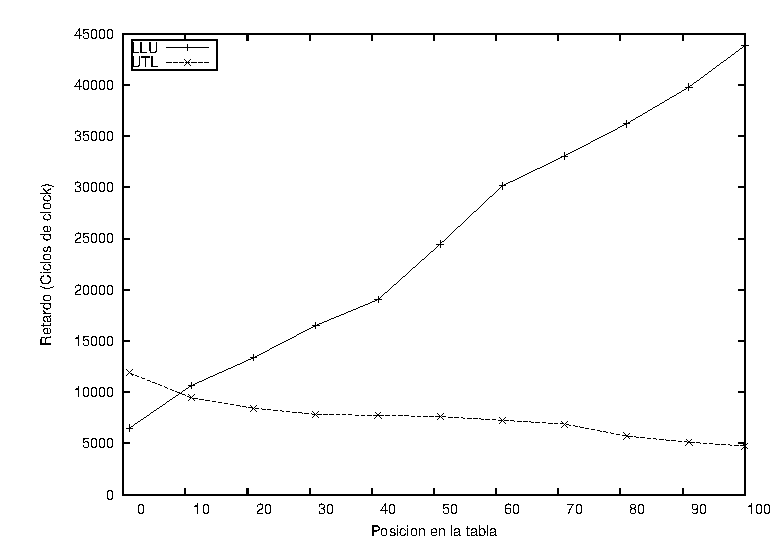
\includegraphics[width=0.8\textwidth]{5-resultados/graf/llu-utlsof.eps}
  \caption{Retardo de Búsqueda LLU vs UTL}
  \label{fig}
\end{figure}

\newpage
\section{Stress de hardware}
\begin{figure}[h]
  \centering
	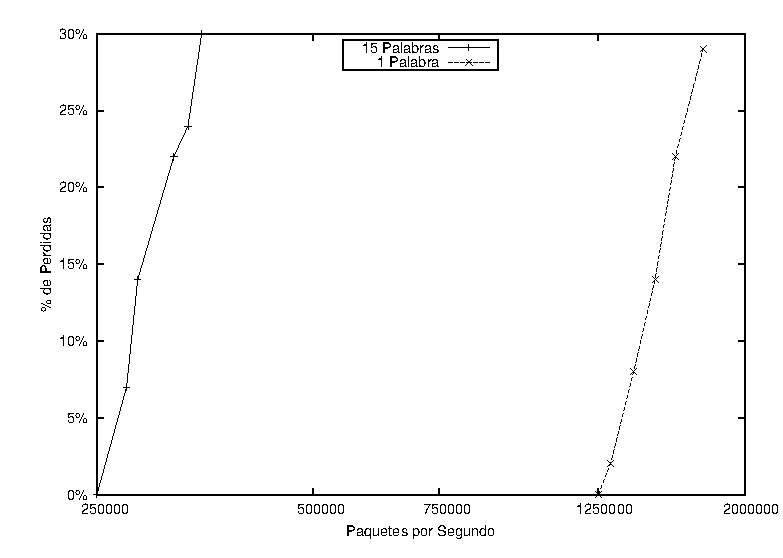
\includegraphics[width=0.70\textwidth]{5-resultados/graf/loop.eps}
  \caption{Caso Loopback para 1 y 15 palabras}
  \label{fig:loop}
\end{figure}
Se estudia en primer termino el caso loopback a los fines de encontrar los límites superiores del sistema determinado por la sección hardware. En este caso el software solo se limita a recibir los datos e inmediatamente después confirma el procesamiento, enviando un resultado predefinido de regreso al hardware. Se realizan las pruebas correspondientes para las dos versiones de Uplink.
En el eje de las abscisas de la figura \ref{fig:loop} es posible ver la cantidad de paquetes por segundo cuyo el origen corresponde a la mayor velocidad a la que es posible transmitir sin perdidas de datos. En las ordenadas se puede observar la cantidad de paquetes perdidos en valores porcentuales. Para obtener esta métrica se procesó una cantidad constante de paquetes, 9000, y luego se contrastó este valor con un contador global que el generador coloca en la ultima palabra de cada paquete. Así se calculó la cantidad paquetes perdidos, sobre la cantidad total de paquetes generados. Este mismo sistema es el usado en todos los gráficos posteriores.


\newpage
\section{Implementación Completa}

En este ensayo se verifica el rendimiento del sistema implementado de manera completa. Se considera tres puntos en las curvas que indican los tiempos de procesamiento de los algoritmos: un punto mínimo que corresponde al menor tiempo, un punto promedio que ejercita 10 entradas equidistantes a lo largo de la tabla y un punto máximo que indica el peor tiempo de acceso posible para un algoritmo dado. 

\subsubsection{a) Linear Lookup (LLU)}
Se evalúa el desempeño para los casos en lque se envian 1 y 5 palabras de 72 bits como ya se mencionó. Se observa que los valores de pérdida de paquetes para ambos casos difieren mucho para profundidades de busqueda pequeña (figura \ref{figminllu}), pero convergen a medida que la profundidad de busqueda aumenta (figuras \ref{figpromllu} y \ref{figmaxllu}). Este efecto era esperable ya que para accesos muy lentos a la tabla el retardo introducido por el hardware se vuelve despreciable.



\newpage
\begin{figure}[!h]
  \centering
	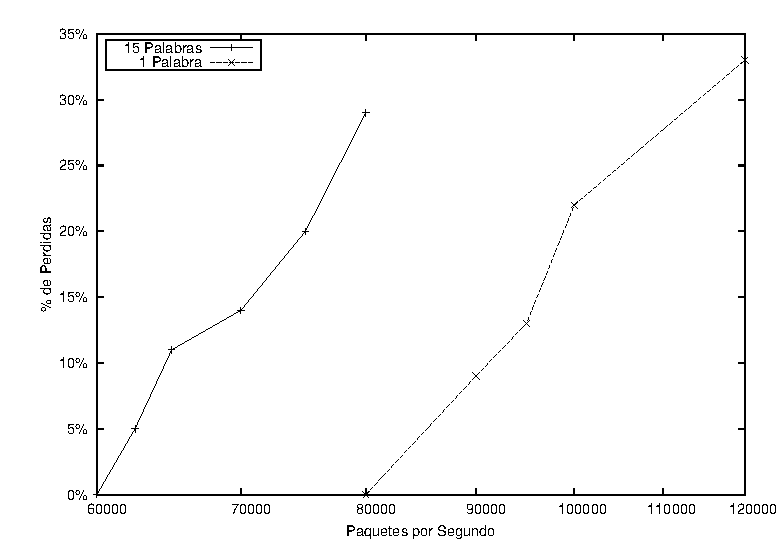
\includegraphics[width=0.7\textwidth]{5-resultados/graf/llumin.eps}
  \caption{Retardo mínimo LLU}
  \label{figminllu}
\end{figure}
\begin{figure}[!h]
  \centering
	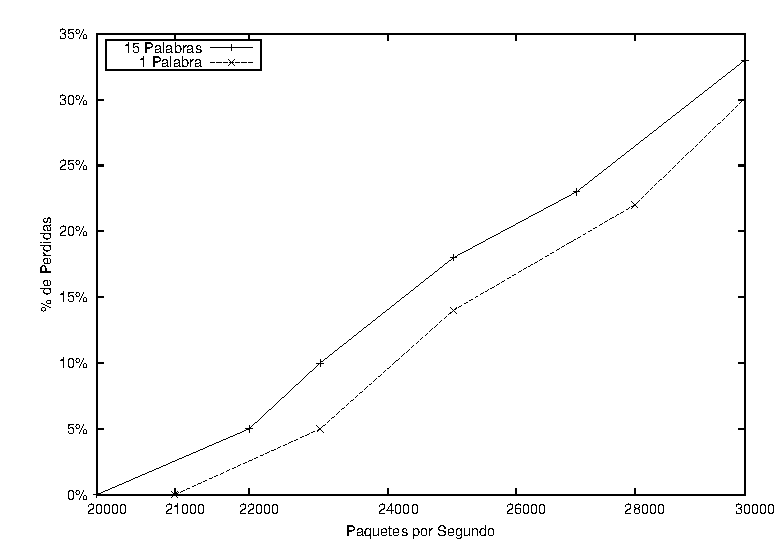
\includegraphics[width=0.7\textwidth]{5-resultados/graf/lluprom.eps}
  \caption{Retardo promedio LLU}
  \label{figpromllu}
\newpage
\end{figure}
\begin{figure}[!h]
  \centering
	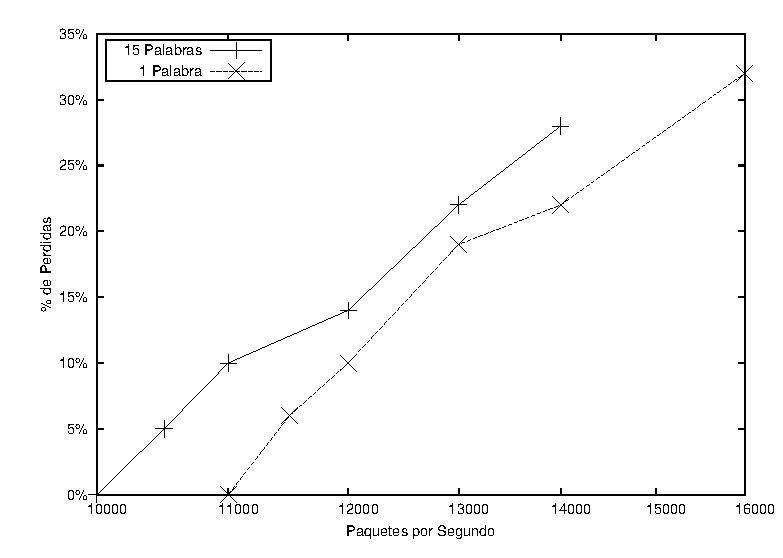
\includegraphics[width=0.7\textwidth]{5-resultados/graf/llumax.eps}
  \caption{Retardo máximo LLU}
  \label{figmaxllu}
\end{figure}



\newpage
\subsubsection{b) Unibit Trie Lookup (UTL) }

En los gráficos que corresponden al Unibit Trie Lookup es posible observar que existe una menor diferencia entre la máxima cantidad de paquetes que pueden ser transmitidos sin error en cada uno de los 3 puntos elegidos. También la diferencia entre enviar el paquete entero y solo la IP destino se reduce, lo que dá la pauta de que cuando el tiempo de acceso es uniforme el impacto de enviar 1 o 15 palabras tiende a ser menor.
\newpage
\begin{figure}[!h]
  \centering
	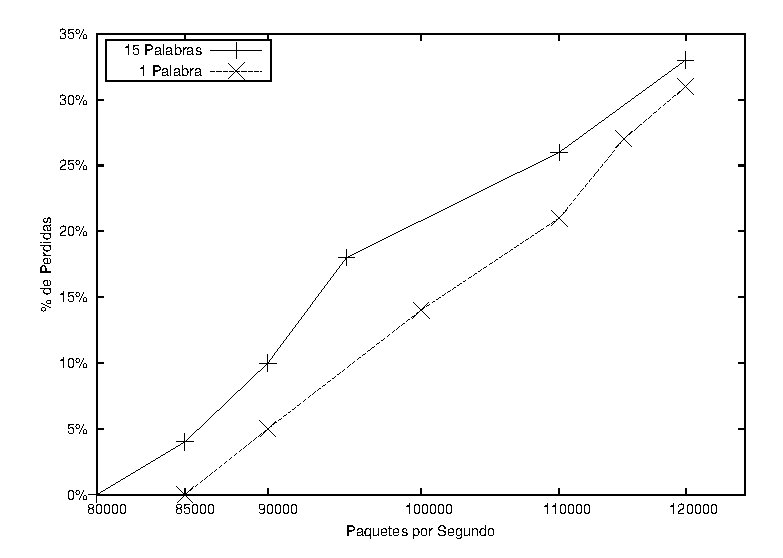
\includegraphics[width=0.7\textwidth]{5-resultados/graf/utlmin.eps}
  \caption{Retardo mínimo UTL}
  \label{fig}
\end{figure}
\begin{figure}[!h]
  \centering
	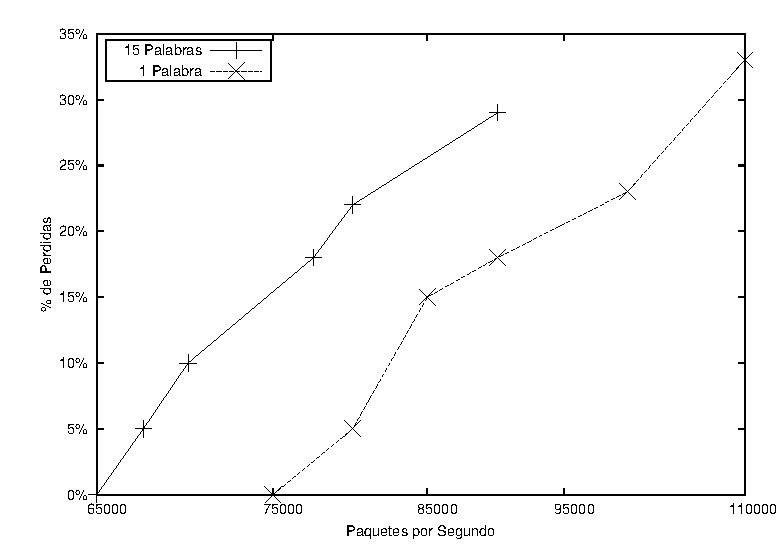
\includegraphics[width=0.7\textwidth]{5-resultados/graf/utlprom.eps}
  \caption{Retardo promedio UTL}
  \label{fig}
\end{figure}
\begin{figure}[!h]
  \centering
	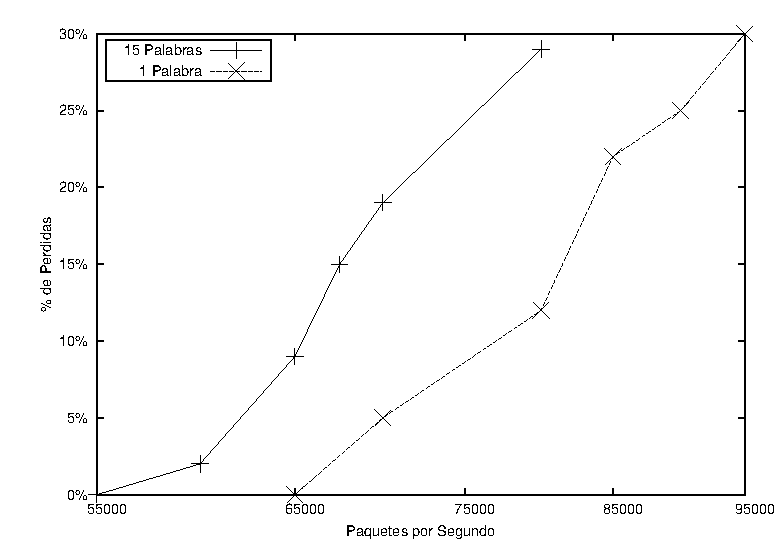
\includegraphics[width=0.7\textwidth]{5-resultados/graf/utlmax.eps}
  \caption{Retardo máximo UTL}
  \label{fig}
\end{figure}

\newpage
\subsubsection{Comparativa Inter-Algoritmos}
Se presenta a modo de comparación un gráfico que contiene el mínimo, el máximo y el promedio para el caso de una palabra con los dos algoritmos implementados. 
\begin{figure}[!h]
  \centering
	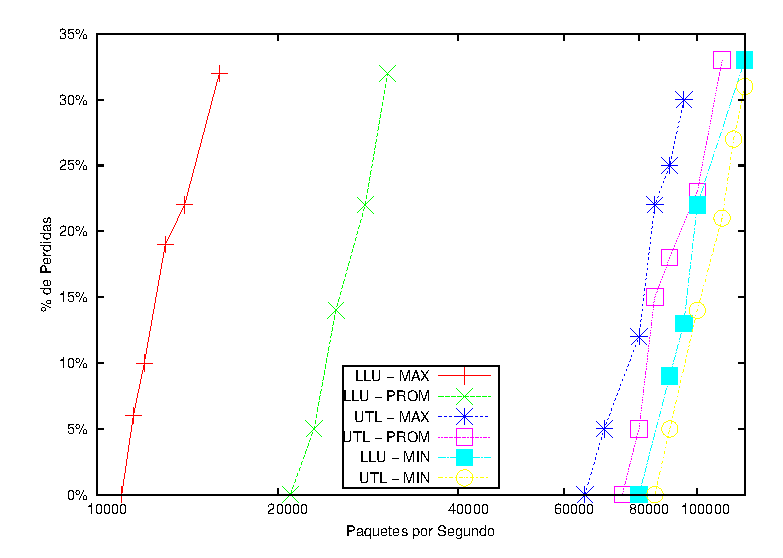
\includegraphics[width=0.7\textwidth]{5-resultados/graf/lluvsutl.eps}
  \caption{Comparativa UTL - LLU}
  \label{figvs}
\end{figure}


\newpage
\section{Cache}

La cache desarrollada para este proyecto está pensada a los fines de satisfacer la posibilidad de que varios paquetes consecutivos tengan una direcciones IP destino que pertenezcan a un grupo comun de flujos. Con la implementación utilizada se logró un tiempo de acceso uniforme de alrededor de 1000 ciclos, tiempo varias veces menor que el mejor caso tanto en LLU (6400) como en UTL (5000). En el gráfico ~\ref{fig:cachecomp} se puede ver como el peor caso del algoritmo LLU soporta hasta 10000 paquetes por segundo sin cache y hasta 700000 paquetes por segundo con la cache. Aunque este ejemplo sólo analiza el caso en el que son todos hits, es posible ver la mejora sustancial que implica una cache. 

\begin{figure}[!h]
  \centering
	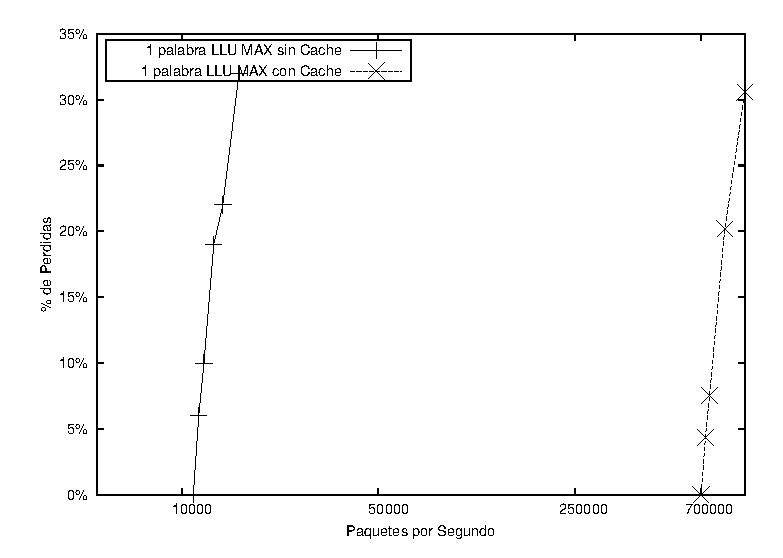
\includegraphics[width=0.7\textwidth]{5-resultados/graf/cachecomp.eps}
  \caption{Cache }
  \label{fig:cachecomp}
\end{figure}

 
\chapter{Conclusiones}


Se puede concluir que es factible implementar una arquitectura de clasificacion de paquetes en logica reprogramable combinando las velocidad del procesamiento de paquetes por Hardware con la escalabilidad y estabilidad que permite el Software. 

Consideramos que la complejidad de este tipo de proyecto reside en la implemetacion del SoC y, mas especificamente, en la curva de aprendizaje pronunciada que presentan las herramientas utilizadas para desarrollar este tipo de Sistemas. En un futuro se espera que las herramientas maduren para asi permitir una mayor fluidez y simplicidad en el diseño y puesta en marcha de este tipo de componentes. 

Por otro lado, la integración de modulos propios a un BUS pre-determinado depende fuertemente de la calidad de la documentacion que este BUS presenta, es por ello que a la hora de seleccionar un Microprocesador para integrar un SoC en logica reprogramable es fundamental revisar la documentacion y saber que se cuenta ademas con una comunidad activa y colaborativa que puedo asistir a los diseñadores durante el proceso de implementacion. 

El conjunto de conocimientos necesarios para realizar la implementacion comprende el desarrollo de Hardware, desarollo de Software y conocimiento de Redes, precisamente los tres ejes de Ingenieria en Computacion, la carrera para la cual se desarrollo este Proyecto integrador. 

Aunque se trata de una implementación experimental, la performance del sistema no se encuentra alejada de la que alcanzan los productos que se encuentran presentes en el mercado actual, y combinado con otros desarrollos realizados en el Laboratorio de Comunicaciones Digitales es posible alcanzar un producto acabado y con capacidades de resolver situaciones de la realidad.

Se destaca la Arquitectura modular implementada que, junto con el desarrollo en C++ del software, permite portar la misma a otras plataformas.

Tambien es bueno señalar que se presento una version reducida de este proyecto en CRUNIC2011.

Por ultimo, los Autores de este proyecto entienden que durante la realizacion del mismo pudieron aplicar los conceptos aprendidos durante la Carerra de Ingenieria en Computacion y desarrollar nuevas competencias. 



\subsubsection{Trabajos Futuros}

Es posible realizar varias mejoras y extensiones a este proyecto, a continuación se muestra una lista de estas mejoras futuras:

\begin{itemize}
	\item asdsad
\end{itemize}






%\section{Distribucion Lineal}
 
\backmatter
\begin{thebibliography}{10}
\bibitem{Varghese} George Varghese. \textit{Network Algorhitmics: An interdisciplinary approach to designing fast networed devices}. Morgan Kaufmann Publishers. 2005 

\bibitem{CLassif}Yaxuan Qi, Jeffrey Fong, Weirong Jiang, Bo Xu, Jun Li, Viktor Prasanna. \textit{Multi-dimensional Packet Classification on FPGA: 100 Gbps and Beyond}.

\bibitem{jumbo} Greg Ferro. \textit{Ethernet Jumbo Frames, Full Duplex and Why Jumbo Frames Are 9000 Bytes}. 2011

\bibitem{terabit}Amit Singhal, Raj Jain. \textit{Terabit switching: a survey of techniques and current products}. Computer Communications, vol 25, pp 547-556. 2002.


\bibitem{Monta} Rogelio Montañana. \textit{El nivel de red en Internet}. 2011

\bibitem{niossw} Altera Corporation. \textit{NIOS II Software Developer's Handbook}. 2011.

\bibitem{nioshw} Altera Corporation. \textit{NIOS II Hardware Development Tutorial}. 2011.

\bibitem{sopc} Altera Corporation. \textit{SOPC Builder. User Guide}. 2011.

\bibitem{avalon} Altera Corporation. \textit{Avalon Interface Specifications}. 2011.

\bibitem{avalon} Santiago Paz, Jorge Finocchietto, Carlos Zerbini. \textit{Diseño de Arquitectura Hardware Reconfigurable para la Conmutación de Paquetes en Redes Virtuales Privadas}. 2011.


\end{thebibliography}.
%\section{Distribucion Lineal}

\chapter{Apéndice A}

\section*{Configuración del Hardware}

\begin{center}
	\begin{longtable}{|l|p{4.75in}|} \hline
		\textbf{Feature} & \textbf{Description} \\ \hline
		FPGA & \begin{itemize}
			\item Cyclone II EP2C35F672C6 with EPCS16 16-Mbit serial configuration device.
			\end{itemize} \\ \hline
		I/O Interfaces &     \begin{itemize}
					\item Built-in USB-Blaster for FPGA configuration
    					\item Line In/Out, Microphone In (24-bit Audio CODEC)
   					\item Video Out (VGA 10-bit DAC)
   					\item Video In (NTSC/PAL/Multi-format)
   					\item RS232
    					\item Infrared port
   					\item PS/2 mouse or keyboard port
    					\item 10/100 Ethernet
   					\item USB 2.0 (type A and type B)
    					\item Expansion headers (two 40-pin headers)
				     \end{itemize} \\ \hline
		Memory & \begin{itemize}
					\item 8 MB SDRAM, 512 KB SRAM, 4 MB Flash
    					\item SD memory card slot
    			 \end{itemize} \\ \hline
		Displays & \begin{itemize}
					\item Eight 7-segment displays
    					\item 16 x 2 LCD display
    			 \end{itemize} \\ \hline
		Switches and LEDs & \begin{itemize}
					\item 18 toggle switches
    					\item 18 red LEDs
   					\item 9 green LEDs
   		 			\item Four debounced pushbutton switches
   				     \end{itemize} \\ \hline
		Clocks & \begin{itemize}
					\item 50 MHz clock
    					\item 27 MHz clock
   					\item External SMA clock input
   			 \end{itemize}	 \\ \hline
	\end{longtable} 
\end{center}

La FPGA incluida en la placa es una Cyclone II EP2C35 cuyas especificaciones son:

\begin{center}
	\begin{longtable}{|l|p{1.75in}|} \hline
		\textbf{Feature} & \textbf{Description} \\ \hline
		LEs & 33216 \\ \hline
		Total RAM bits & 483840 \\ \hline
		Embedded multipliers & 35 \\ \hline
		PLLs & 4 \\ \hline
		Maximum user I/O pins & 475 \\ \hline
	\end{longtable}
\end{center}

\chapter{Apéndice B}

\section*{Bus Avalon}

Avalon es una familia de interfaces para flujo de datos de alta velocidad, lectura/escritura de registros y memoria, y control de dispositivos  ``off-chip''. Existen varios tipos de bus Avalon, cuyo uso depende de las necesidades del diseño a implementar:
\begin{itemize}
	\item Avalon ST: Soporta flujo unidireccional de datos, incluyendo flujos multiplexados y paquetes.
	\item Avalon MM: Interfaz de lectura/escritura basada en memoria, típica de conexiones maestro-esclavo.
	\item Avalon Conduit Interface: Para señales que no se amoldan a los tipos anteriores.
	\item Avalon TC: Para dispositivos ``off-chip''.
	\item Avalon Interrupt Interface: Permite el envío de interrupciones entre componentes.
	\item Avalon Clock Interface: Recibe y/o distribuye señales de clock.
	\item Avalon Reset Interface.
\end{itemize}

En el diseño correspondiente a este trabajo se optó por utilizar las siguientes interfaces:

\begin{itemize}
	\item Avalon MM, debido a que los componentes están mapeados en la memoria del sistema.
	\item Avalon Clock Interface, para proveer señal de reloj al sistema.
	\item Avalon Interrupt Interface, para el componente que requiere interrumpir al procesador.
\end{itemize}

\subsubsection{Avalon MM}
Las señales de dicha interfaz necesarias para este diseño son:

\begin{itemize}
	\item address: Direcciona los datos enviados hacia y recibidos desde el procesador.
	\item chipselect: Se usa en combinacion con read/write.
	\item read: Indica una transferencia de lectura.
	\item readdata: Los datos transferidos desde el periférico hacia el procesador.
	\item write: Indica una transferencia de escritura.
	\item writedata: Los datos trasferidos desde el procesador hacia el periférico. Debe tener el mismo ancho que readdata.

\end{itemize}

\subsubsection{Avalon CLock Interface}
En este caso, la señal necesaria es
\begin{itemize}
	\item clk: Provee clock para sincronización en lógica interna y otras interfaces.
\end{itemize}

\subsubsection{Avalon Interrupt Interface}
Para esta interfaz, la señal a utilizar es

\begin{itemize}
	\item irq: Permite al periférico enviar una señal de interrupción al procesador.
\end{itemize}

\chapter{Apéndice C}

\section*{Software}

\subsection*{NIOS II SBT}

El NIOS II Software Building Tools (o SBT) es un conjunto de utilidades y scripts que sirve para crear y construir aplicaciones embebidas basadas en C/C++, librerías de usuario y paquetes de soporte de placa (board support packages o BSP). Puede invocarse desde la IDE Eclipse o desde el intérprete de comandos del NIOS II. El NIOS II SBT puede crear los siguientes tipos de proyecto:
\begin{itemize}
	\item Aplicación NIOS II: un programa que implementa alguna función deseada.
	\item NIOS II BSP: una librería que provee acceso al hardware en el sistema. Brinda un entorno de rutinas a medida para un procesador y, eventualmente, un sistema operativo. 
	\item Librería de usuario: un conjunto de funciones reutilizables. 
\end{itemize}

\subsubsection*{Aplicaciones y librerías de usuario}

Para el caso de aplicaciones y librerías de usuario, el SBT genera un makefile privado (denominado \textbf{Makefile}) el cual es usado para construir el proyecto. Al hacer esto se genera un archivo .elf para una aplicación, o .a para una librería. En este último caso, también se produce un makefile público (denominado \textbf{public.mk}), que se incluye en el privado para cualquier aplicación que use la librería de usuario.

Cuando se crea un makefile se provee al SBT con una lista de archivos de código fuente y una referencia al directorio donde se almacena el BSP. Luego, la herramienta examina la extensión de cada archivo fuente para determinar el lenguaje de programación. 

Actualmente los soportados son:

\begin{itemize}
	\item C (extensión .c).
	\item C++ (extensiones .cpp, .cxx, .cc).
	\item NIOS II Assembler (extensiones .s, .S).
\end{itemize}


\subsubsection{Board Support Packages}

Un BSP es una librería especializada que contiene código de soporte específico del sistema. La misma aisla la aplicación de los detalles del sistema, tales como mapeo de memoria, dispositivos disponibles y configuración del procesador.

Se compone de:

\begin{itemize}
	\item Capa de abstracción de hardware (Hardware Abstraction Layer o HAL): Permite al software interactuar con el hardware del sistema. Se describirá en detalle más adelante en este capítulo.
	\item Librería C estándar newlib: ANSI C estándar diseñada para sistemas embebidos.
	\item Drivers de dispositivos: para manejar cada uno de los componentes del sistema.
	\item Paquetes de software opcionales: permiten proveer funcionalidad adicional.
	\item Sistema operativo de tiempo real opcional: implementación de MicroC/OS-II RTOS.
\end{itemize}

\subsubsection*{Proceso de construcción del software}

Para crear un proyecto de software se llevan a cabo una serie de pasos:

\begin{enumerate}
	\item Se obtiene el diseño de hardware sobre el cual va a correr el software. Dicha información está almacenada en un archivo de extensión \textbf{.sopcinfo}, el cual es generado por la herramienta SOPC builder.
	\item Se genera el BSP con las características necesarias según las funcionalidades requeridas. También se genera un makefile para dicho paquete.
	\item Opcionalmente, se crea una librería de usuario (junto a su correspondiente makefile).
	\item Se escribe el software de aplicación. Se colecta todo el código fuente, y luego se genera el makefile correspondiente.
	\item Se construye el proyecto.
\end{enumerate}


\subsection *{HAL}

La capa de abstracción de hardware \textit{(Hardware Abstraction Layer o HAL)} provee una interfaz simple de drivers de dispositivos para conectar los programas con el hardware subyacente. La API está integrada con la librería estándar ANSI C, lo cual permite al software acceder a los dispositivos mediante el uso de funciones C ampliamente conocidas, tales como printf(), fopen(), fwrite(), etc.

\subsubsection*{Servicios}

La HAL provee los siguientes servicios:

\begin{itemize}
	\item Integración con la librería estándar newlib: provee funciones estándar ANSI C de amplio uso.
	\item Drivers de dispositivo: brinda acceso a cada dispositivo en el sistema.
	\item API: proporciona una interfaz estándar consistente a los servicios de la HAL, tales como acceso a dispositivos y manejo de interrupciones.
	\item Inicialización de sistema: Lleva a cabo la inicialización para el procesador y las rutinas antes de ejecutar la función principal (main).
	\item Inicialización de dispositivos: Instancia e inicializa cada uno de los dispositivos del sistema antes de que se ejecute la función main.
\end{itemize}

La figura ~\ref{fig:hal} muestra las capas de un sistema basado en la HAL, desde el nivel de hardware hasta el programa de usuario.

\begin{figure}[H]
  \centering
	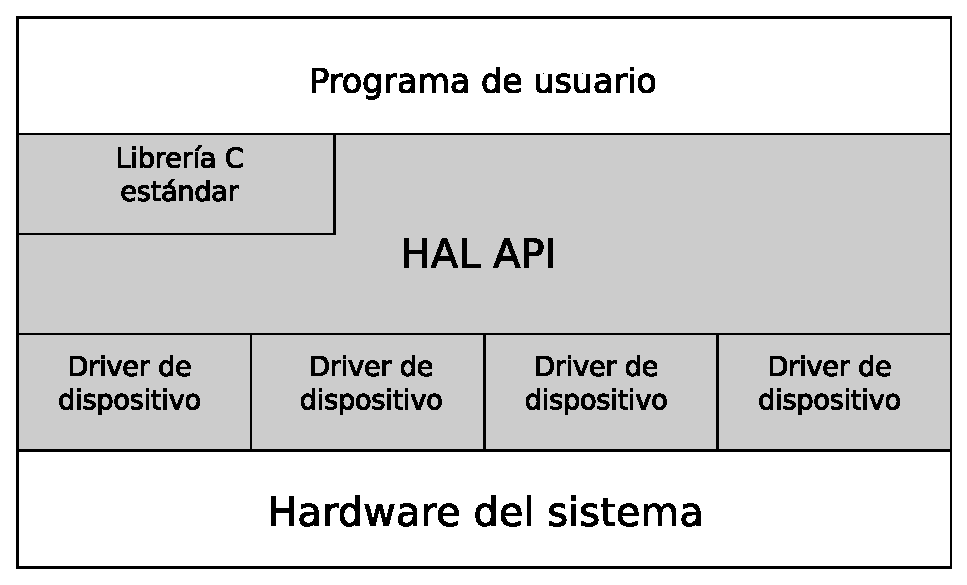
\includegraphics[width=0.80\textwidth]{3-arquitectura/graf/hal.eps}
  \caption{Capas de un sistema basado en la HAL.}
  \label{fig:hal}
\end{figure}

\subsubsection*{Modelos de dispositivos genéricos}

La HAL provee modelos de dispositivos genéricos para diversos tipos de periféricos que se encuentran en sistemas embebidos, tales como timers, interfaces Ethernet y dispositivos de I/O que transmiten datos de caracter. Estos modelos permiten escribir programas usando una API consistente sin preocuparse por el hardware subyacente. Los tipos de periféricos cubiertos son:

\begin{itemize}
	\item Dispositivos de caracter: envían y/o reciben caracteres en forma serial, como ser una UART.
	\item Timers: dispositivos que llevan la cuenta de los tics de un clock y pueden generar interrupciones periódicas.
	\item Subsistemas de archivos: un mecanismo para acceder a archivos almacenados en dispositivos físicos. Dependiendo de la implementación interna, el driver del subsistema de archivos podría acceder a los dispositivos subyacentes en forma directa o usar un driver aparte.
	\item Dispositivos Ethernet: proveen acceso a una conexión Ethernet para un stack de red, tal como la NicheStack® TCP/IP Stack, provista por Altera.
	\item Dispositivos DMA: periféricos que llevan a cabo una gran cantidad de transacciones de datos. El origen y destino pueden ser la propia memoria o algún otro dispositivo.
	\item Dispositivos con memoria flash: periféricos con memoria no volátil que utilizan un protocolo especial de programación para almacenar datos.
\end{itemize}

Todos los periféricos, ya sean de Altera o de terceros, deben proveer un archivo de cabecera que defina la interfaz de bajo nivel del dispositivo con el hardware. 

Ciertos dispositivos tienen características específicas de hardware con requerimientos de uso que no se adaptan bien a una API de propósito general. La HAL maneja dichos requerimientos mediante la función ioctl(), cuyas opciones dependerán del periférico en cuestión.

Algunos periféricos proveen funciones de acceso dedicadas que no están basadas en el modelo genérico de la HAL. En ese caso, se debe proveer un archivo de cabecera con dichas funciones.


\subsubsection*{Librería C estándar : newlib}
La HAL integra su entorno de rutinas con una implementación open-source de la librería C estándar:\textbf{ newlib}. La misma está hecha para ser utilizada en sistemas embebidos. 

\subsubsection*{La HAL dentro de un proyecto de software}
La creación y administración de proyectos basados en la HAL están altamente ligadas al NIOS II SBT. La figura ~\ref{fig:halsof} muestra el diagrama en bloques de un software basado en la HAL. Todo programa de este tipo consta de dos proyectos. El código de aplicación específico se encuentra en uno de ellos, el cual depende a su vez de otro proyecto BSP separado. El primero contiene todo el código que el programador desarrolla. El segundo, toda la información necesaria para la interacción hardware-software. Este último a su vez depende del hardware del sistema, cuya información se encuentra en un archivo generado por la herramienta SOPC Builder.

\begin{figure}[h]
  \centering
	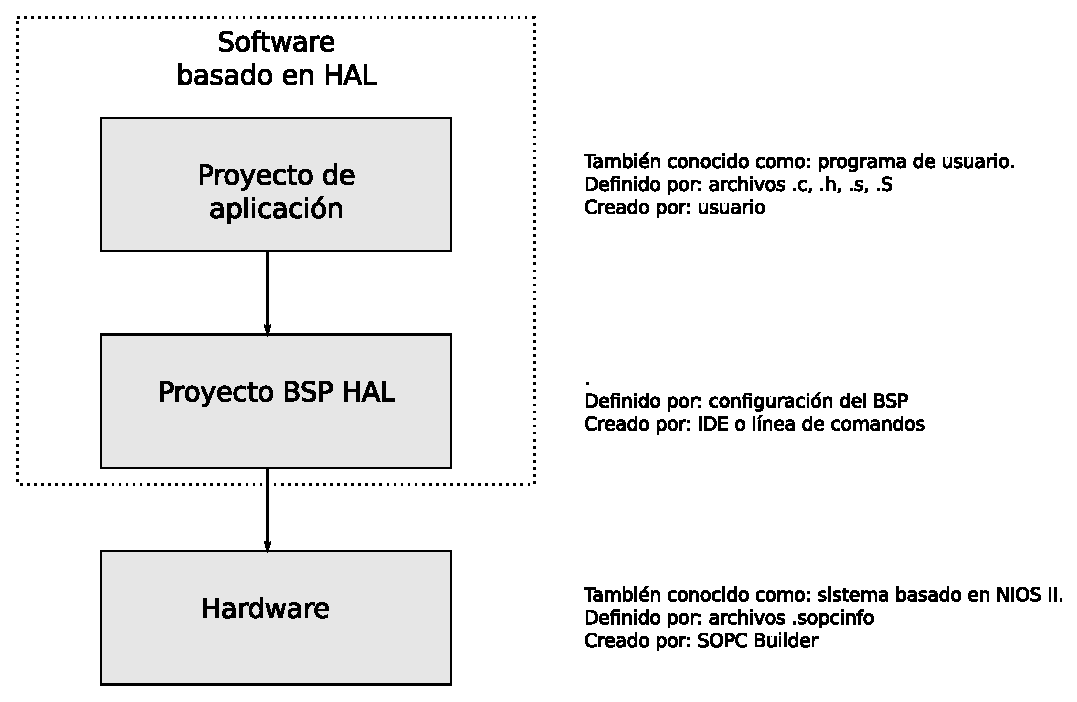
\includegraphics[width=0.90\textwidth]{3-arquitectura/graf/halsof.eps}
  \caption{Capas de un programa basado en HAL}
  \label{fig:halsof}
\end{figure}



\subsubsection*{Archivo de descripción del sistema (system.h)}
El archivo system.h provee una descripción completa del software del sistema basado en NIOS II. Describe cada periférico e incluye:

\begin{itemize}
	\item La configuración de hardware del periférico.
	\item La dirección base.
	\item Información IRQ (si es necesario).
	\item Un nombre simbólico para el periférico.
\end{itemize}

El SBT genera un archivo \textbf{system.h} para cada proyecto BSP, cuyo contenido dependerá del archivo .sopcinfo mencionado anteriormente en este capítulo.

\subsubsection*{Acceso al hardware}
El software accede al hardware a través de macros que abstraen la interfaz mapeada en memoria al dispositivo. Todos los componentes proveen un directorio que define el hardware y el software del periférico en cuestión. En esta carpeta se encuentra un archivo de cabecera que define la interfaz con el hardware y su nombre es $<componente>$\_regs.h, el cual se incluye en el subdirectorio inc. Por ejemplo, el componente JTAG UART define su interfaz en el archivo $<Directorio Instalacion Altera>$/ip/altera/sopc\_builder\_ip/

altera\_avalon\_jtag\_uart/inc/altera\_avalon\_jtag\_uart\_regs.h.

El archivo de cabecera \_regs.h define las siguientes macros de acceso para el componente:
\begin{itemize}
	\item Macros de acceso a registros que proveen operaciones de lectura/escritura. Éstas son:
	\begin{itemize}
		\item IORD\_$<NombreDelComponente>$\_$<NombreDelRegistro>$ ($<DireccionBaseDelComponente>$).
		\item IOWR\_$<NombreDelComponente>$\_$<NombreDelRegistro>$ ($<DireccionBaseDelComponente>$, $<Dato>$).
	\end{itemize}
	\item Macros de direccionamiento de registro, que retornan las direcciones físicas de cada uno de ellos. La dirección devuelta es la dirección base del componente + el valor de desplazamiento de registro especificado. Esta macro tiene el nombre de esta forma:
	\begin{itemize}
		\item IOADDR\_$<NombreDelComponente>$\_$<NombreDelRegistro>$ ($<DireccionBaseDelComponente>$).
	\end{itemize}
	\item Máscaras a nivel de bits. Estas macros tienen los siguientes nombres:
	\begin{itemize}
		\item $<NombreDelComponente>$\_$<NombreDelRegistro>$\_$<NombreDelCampo>$\_MSK : Máscara de bit de un campo.
		\item $<NombreDelComponente>$\_$<NombreDelRegistro>$\_$<NombreDelCampo>$\_OFST : Desplazamiento de bit del el comienzo del campo.
	\end{itemize}
\end{itemize}

Cabe mencionar que las los valores leídos/escritos mediante las macros de acceso a registro (IORD e IOWR) no trabajan con la caché del microprocesador.
En este contexto, es necesario destacar esto ya que los valores intercambiados entre el módulo software y el gestor de datos tienen que ser leidos/escritos solamente si estos están en el bus.

\chapter{Apéndice D}
\section*{SOPC Builder}

SOPC Builder es una herramienta que posibilita la definición y generación de Sistemas en Chips Programables (system-on-a-programable-chip, SOPC) en mucho menos tiempo que requieren los métodos manuales tradicionales de integración. Es parte del software Quartus II.

\subsection*{Componentes a medida (Custom Component)}

Además de una lista de componentes que ya están preparados para funcionar, SOPC Builder ofrece la posibilidad de crear componentes personalizados. Esto se efectúa importando módulos creados en algún HDL.

 Para integrarlos al diseño del sistema se siguen los siguientes pasos:
\begin{enumerate}
	\item Determinar las interfaces necesarias para interactuar con el componente.
	\item Crear la lógica del componente con algún HDL.
	\item Usar el editor de componentes de SOPC Builder para crear el componente a partir de los archivos HDL.
	\item Instanciar el componente en el sistema 
\end{enumerate}

\begin{figure}[H]
  \centering
	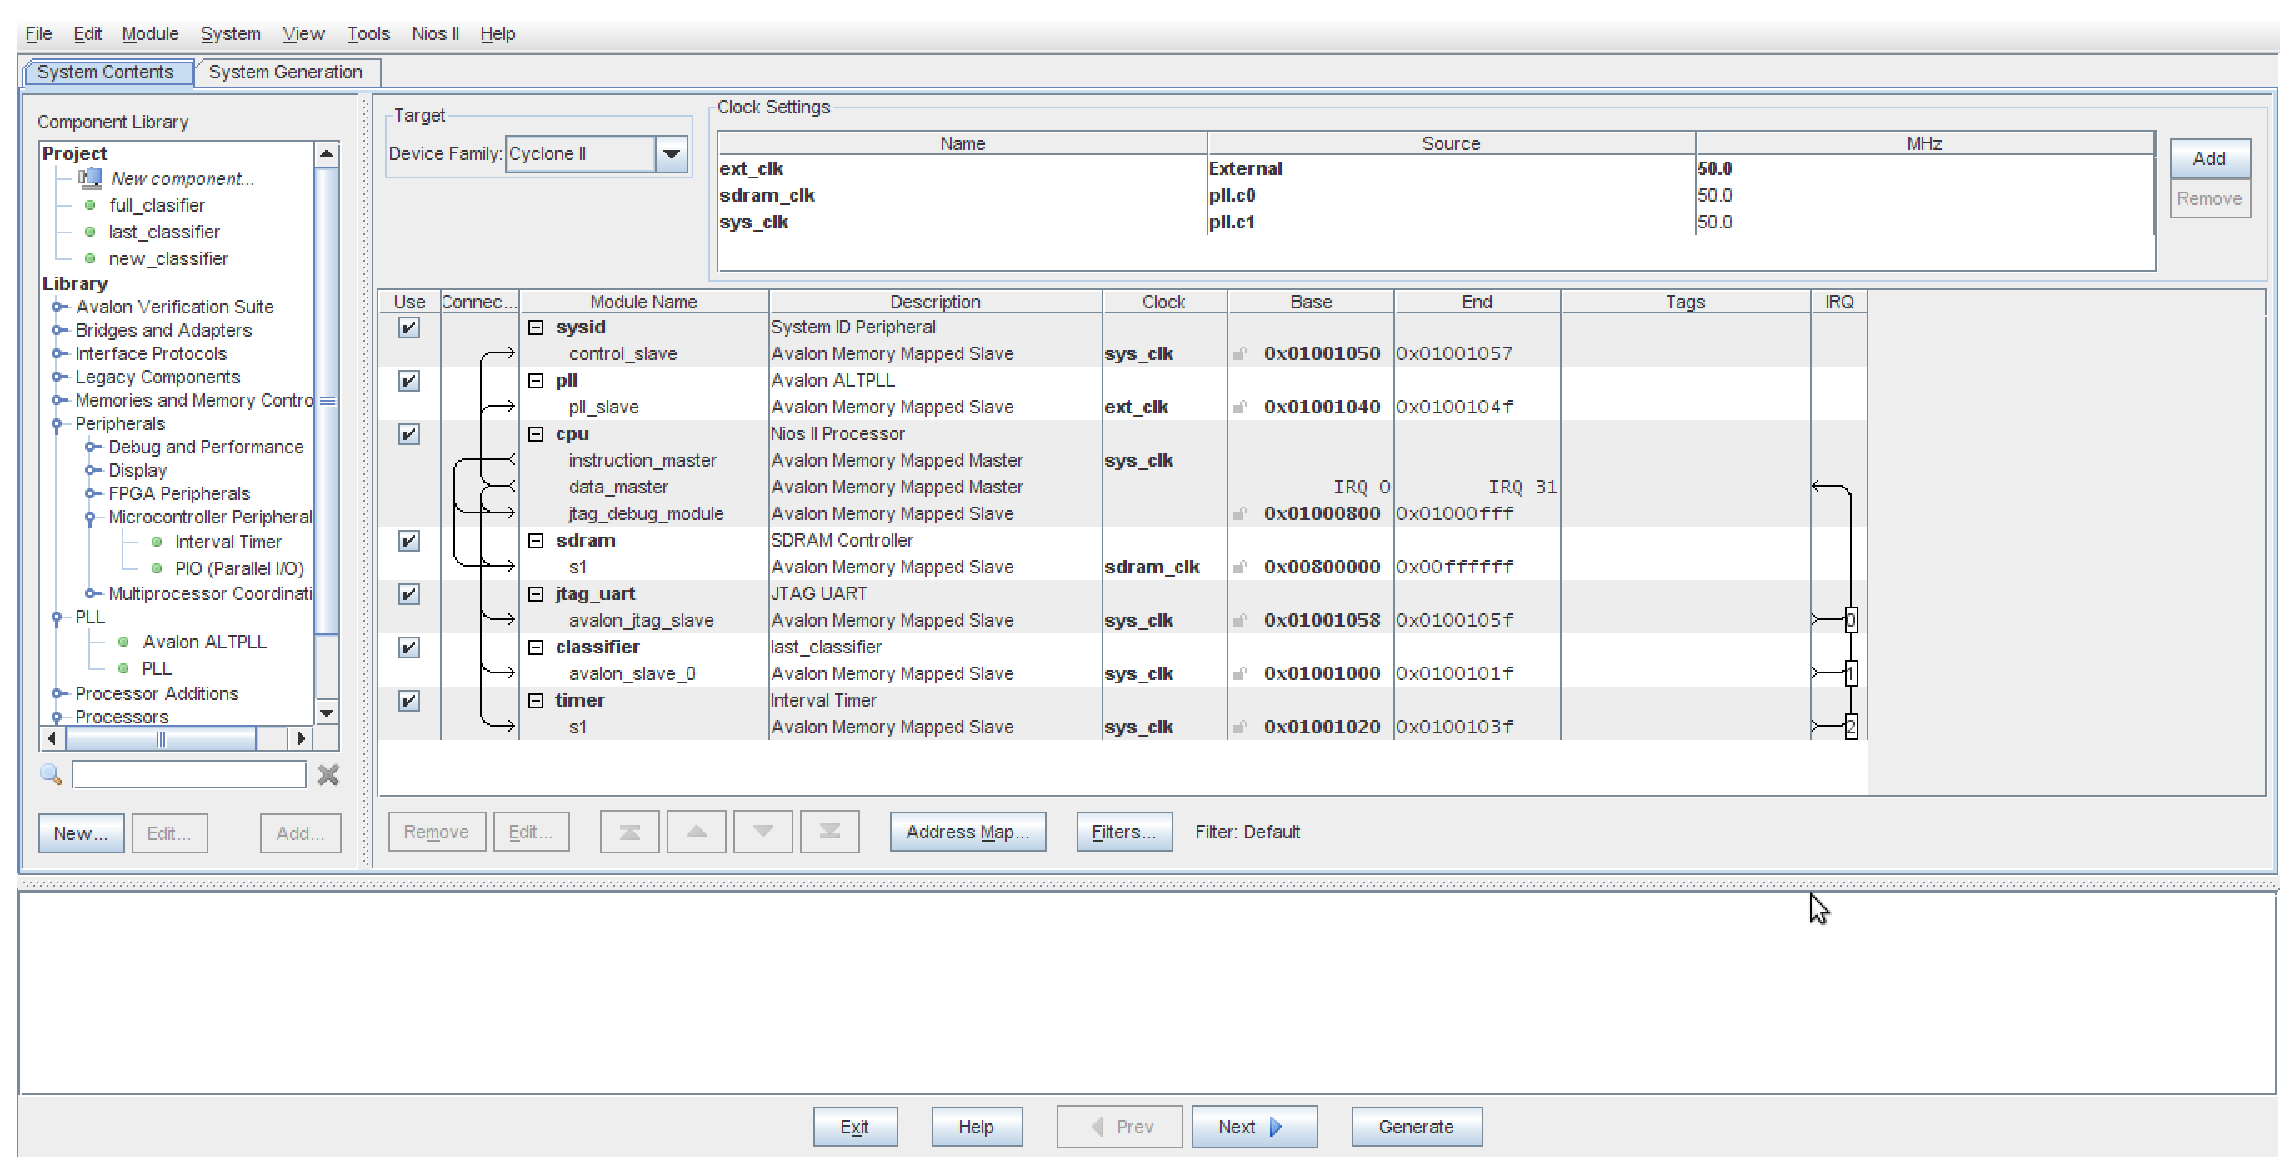
\includegraphics[width=0.90\textwidth]{8-apendices/graf/sopc1.eps}
  \caption{Ventana principal del SOPC Builder}
  \label{fig:sopc1}
\end{figure}

\begin{figure}[H]
  \centering
	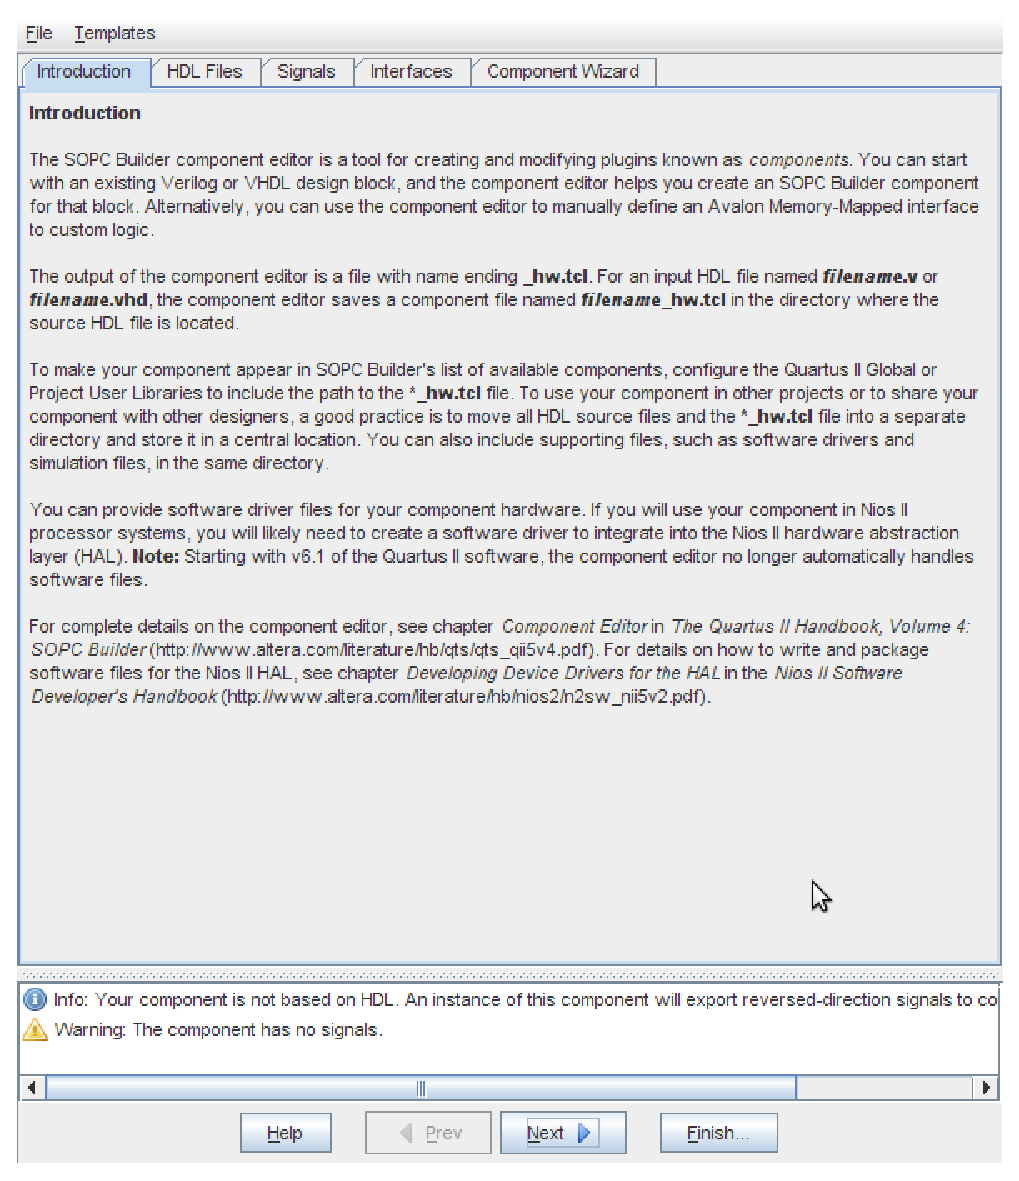
\includegraphics[width=0.60\textwidth]{8-apendices/graf/sopc2.eps}
  \caption{Generador de componentes}
  \label{fig:sopc2}
\end{figure}


\end{document}              % fin del documento
